\documentclass[12pt, a4paper]{report}
\usepackage{hyperref}
\usepackage[top=3cm,right=3cm,bottom=3cm,left=2.5cm]{geometry}
\usepackage{caption}
\usepackage{indentfirst}
\usepackage{graphicx}
\usepackage{subfigure}
\usepackage{float}
\usepackage{amsmath}
\usepackage{listings} % Load the listings package
\usepackage{xcolor}   % Optional: For custom colors
\usepackage{tikz}
\usetikzlibrary{shapes.geometric, arrows.meta} % Use arrows.meta library
\usepackage{fancyhdr}
\usepackage{pdfpages}

\usepackage{hyperref}


\usepackage{xepersian}
\settextfont{XB Zar}
\linespread{1.2}
\setcounter{secnumdepth}{2}
\setcounter{tocdepth}{2}



\pagestyle{fancy}
% Set up fancyhdr to place page number at the top left
\pagestyle{fancy}
\fancyhf{} % Clear all header/footer fields
\fancyhead[L]{\thepage} % Page number on the top left

% Define custom style for chapter page (no header or footer)
\fancypagestyle{plain}{
	\fancyhf{} % Clear headers and footers
	\renewcommand{\headrulewidth}{0pt} % Remove header rule
}


% Changing TOC addressing format (from period separation to dash seperation)
\renewcommand{\thesection}{\thechapter-\arabic{section}-}
\renewcommand{\thesubsection}{\thechapter-\arabic{section}-\arabic{subsection}-}
\renewcommand{\thesubsubsection}{\thechapter-\arabic{section}-\arabic{subsection}-\arabic{subsubsection}-}

\renewcommand{\thetable}{(\thechapter-\arabic{table})}

% Redefine how captions are written 
\renewcommand{\thefigure}{(\thechapter-\arabic{figure})}

% Set caption font size to 11pt
\captionsetup{font=small, labelsep=space} % 'small' is equivalent to 11pt in most classes

% Make sure Persian and Latin text have their respective font sizes
\settextfont{XB Zar} % Persian font
\setlatintextfont{Times New Roman} % Latin font

% Automatically switch between Persian and Latin fonts based on character type
\XeTeXinterchartokenstate=1
\newXeTeXintercharclass\persianchars
\newXeTeXintercharclass\latinchars

% Automatically switch fonts when switching between Persian and Latin characters
\XeTeXinterchartoks \latinchars \persianchars = {\begingroup\persianfont\endgroup}
\XeTeXinterchartoks \persianchars \latinchars = {\begingroup\latinfont\endgroup}


\setlatintextfont{Courier New} % برای نمایش کدهای انگلیسی
\lstset{
	language=C++,                      % Set language to C++
	basicstyle=\ttfamily\small,        % Use monospaced font
	keywordstyle=\bfseries\color{blue}, % Keywords in bold blue
	stringstyle=\color{red},           % Strings in red
	commentstyle=\itshape\color{green!60!black}, % Comments in green italics
	numbers=right,                     % Line numbers on the right
	numberstyle=\tiny,                 % Line number font size
	stepnumber=1,                      % Show line numbers every line
	frame=single,                      % Add a frame around code
	tabsize=4,                         % Set tab size
	showstringspaces=false,            % Do not show spaces in strings
	xleftmargin=10pt,                  % Adjust left margin for better alignment
	xrightmargin=10pt                  % Adjust right margin for better alignment
}





\title{گزارش کارآموزی}
\author{عسل خائف}

\begin{document}
	%\maketitle
	\begin{titlepage}
		\centering
		% University logo
		
\includegraphics[width=0.4\textwidth]{img/university-logo.png}
		
		% University and Faculty name
		{\Large دانشگاه اصفهان}\par
		{\Large دانشکده مهندسی کامپیوتر}\par\vspace{2cm}
		
		% Report title
		\textbf
		{\Huge گزارش پروژه زبان‌های برنامه نویسی}\par\vspace{1.5cm}
		{\Huge زبان برنامه نویسی \lr{C++}}\par\vspace{1.5cm}
		
		% Intern details
		\large
		\textbf{تهیه کنندگان:}\par{متین اعظمی}\par{پوریا طلائی}\par{عسل خائف}\par\vspace{1cm}  

		\textbf{استاد درس:}\par{آقای دکتر آرش شفیعی}\par\vspace{3cm}
		
		\par{نیم‌سال اول ۴۰۳ - ۴۰۴}\par\vspace{0.5cm}
				
		
	\end{titlepage}
	\tableofcontents
	\listoftables
	
	
\chapter{مقدمه}
\section{تاریخچه زبان C++}
\begin{itemize}
	\item
آغاز و ابداع زبان \lr{C++}: 
زبان \lr{C++} توسط بیارنه استراستروپ  (\lr{Bjarne Stroustrup}) در اوایل دهه 1980 در \lr{Bell Labs} شرکت\lr{ (AT-T)} توسعه داده شد.
 این زبان در ابتدا به‌عنوان یک نسخه ارتقاء یافته از زبان \lr{C}  طراحی شد که ویژگی‌های شی‌گرا به آن افزوده می‌شد.
 به‌ویژه هدف آن این بود که برنامه‌نویسان قادر به نوشتن برنامه‌های پیچیده‌تر با ویژگی‌های شی‌گرا باشند، در حالی که هنوز از کارایی بالا و قابلیت‌های زبان \lr{C} بهره‌مند باشند.
	
	\item
هدف اولیه: \lr{C++}  ابتدا به‌منظور ایجاد یک زبان برنامه‌نویسی با پشتیبانی از برنامه‌نویسی شی‌گرا (\lr{OOP}) در کنار قابلیت‌های سطح پایین زبان \lr{C} طراحی شد. ویژگی‌های \lr{OOP} مانند ارث‌بری (\lr{inheritance})، چندریختی (\lr{polymorphism})  و کپسوله‌سازی (\lr{encapsulation}) به این زبان اضافه شدند تا برنامه‌نویسان قادر باشند کدهای پیچیده‌تر و قابل نگهداری‌تری بنویسند.
	
	\item
نام‌گذاری \lr{C++}: نام \lr{C++} به دلیل افزوده شدن ویژگی‌های جدید به زبان \lr{C} انتخاب شد. علامت ++ به‌طور نمادین به افزایش یا ارتقای زبان \lr{C} اشاره دارد.
	
\end{itemize}

\section{کاربردهای زبان C++}
\begin{itemize}
		\item
سیستم‌های نرم‌افزاری پیچیده: \lr{C++} از ابتدا برای نوشتن سیستم‌های پیچیده و نرم‌افزارهای کاربردی طراحی شد که نیاز به سرعت بالا و دسترسی مستقیم به سخت‌افزار دارند. از این رو در سیستم‌عامل‌ها مانند (ویندوز و لینوکس) ، نرم‌افزارهای سیستمی و نرم‌افزارهای \lr{Embedded} به‌طور گسترده‌ای استفاده می‌شود.
	\item
توسعه بازی‌ها: \lr{C++} زبان اصلی برای توسعه بازی‌های کامپیوتری و گرافیکی است. موتورهای بازی‌سازی بزرگی مانند \lr{Unreal Engine }از C++ استفاده می‌کنند. این زبان به دلیل کارایی بالا و پشتیبانی از برنامه‌نویسی شی‌گرا برای توسعه بازی‌های پیچیده بسیار مناسب است.
	\item
برنامه‌نویسی علمی و مهندسی: \lr{C++} در زمینه‌هایی مانند شبیه‌سازی‌های علمی، پردازش تصویر، پردازش داده‌های بزرگ و مدل‌سازی فیزیکی استفاده می‌شود. به‌ویژه در حوزه‌های مهندسی و علوم کامپیوتر به دلیل قدرت پردازشی بالا و مدیریت دقیق حافظه کاربرد زیادی دارد.
	\item
نرم‌افزارهای مالی: به دلیل سرعت و کارایی بالای \lr{C++}، این زبان در توسعه نرم‌افزارهای مالی، تحلیل داده‌های بورس و مدیریت تراکنش‌های بانکی نیز کاربرد دارد.
\end{itemize}
\section{هدف اصلی از طراحی C++}
\begin{itemize}
	\item
رفع مشکلات زبان C : \lr{C}++ به‌عنوان یک ارتقاء بر زبان \lr{C} طراحی شد. یکی از مشکلات زبان C عدم پشتیبانی از ویژگی‌های شی‌گرا بود که در برنامه‌های پیچیده کارایی و نگهداری کد را دشوار می‌کرد. \lr{C++} این قابلیت‌ها را به زبان اضافه کرد، در حالی که همچنان از ساختارهای سطح پایین و کارایی بالای \lr{C} بهره می‌برد.
\item
افزایش قدرت و انعطاف‌پذیری: \lr{C++} از همان ابتدا قصد داشت تا قدرت و انعطاف‌پذیری بیشتری را به برنامه‌نویسان بدهد. به‌ویژه با استفاده از ویژگی‌های شی‌گرا، کدهای پیچیده‌تر و انعطاف‌پذیرتری می‌توان نوشت.
\item
پشتیبانی از برنامه‌نویسی شی‌گرا: یکی از اصلی‌ترین اهداف \lr{C++} این بود که ویژگی‌های شی‌گرا را به زبان \lr{C} اضافه کند، به‌طوری که برنامه‌نویسان بتوانند از ارث‌بری، چندریختی و کپسوله‌سازی برای نوشتن نرم‌افزارهای مقیاس‌پذیرتر و قابل نگهداری‌تر استفاده کنند.
\end{itemize}
\section{ مشکلات اولیه زبان C++}
\begin{itemize}
	\item
پیچیدگی: یکی از مشکلات ابتدایی \lr{C++ } پیچیدگی یادگیری آن بود. بسیاری از برنامه‌نویسان جدید با مفاهیم پیچیده‌ای مانند اشاره‌گرها، مدیریت حافظه دستی و ویژگی‌های شی‌گرا مواجه می‌شدند.
\item 
مدیریت حافظه: اگرچه \lr{ C++} به برنامه‌نویسان کنترل دقیقی بر حافظه می‌دهد، اما این امر باعث می‌شود که مدیریت حافظه به‌صورت دستی بسیار دشوار و مستعد خطا باشد. برای مثال، دسترسی به حافظه اشتباه یا فراموش کردن آزادسازی حافظه می‌تواند باعث ایجاد اشکالاتی مانند "\lr{Memory Leaks}" و "\lr{Segmentation Faults}" شود.
\item 
عدم تطابق با زبان‌های سطح بالا: در ابتدا، بسیاری از برنامه‌نویسان سعی می‌کردند تا \lr{C++} را مانند زبان‌های سطح بالاتر استفاده کنند، اما این امر به‌خاطر پیچیدگی‌های خاص \lr{C++ }و نیاز به توجه بیشتر به جزئیات سخت‌افزاری ممکن نبود.
\end{itemize}



برای ارزیابی زبان C++ در مقایسه با زبان‌های دیگر و به‌ویژه زبان‌هایی که ویژگی‌های مشابه دارند، باید معیارهای مختلفی از جمله خوانایی، قابلیت اطمینان، کارایی، هزینه یادگیری و بهره‌وری، و قابلیت جابجایی را در نظر بگیریم. در اینجا یک تحلیل جامع از C++ در مقایسه با زبان‌های مشابه (مانند C , Java، Python) ارائه می‌شود:

\section{ویژگی‌های خاص C++ که آن را از زبان‌های مشابه متمایز می‌کند}
\begin{itemize}
\item 
کنترل دقیق بر حافظه: یکی از بزرگترین ویژگی‌های تمایز \lr{C++} نسبت به زبان‌های مشابه، قابلیت کنترل دقیق بر حافظه است. در زبان‌هایی مانند \lr{C}  و \lr{C++}، برنامه‌نویس باید به‌صورت دستی حافظه را تخصیص دهد و آن را آزاد کند. این ویژگی به زبان‌های سطح پایین‌تر این امکان را می‌دهد که از عملکرد بسیار بالا و بهینه استفاده کنند، به‌ویژه در سیستم‌های \lr{embedded} و بازی‌ها. این ویژگی در زبان‌هایی مانند \lr{Java}  و \lr{Python}  وجود ندارد، زیرا این زبان‌ها از جمع‌آوری زباله (\lr{garbage collection}) برای مدیریت حافظه استفاده می‌کنند.
\item 
شی‌گرایی و چندریختی : C++ از اولین زبان‌هایی بود که پشتیبانی از ویژگی‌های شی‌گرایی را به زبان‌های سطح پایین اضافه کرد. این ویژگی در مقایسه با زبان‌هایی مثل C  که شی‌گرایی ندارند، یک مزیت بزرگ به‌شمار می‌آید. به علاوه،  \lr{C++} از چندریختی (\lr{polymorphism}) و وراثت (\lr{inheritance}) به‌خوبی پشتیبانی می‌کند که این امر نوشتن کدهای پیچیده و قابل نگهداری را ساده‌تر می‌کند.
\item 
توانایی ترکیب ویژگی‌های سطح پایین و بالا: \lr{C++ }یک زبان چندپارادایمی است که هم از برنامه‌نویسی شی‌گرا (\lr{OOP}) و هم از ویژگی‌های سطح پایین مانند دسترسی مستقیم به حافظه، کار با پورت‌ها و سخت‌افزار پشتیبانی می‌کند. این ویژگی باعث می‌شود که \lr{C++ }برای توسعه نرم‌افزارهای سیستم و برنامه‌های پیچیده با نیاز به کارایی بالا ایده‌آل باشد.
\item 
پشتیبانی از \lr{Template} و \lr{Generic Programming}: \lr{C++} دارای قابلیت‌های پیشرفته‌ای مانند \lr{Templates} است که امکان برنامه‌نویسی جنریک را فراهم می‌کند. این ویژگی به برنامه‌نویسان این امکان را می‌دهد که کدهای بازتر و انعطاف‌پذیرتری بنویسند که برای انواع مختلف داده‌ها کار کند.
\end{itemize}

\section{ارزیابی زبان C++ بر اساس معیارهای مختلف}
\subsection{خوانایی (Readability)}
\begin{itemize}
	\item 
 \lr{:C++}   به‌طور کلی، خوانایی C++ نسبت به زبان‌های سطح بالا مانند \lr{Python}  یا  \lr{Java} پایین‌تر است. دلیل این امر استفاده از ویژگی‌های پیچیده‌ای مانند اشاره‌گرها (\lr{pointers}) ، چندپارادایم بودن زبان، و نیاز به مدیریت حافظه دستی است. این ویژگی‌ها ممکن است باعث پیچیدگی در فهم کد و اشکال‌زدایی آن شوند.
\item 
\lr{:Java/Python} این زبان‌ها به‌خاطر سادگی و ساختار واضح‌تر خود، خوانایی بیشتری دارند. در \lr{Python} به‌ویژه با وجود سینتکس ساده‌تر و نداشتن ویژگی‌هایی مانند اشاره‌گر، کدها بسیار قابل فهم‌تر هستند.
\end{itemize}
\subsection{قابلیت اطمینان (Reliability) }
\begin{itemize}
	\item
\lr{:C++} یکی از نقاط ضعف \lr{C++ }در مقایسه با زبان‌هایی مانند Java ،خطراتی مانند \lr{Memory Leaks }و \lr{Segmentation \lr{Faults} }است. زیرا \lr{C++ }به‌طور دستی حافظه را مدیریت می‌کند و این می‌تواند منجر به مشکلاتی در صورت خطای برنامه‌نویس شود. با این حال، این ویژگی برای سیستم‌های پیچیده و بازی‌ها که نیاز به کارایی بالا دارند، بسیار مفید است.
\item
\lr{Java}: \lr{Java}  با استفاده از \lr{garbage collection} و مدیریت خودکار حافظه، قابلیت اطمینان بیشتری دارد و کمتر مستعد مشکلات ناشی از مدیریت حافظه است.
\item
\lr{Python}: \lr{Python} نیز مانند \lr{Java} از \lr{garbage collection} استفاده می‌کند و به همین دلیل بیشتر از \lr{C++ }قابلیت اطمینان دارد، به‌ویژه در پروژه‌های بزرگتر که مدیریت حافظه مشکل‌ساز می‌شود.
\end{itemize}
\subsection{کارایی (Performance) }
\begin{itemize}
	\item
\lr{:C++}  \lr{C++}یکی از سریع‌ترین زبان‌های برنامه‌نویسی است. به‌خاطر آنکه برنامه‌نویسان کنترل دقیقی بر حافظه دارند، می‌توانند به بهینه‌ترین شکل ممکن از منابع استفاده کنند. این زبان برای برنامه‌هایی که به کارایی بالا نیاز دارند) مثل بازی‌ها، سیستم‌عامل‌ها و برنامه‌های(real-time  بسیار مناسب است.
\item
\lr{:Java/Python } مقابل، زبان‌های سطح بالاتر مانند \lr{Java}  و \lr{Python}  معمولاً از سرعت پایین‌تری برخوردارند، زیرا خودکار حافظه را مدیریت می‌کنند و به همین دلیل نیاز به منابع بیشتری دارند. \lr{Python} به‌ویژه به‌خاطر مفسر بودنش کندتر از \lr{C++} است.
\end{itemize}
\subsection{هزینه یادگیری و برنامه‌نویسی \lr{(Learning Curve and Development Costs) }}
\begin{itemize}
	\item
\lr{ :C++ }یادگیری \lr{C++ }می‌تواند چالش‌برانگیز باشد، به‌ویژه برای مبتدیان. مفاهیم پیچیده‌ای مانند اشاره‌گرها، مدیریت حافظه دستی، و ویژگی‌های شی‌گرایی نیازمند زمان و تلاش برای یادگیری و درک عمیق هستند. این زبان برای برنامه‌نویسان مبتدی و تازه‌کار ممکن است دشوار باشد.
\item
\lr{:Java/Python } در مقایسه،\lr{Python}‌خاطر سینتکس ساده‌اش بسیار سریع‌تر یاد گرفته می‌شود و برای برنامه‌نویسان مبتدی مناسب         است. \lr{Java} نیز اگرچه کمی پیچیده‌تر از \lr{Python} است، اما از \lr{C++} ساده‌تر است و برای یادگیری و توسعه سریع‌تر از C++ است.
\end{itemize}
\subsection{ هزینه اجرایی \lr{(Execution Cost and Efficiency)} }
\begin{itemize}
	\item
:C++ یکی از نقاط قوت C++ این است که برنامه‌های نوشته شده با آن معمولاً از کمترین منابع سخت‌افزاری استفاده می‌کنند و سریع‌ترین عملکرد را دارند.
\item
:Java/Python  در حالی که  \lr{Java} و \lr{Python}به دلیل نیاز به ماشین مجازی یا مفسر و مدیریت حافظه خودکار، از نظر کارایی نسبت به C++ کندتر عمل می‌کنند
.
\end{itemize}
\subsection{ قابلیت جابجایی  (Portability)}
\begin{itemize}
	\item
\lr{:C++}  \lr{C++}برنامه‌ها را به کد ماشین تبدیل می‌کند، به همین دلیل ممکن است برای پلتفرم‌های مختلف نیاز به کامپایل مجدد داشته باشد.
	\item
\lr{:Java }یکی از مزایای اصلی \lr{Java} این است که برنامه‌های نوشته شده با آن از ویژگی \lr{"write once, run anywhere"} برخوردار هستند.
 زیرا کد جاوا به بایت‌کد تبدیل شده و در \lr{Java Virtual Machine (JVM)}  اجرا می‌شود که این امکان را می‌دهد تا بدون تغییر کد بر روی هر پلتفرم قابل اجرا باشد.
 	\item
\lr{:Python} \lr{Python}  نیز به‌خاطر پشتیبانی از پلتفرم‌های مختلف، از جمله ویندوز، لینوکس، و مک، دارای قابلیت جابجایی خوبی است.
\end{itemize}
\subsection{نتیجه‌گیری}
\lr{C++ }از نظر کارایی و کنترل دقیق بر منابع بسیار قدرتمند است و در برنامه‌هایی که نیاز به بهینه‌سازی‌های پیچیده دارند، ایده‌آل است.
برای برنامه‌هایی که نیاز به سادگی و سرعت توسعه دارند، زبان‌هایی مانند  \lr{Python} یا \lr{Java}  ممکن است گزینه‌های بهتری باشند.
اگر به دنبال توسعه سیستم‌های پیچیده و مقیاس‌پذیر با قابلیت‌های پیشرفته مانند \lr{OOP} و کنترل دقیق هستید،\lr{ C++ }انتخاب بسیار مناسبی است.
\section{پیاده‌سازی زبان C++: کامپایلر یا مفسر؟}
\begin{itemize}
	 	\item
	زبان \lr{C++ } به‌طور کامل به کد ماشین ترجمه می‌شود، که پس از آن مستقیماً توسط سیستم‌عامل و سخت‌افزار اجرا می‌شود. به این معنی که C++  یک زبان کامپایل‌شده است، نه یک زبان مفسر.
	 	\item
	در این فرآیند، ابتدا کد منبع \lr{C++} توسط کامپایلر ترجمه می‌شود به کدهای ماشین یا بایت‌کدهایی که مستقیماً قابل اجرا روی سیستم هدف باشند. این کامپایلرها مسئول تبدیل کدهای نوشته‌شده در \lr{C++ }به فرم قابل اجرا هستند.
\end{itemize}
\section{ کامپایلرهای رایج برای زبان C++}
در حال حاضر چندین کامپایلر برای زبان C++ وجود دارد که هر یک ویژگی‌های خاص خود را دارند. برخی از محبوب‌ترین کامپایلرها عبارتند از:

\subsection{\lr{GCC (GNU Compiler Collection)}}
\textbf{توسعه‌دهنده:} \lr{GNU (Free Software Foundation).}

\textbf{مزایا:}
\begin{itemize}
	\item \textbf{منبع باز:} GCC یک کامپایلر منبع‌باز است و در بیشتر سیستم‌های عامل لینوکس و یونیکس استفاده می‌شود.
	\item \textbf{پشتیبانی از استانداردهای جدید \lr{:C++}} GCC به‌طور مداوم با ویژگی‌های جدید C++ همگام است و از اکثر استانداردهای جدید \( C++ \) از جمله \( C++11 \)، \( C++14 \)، \( C++17 \)، و \( C++20 \) پشتیبانی می‌کند.
	\item \textbf{قابلیت‌های بهینه‌سازی:} \lr{GCC} یکی از کامپایلرهای معروف برای بهینه‌سازی کد است که سرعت اجرای برنامه‌ها را بهبود می‌بخشد.
	\item \textbf{پشتیبانی از پلتفرم‌های مختلف:} \lr{GCC} قابلیت کار بر روی سیستم‌های مختلف مانند لینوکس، مک، ویندوز از طریق \lr{Cygwin} و \lr{MinGW} را دارد.
\end{itemize}

\textbf{معایب:}
\begin{itemize}
	\item در مقایسه با کامپایلرهای تجاری، ممکن است بعضی از ویژگی‌ها یا بهینه‌سازی‌ها در \lr{GCC} کمتر دقیق یا بهینه باشند.
\end{itemize}

\subsection{Clang}
\textbf{توسعه‌دهنده:} \lr{Apple Inc}. با مشارکت پروژه‌های متن‌باز.

\textbf{مزایا:}
\begin{itemize}
	\item \textbf{سرعت کامپایل بالا:} \lr{Clang} به‌عنوان یک کامپایلر سریع شناخته می‌شود که سرعت کامپایل بالاتری نسبت به برخی از دیگر کامپایلرها دارد.
	\item \textbf{پیغام‌های خطای دقیق و مفصل:} یکی از ویژگی‌های برجسته \lr{Clang} پیغام‌های خطای بسیار واضح و دقیق آن است که برای برنامه‌نویسان مبتدی و حرفه‌ای مفید است.
	\item \textbf{پشتیبانی از استانداردهای جدید:} \lr{Clang} همچنین از استانداردهای جدید C++ پشتیبانی می‌کند.
	\item \textbf{پشتیبانی از پلتفرم‌های مختلف:} مانند \lr{GCC}، \lr{Clang }نیز قابلیت اجرا بر روی پلتفرم‌های مختلف را دارد.
	\item \textbf{یکپارچگی با ابزارهای \lr{:Apple}} به‌ویژه در محیط‌های \lr{macOS} و \lr{iOS}، \lr{Clang} کامپایلر پیش‌فرض است.
\end{itemize}

\textbf{معایب:}
\begin{itemize}
	\item برخی از ویژگی‌های خاص بهینه‌سازی \lr{Clang} ممکن است نسبت به \lr{GCC} کمتر پخته باشد.
\end{itemize}

\subsection{\lr{Microsoft Visual C++ (MSVC)}}
\textbf{توسعه‌دهنده:} \lr{Microsoft}.

\textbf{مزایا:}
\begin{itemize}
	\item \textbf{یکپارچگی با ویژوال استودیو:} \lr{MSVC} به‌طور کامل با محیط توسعه‌ی \lr{Visual Studio} که یکی از محبوب‌ترین \lr{IDE} ها است، یکپارچه شده است. این یکپارچگی به برنامه‌نویسان C++ این امکان را می‌دهد که به راحتی برنامه‌های C++ را در ویندوز توسعه دهند.
	\item \textbf{ابزارهای پشتیبانی قوی:} \lr{MSVC} ابزارهای زیادی برای اشکال‌زدایی و بهینه‌سازی کدها ارائه می‌دهد که برای توسعه نرم‌افزارهای ویندوزی بسیار مفید است.
	\item \textbf{بهینه‌سازی برای ویندوز:} \lr{MSVC} برای بهینه‌سازی کدهایی که روی پلتفرم ویندوز اجرا می‌شوند، بسیار مناسب است.
\end{itemize}

\textbf{معایب:}
\begin{itemize}
	\item MSVC معمولاً در مقایسه با \lr{GCC} یا \lr{Clang} پشتیبانی کمتری از استانداردهای جدید C++ خصوصاً \( C++20 \) دارد.
	\item \textbf{محدودیت‌های پلتفرمی:} \lr{MSVC} عمدتاً برای ویندوز است و برای سیستم‌های عامل دیگر (لینوکس و مک) مناسب نیست.
\end{itemize}

\subsection{\lr{Intel C++ Compiler (ICC)}}
\textbf{توسعه‌دهنده:} \lr{Intel}.

\textbf{مزایا:}
\begin{itemize}
	\item \textbf{بهینه‌سازی‌های سطح پایین برای سخت‌افزارهای \lr{:Intel}} \lr{ICC} برای برنامه‌هایی که روی پردازنده‌های \lr{Intel} اجرا می‌شوند، بهینه‌سازی‌های خاصی دارد که عملکرد برنامه‌ها را در سخت‌افزار Intel بهبود می‌بخشد.
	\item \textbf{دقت بالای بهینه‌سازی:} این کامپایلر به‌طور خاص در بهینه‌سازی کدهای محاسباتی و علمی که نیاز به عملکرد بالایی دارند، شناخته شده است.
\end{itemize}

\textbf{معایب:}
\begin{itemize}
	\item \textbf{غیررایگان:} برخلاف \lr{GCC} و \lr{Clang}، \lr{ICC} یک کامپایلر تجاری است و برای استفاده از برخی ویژگی‌های پیشرفته‌تر، باید هزینه پرداخت کنید.
\end{itemize}

\section{مقایسه مزایای کامپایلرهای C++}
\begin{table}[h!]
	\centering
	\begin{tabular}{|l|c|c|c|c|}
		\hline
		\textbf{ویژگی} & \textbf{GCC} & \textbf{Clang} & \textbf{MSVC} & \textbf{Intel ICC} \\ \hline
		منبع باز & بله & بله & خیر (تجاری) & خیر (تجاری) \\ \hline
		سرعت کامپایل & متوسط & بالا & متوسط & بالا \\ \hline
		پیغام‌های خطا & خوب & عالی & خوب & خوب \\ \hline
		پلتفرم‌های پشتیبانی شده & لینوکس ویندوز مک & لینوکس ویندوز مک & ویندوز & لینوکس ویندوز \\ \hline
		بهینه‌سازی برای پردازنده‌های خاص & متوسط & متوسط & عالی (ویندوز) & عالی (Intel) \\ \hline
	\end{tabular}
	\caption{جدول مقایسه کامپایلرها}
	\label{table:compilers}
\end{table}
\chapter{نحو و معناشناسی}
\section{کلمات کلیدی}
در ادامه فهرستی از ۴۸ کلمه کلیدی در زبان C++، توضیح مختصر و کاربرد آن‌ها همراه با مثال ارائه می‌شود:

\begin{enumerate}
	\item \textbf{int}
	\begin{itemize}
		\item \textbf{توضیح:} نوع داده عدد صحیح.
		\item \textbf{کاربرد:} تعریف متغیرهایی که اعداد صحیح را ذخیره می‌کنند.
	\end{itemize}
	\item \textbf{float}
	\begin{itemize}
		\item \textbf{توضیح:} نوع داده اعشاری با دقت کم.
		\item \textbf{کاربرد:} ذخیره اعداد اعشاری کوچک.
	\end{itemize}
	\item \textbf{double}
	\begin{itemize}
		\item \textbf{توضیح:} نوع داده اعشاری با دقت بالا.
		\item \textbf{کاربرد:} ذخیره اعداد اعشاری بزرگ‌تر.
	\end{itemize}
	\item \textbf{char}
	\begin{itemize}
		\item \textbf{توضیح:} نوع داده کاراکتر.
		\item \textbf{کاربرد:} ذخیره یک کاراکتر.
	\end{itemize}
	\item \textbf{bool}
	\begin{itemize}
		\item \textbf{توضیح:} نوع داده بولین (true/false).
		\item \textbf{کاربرد:} ذخیره مقادیر منطقی.
	\end{itemize}
	\item \textbf{void}
	\begin{itemize}
		\item \textbf{توضیح:} مشخص‌کننده بازگشت نداشتن توابع.
		\item \textbf{کاربرد:} تعریف توابعی که مقداری برنمی‌گردانند.
	\end{itemize}
	\item \textbf{if}
	\begin{itemize}
		\item \textbf{توضیح:} شرطی.
		\item \textbf{کاربرد:} اجرای دستورات در صورت برقرار بودن شرط.
	\end{itemize}
	\item \textbf{else}
	\begin{itemize}
		\item \textbf{توضیح:} شرط جایگزین.
		\item \textbf{کاربرد:} اجرای دستورات در صورت برقرار نبودن شرط.
	\end{itemize}
	\item \textbf{switch}
	\begin{itemize}
		\item \textbf{توضیح:} انتخاب چندگانه.
		\item \textbf{کاربرد:} بررسی مقادیر مختلف یک متغیر.
	\end{itemize}
	\item \textbf{for}
	\begin{itemize}
		\item \textbf{توضیح:} حلقه.
		\item \textbf{کاربرد:} تکرار دستورات با تعداد مشخص.
	\end{itemize}
	\item \textbf{while}
	\begin{itemize}
		\item \textbf{توضیح:} حلقه.
		\item \textbf{کاربرد:} تکرار دستورات تا زمانی که شرط برقرار باشد.
	\end{itemize}
	\item \textbf{do}
	\begin{itemize}
		\item \textbf{توضیح:} حلقه انجام بده سپس بررسی کن.
		\item \textbf{کاربرد:} حداقل یک بار اجرای دستورات.
	\end{itemize}
	\item \textbf{return}
	\begin{itemize}
		\item \textbf{توضیح:} خروج از تابع و بازگرداندن مقدار.
		\item \textbf{کاربرد:} بازگرداندن مقدار در توابع.
	\end{itemize}
	\item \textbf{break}
	\begin{itemize}
		\item \textbf{توضیح:} خروج از حلقه یا switch.
		\item \textbf{کاربرد:} خاتمه اجرای حلقه یا بلوک.
	\end{itemize}
	\item \textbf{continue}
	\begin{itemize}
		\item \textbf{توضیح:} پرش به مرحله بعدی حلقه.
		\item \textbf{کاربرد:} ادامه اجرای حلقه با شرایط خاص.
	\end{itemize}
	\item \textbf{class}
	\begin{itemize}
		\item \textbf{توضیح:} تعریف کلاس.
		\item \textbf{کاربرد:} تعریف اشیاء با خصوصیات و متدها.
	\end{itemize}
	\item \textbf{public}
	\begin{itemize}
		\item \textbf{توضیح:} دسترسی عمومی.
		\item \textbf{کاربرد:} دسترسی آزاد به اعضای کلاس.
	\end{itemize}
	\item \textbf{private}
	\begin{itemize}
		\item \textbf{توضیح:} دسترسی خصوصی.
		\item \textbf{کاربرد:} محدود کردن دسترسی به اعضای کلاس.
	\end{itemize}
	\item \textbf{protected}
	\begin{itemize}
		\item \textbf{توضیح:} دسترسی محافظت‌شده.
		\item \textbf{کاربرد:} دسترسی محدود به کلاس و فرزندان آن.
	\end{itemize}
	\item \textbf{struct}
	\begin{itemize}
		\item \textbf{توضیح:} تعریف ساختار.
		\item \textbf{کاربرد:} ایجاد گروهی از متغیرها.
	\end{itemize}
	\item \textbf{const}
	\begin{itemize}
		\item \textbf{توضیح:} ثابت.
		\item \textbf{کاربرد:} تعریف مقادیری که تغییر نمی‌کنند.
	\end{itemize}
	\item \textbf{namespace}
	\begin{itemize}
		\item \textbf{توضیح:} فضای نام.
		\item \textbf{کاربرد:} جلوگیری از تداخل نام‌ها.
	\end{itemize}
	\LTR
	\begin{lstlisting}[breaklines=true]
	#include <iostream>
	
	// Defining a namespace called "Math"
	namespace Math {
		const double PI = 3.14159;
		double area(double radius) {
			return PI * radius * radius;
		}
	}
	// Defining another namespace called "Geometry"
	namespace Geometry {
		const double PI = 3.14;  // Another value for PI, which could be used in geometry
		
		// Function to calculate the area of a square
		double area(double side) {
			return side * side;
		}
	}
	
	int main() {
		double radius = 5.0;
		double side = 4.0;
		
		// Using the area function in the Math namespace
		std::cout << "Area of circle: " << Math::area(radius) << std::endl;
		
		// Using the area function in the Geometry namespace
		std::cout << "Area of square: " << Geometry::area(side) << std::endl;
		
		return 0;
	}
		\end{lstlisting}
	\RTL
	\item \textbf{using}
	\begin{itemize}
		\item \textbf{توضیح:} استفاده از فضای نام.
		\item \textbf{کاربرد:} کاهش تایپ در استفاده از فضای نام.
	\end{itemize}
	\item \textbf{try}
	\begin{itemize}
		\item \textbf{توضیح:} بلاک مدیریت خطا.
		\item \textbf{کاربرد:} آزمایش بخش کد حساس.
	\end{itemize}
	\item \textbf{catch}
	\begin{itemize}
		\item \textbf{توضیح:} بلاک مدیریت خطا.
		\item \textbf{کاربرد:} گرفتن خطاها.
	\end{itemize}
	\item \textbf{throw}
	\begin{itemize}
		\item \textbf{توضیح:} پرتاب خطا.
		\item \textbf{کاربرد:} تولید خطا در زمان اجرا.
	\end{itemize}
	\item \textbf{enum}
	\begin{itemize}
		\item \textbf{توضیح:} نوع شمارشی.
		\item \textbf{کاربرد:} تعریف مقادیر ثابت مرتبط.
	\end{itemize}
	\item \textbf{new}
	\begin{itemize}
		\item \textbf{توضیح:} تخصیص حافظه پویا.
		\item \textbf{کاربرد:} ایجاد شی یا آرایه در زمان اجرا.
	\end{itemize}
	\item \textbf{delete}
	\begin{itemize}
		\item \textbf{توضیح:} آزادسازی حافظه پویا.
		\item \textbf{کاربرد:} جلوگیری از نشت حافظه.
	\end{itemize}
	\item \textbf{this}
	\begin{itemize}
		\item \textbf{توضیح:} اشاره به شی فعلی.
		\item \textbf{کاربرد:} استفاده در متدهای عضو کلاس.
	\end{itemize}
	\item \textbf{explicit}
	\begin{itemize}
		\item \textbf{توضیح:} جلوگیری از تبدیل ضمنی نوع.
		\item \textbf{کاربرد:} در سازنده‌ها برای جلوگیری از تبدیل‌های ناخواسته.
	\end{itemize}
	\item \textbf{mutable}
	\begin{itemize}
		\item \textbf{توضیح:} اجازه تغییر به اعضای کلاس ثابت.
		\item \textbf{کاربرد:} برای اعضای داده‌ای که در متدهای const تغییر می‌کنند.
	\end{itemize}
	\item \textbf{volatile}
	\begin{itemize}
		\item \textbf{توضیح:} نشان می‌دهد که متغیر ممکن است در هر لحظه تغییر کند.
		\item \textbf{کاربرد:} در برنامه‌نویسی سطح پایین و دسترسی به سخت‌افزار.
	\end{itemize}
	\LTR
	\begin{lstlisting}[breaklines=true]
		#include <iostream>
		#include <thread>
		#include <atomic>
		
		volatile bool stopFlag = false;
		
		void threadFunction() {
			while (!stopFlag) {
				// Looping until stopFlag is true
			}
			std::cout << "Thread stopped.\n";
		}
		
		int main() {
			std::thread t(threadFunction);
			std::this_thread::sleep_for(std::chrono::seconds(1));
			stopFlag = true;
			t.join();
			return 0;
		}
	\end{lstlisting}
	\RTL
	\item \textbf{inline}
	\begin{itemize}
		\item \textbf{توضیح:} پیشنهاد اجرای توابع درون خطی به کامپایلر.
		\item \textbf{کاربرد:} برای بهبود کارایی در توابع کوچک.
	\end{itemize}
	\LTR
	\begin{lstlisting}[breaklines=true]
		#include <iostream>
		
		inline int add(int a, int b) { // پیشنهاد بهینه‌سازی توسط inline
			return a + b;
		}
		int main() {
			std::cout << "Sum: " << add(3, 4) << '\n';
			return 0;
		}
		
	\end{lstlisting}
	\RTL
	\item \textbf{register}
	\begin{itemize}
		\item \textbf{توضیح:} پیشنهاد به کامپایلر برای ذخیره متغیر در رجیستر CPU.
		\item \textbf{کاربرد:} به ندرت استفاده می‌شود؛ عمدتاً تاریخی است.
	\end{itemize}
	\item \textbf{friend}
	\begin{itemize}
		\item \textbf{توضیح:} اجازه دسترسی به اعضای خصوصی یا محافظت‌شده کلاس.
		\item \textbf{کاربرد:} تعریف توابع یا کلاس‌های دوست.
	\end{itemize}
		\LTR
	\begin{lstlisting}[breaklines=true]
	#include <iostream>
	
	class MyClass {
		private:
		int secretValue = 42;
		
		friend void revealSecret(const MyClass& obj); // تعریف تابع دوست
	};
	
	void revealSecret(const MyClass& obj) {
		std::cout << "Secret value: " << obj.secretValue << '\n';
	}
	
	int main() {
		MyClass obj;
		revealSecret(obj);
		return 0;
	}
	
		
	\end{lstlisting}
	\RTL
	\item \textbf{constexpr}
	\begin{itemize}
		\item \textbf{توضیح:} تعریف مقادیری که باید در زمان کامپایل ارزیابی شوند.
		\item \textbf{کاربرد:} برای بهینه‌سازی زمان کامپایل.
	\end{itemize}
		\LTR
	\begin{lstlisting}[breaklines=true]
		#include <iostream>
		
		constexpr int square(int x) { // محاسبه در زمان کامپایل
			return x * x;
		}
		
		int main() {
			constexpr int value = square(5); // مقداردهی در زمان کامپایل
			std::cout << "Square: " << value << '\n';
			return 0;
		}
		
	\end{lstlisting}
	\RTL
	\item \textbf{decltype}
	\begin{itemize}
		\item \textbf{توضیح:} تعیین نوع بازگشتی یک عبارت.
		\item \textbf{کاربرد:} معمولاً در متدهای قالبی استفاده می‌شود.
	\end{itemize}
	\item \textbf{typename}
	\begin{itemize}
		\item \textbf{توضیح:} تعریف یا استفاده از نوع در کلاس‌های قالبی.
		\item \textbf{کاربرد:} برای اشاره به یک نوع در قالب‌ها.
	\end{itemize}
	\item \textbf{static\_cast}
	\begin{itemize}
		\item \textbf{توضیح:} تبدیل ایمن نوع در زمان کامپایل.
		\item \textbf{کاربرد:} جایگزین تبدیل‌های قدیمی C.
	\end{itemize}
	\item \textbf{dynamic\_cast}
	\begin{itemize}
		\item \textbf{توضیح:} تبدیل ایمن نوع در زمان اجرا.
		\item \textbf{کاربرد:} در کلاس‌های چندریختی استفاده می‌شود.
	\end{itemize}
	\item \textbf{reinterpret\_cast}
	\begin{itemize}
		\item \textbf{توضیح:} تبدیل نوع بدون تغییر بایت‌های داده.
		\item \textbf{کاربرد:} در تبدیل‌های سطح پایین.
	\end{itemize}
	\item \textbf{static}
	\begin{itemize}
		\item \textbf{توضیح:} تعریف اعضای کلاس یا متغیرهایی که دامنه‌شان محدود است.
		\item \textbf{کاربرد:} ذخیره متغیرهایی که مقدارشان در تمام نمونه‌ها مشترک است.
	\end{itemize}
	\item \textbf{typeid}
	\begin{itemize}
		\item \textbf{توضیح:} گرفتن اطلاعات نوع در زمان اجرا.
		\item \textbf{کاربرد:} برای بررسی نوع شیء.
	\end{itemize}
		\LTR
	\begin{lstlisting}[breaklines=true]
	#include <iostream>
	#include <typeinfo>  // Header for using typeid
	
	class Base {
		public:
		virtual ~Base() {}  // Virtual function required for using typeid
	};
	
	class Derived : public Base {
	};
	
	int main() {
		Base* basePtr = new Derived();  // Create an object of type Derived and reference it with a Base pointer
		
		// Using typeid to get the type of the object at runtime
		std::cout << "Type of basePtr: " << typeid(*basePtr).name() << std::endl;
		
		// Without using a virtual pointer, the result will be the type Base
		std::cout << "Type of basePtr (without virtual): " << typeid(basePtr).name() << std::endl;
		
		delete basePtr;  // Freeing the allocated memory
		return 0;
	}
	
\end{lstlisting}
\RTL
	\item \textbf{default}
	\begin{itemize}
		\item \textbf{توضیح:} مقدار پیش‌فرض برای سازنده یا متد.
		\item \textbf{کاربرد:} استفاده در کلاس‌ها برای ساده‌سازی.
	\end{itemize}
	\item \textbf{override}
	\begin{itemize}
		\item \textbf{توضیح:} مشخص می‌کند که متد بازنویسی‌شده است.
		\item \textbf{کاربرد:} در برنامه‌نویسی شیءگرا.
	\end{itemize}
	\item \textbf{final}
	\begin{itemize}
		\item \textbf{توضیح:} جلوگیری از بازنویسی کلاس یا متد.
		\item \textbf{کاربرد:} امنیت در طراحی کلاس‌ها.
	\end{itemize}
	\item \textbf{alignas}
	\begin{itemize}
		\item \textbf{توضیح:} مشخص کردن تراز حافظه.
		\item \textbf{کاربرد:} تنظیم حافظه برای بهینه‌سازی.
	\end{itemize}
		\LTR
	\begin{lstlisting}[breaklines=true]
	#include <iostream>
	#include <alignas>
	
	struct alignas(16) MyStruct {
		int a;
		double b;
	};
	
	int main() {
		MyStruct s;
		std::cout << "Address of s: " << &s << std::endl;
		std::cout << "Alignment of MyStruct: " << alignof(MyStruct) << std::endl;
		return 0;
	}
		\end{lstlisting}
	\RTL
\end{enumerate}
\section{گرامرها}
\subsection{گرامر زیرمجموعه زبان}

\begin{align*}
	\langle \text{program} \rangle &\to \langle \text{struct} \rangle \langle \text{program} \rangle \mid \langle \text{function} \rangle \langle \text{program} \rangle \mid \langle \text{struct} \rangle \mid \langle \text{function} \rangle \\
	\langle \text{statements} \rangle &\to \langle \text{if-statement} \rangle \mid \langle \text{assign} \rangle \mid \langle \text{loop} \rangle \\
	\langle \text{id} \rangle &\to A \mid B \mid C \mid D \mid \dots \\
	\langle \text{digit} \rangle &\to 1 \mid 2 \mid 3 \mid 4 \mid 5 \mid 6 \mid 7 \mid 8 \mid 9 \\
	\langle \text{number} \rangle &\to \langle \text{digit} \rangle \langle \text{number} \rangle \mid \langle \text{digit} \rangle \\
	\langle \text{type} \rangle &\to \text{int} \mid \text{float} \\
	\langle \text{assign} \rangle &\to \langle \text{id} \rangle = \langle \text{logical-or} \rangle \\
	\langle \text{logical-or} \rangle &\to \langle \text{logical-or} \rangle \mid \langle \text{logical-and} \rangle \mid \langle \text{logical-or} \rangle \\
	\langle \text{logical-and} \rangle &\to \langle \text{logical-and} \rangle \mid \langle \text{bitwise-or} \rangle \mid \langle \text{bitwise-or} \rangle \\
	\langle \text{bitwise-or} \rangle &\to \langle \text{bitwise-or} \rangle \mid \langle \text{bitwise-and} \rangle \mid \langle \text{bitwise-and} \rangle \\
	\langle \text{bitwise-and} \rangle &\to \langle \text{bitwise-and} \rangle \& \langle \text{additive} \rangle \mid \langle \text{additive} \rangle \\
	\langle \text{additive} \rangle &\to \langle \text{additive} \rangle \, (+, -) \, \langle \text{multiplicative} \rangle \mid \langle \text{multiplicative} \rangle \\
	\langle \text{multiplicative} \rangle &\to \langle \text{multiplicative} \rangle \, (*, /) \, \langle \text{factor} \rangle \mid \langle \text{factor} \rangle \\
	\langle \text{factor} \rangle &\to (\langle \text{logical-or} \rangle) \mid \langle \text{id} \rangle \mid \langle \text{id} \rangle++ \mid \langle \text{id} \rangle-- \\
	\langle \text{logic-expr} \rangle &\to \langle \text{logical-or} \rangle \, (==, \neq, <, >) \, \langle \text{logical-or} \rangle \\
	\langle \text{if-statement} \rangle &\to \langle \text{matched-if} \rangle \mid \langle \text{unmatched-if} \rangle \\
	\langle \text{matched-if} \rangle &\to \text{if} (\langle \text{logic-expr} \rangle) \langle \text{matched-if} \rangle \, \text{else} \, \langle \text{matched-if} \rangle \mid \langle \text{statements} \rangle \\
	\langle \text{unmatched-if} \rangle &\to \text{if} (\langle \text{logic-expr} \rangle) \{ \langle \text{if-statement} \rangle \} \mid \text{if} (\langle \text{logic-expr} \rangle) \{ \langle \text{matched-if} \rangle \} \, \text{else} \{ \langle \text{unmatched-if} \rangle \} \mid \{ \langle \text{statements} \rangle \} \\
	\langle \text{loop} \rangle &\to \langle \text{for} \rangle \mid \langle \text{while} \rangle \\
	\langle \text{for} \rangle &\to \text{for} (\langle \text{assign} \rangle; \langle \text{logic-expr} \rangle; \langle \text{assign} \rangle) \{ \langle \text{statements} \rangle \} \\
	\langle \text{while} \rangle &\to \text{while} (\langle \text{logic-expr} \rangle) \{ \langle \text{statements} \rangle \} \\
	\langle \text{function} \rangle &\to \langle \text{type} \rangle \langle \text{id} \rangle (\langle \text{parameters-list} \rangle) \{ \langle \text{statements} \rangle \} \\
	\langle \text{parameters-list} \rangle &\to \langle \text{type} \rangle \langle \text{id} \rangle, \langle \text{parameters-list} \rangle \mid \langle \text{type} \rangle \langle \text{id} \rangle \\
	\langle \text{struct} \rangle &\to \text{struct} \langle \text{id} \rangle \{ \langle \text{field-list} \rangle \langle \text{function-list} \rangle \} \\
	\langle \text{field-list} \rangle &\to \langle \text{type} \rangle \langle \text{id} \rangle; \langle \text{field-list} \rangle \mid \langle \text{type} \rangle \langle \text{id} \rangle; \\
	\langle \text{function-list} \rangle &\to \langle \text{function} \rangle \langle \text{function-list} \rangle \mid \langle \text{function} \rangle
\end{align*}
\pagebreak
\subsection{برنامه‌ای به زبان \lr{C++} و درخت تجزیه آن}
\LTR
\begin{lstlisting}[language=C++]
	struct Point {
		int x;
		int y;
		
		void move(int dx, int dy) {
			x = x + dx;
			y = y + dy;
		}
	};
	
	int main() {
		Point p;
		p.x = 10;
		p.y = 20;
		
		if (p.x > 0) {
			p.move(5, 5);
		} else {
			p.move(6, 6);
		}
		
		for (int i = 0; i < 10; i++) {
			p.x = p.x + 1;
		}
		
		return 0;
	}
\end{lstlisting}
\RTL

\LTR
	\begin{verbatim}
		<program>
		├── <struct>
		│   └── struct Point {
			│       ├── <field-list>
			│       │   ├── <type> int
			│       │   └── <id> x;
			│       │   ├── <type> int
			│       │   └── <id> y;
			│       └── <function-list>
			│           └── <function>
			│               ├── <type> void
			│               ├── <id> move
			│               ├── (<parameters-list>)
			│               │   ├── <type> int
			│               │   ├── <id> dx
			│               │   ├── ,
			│               │   ├── <type> int
			│               │   └── <id> dy
			│               └── <statements>
			│                   ├── <assign>
			│                   │   ├── <id> x
			│                   │   ├── =
			│                   │   ├── <additive>
			│                   │   │   ├── <id> x
			│                   │   │   ├── +
			│                   │   │   └── <id> dx
			│                   ├── <assign>
			│                   │   ├── <id> y
			│                   │   ├── =
			│                   │   ├── <additive>
			│                   │   │   ├── <id> y
			│                   │   │   ├── +
			│                   │   │   └── <id> dy
			│
			├── <function>
			│   ├── <type> int
			│   ├── <id> main
			│   ├── (<parameters-list>)
			│   └── <statements>
			│       ├── <assign>
			│       │   ├── <id> p
			│       │   ├── =
			│       │   └── <id> Point
			│       ├── <assign>
			│       │   ├── <id> p.x
			│       │   ├── =
			│       │   └── <number> 10
			│       ├── <assign>
			│       │   ├── <id> p.y
			│       │   ├── =
			│       │   └── <number> 20
			│       ├── <if-statement>
			│       │   ├── if
			│       │   ├── (
			│       │   ├── <logic-expr>
			│       │   │   ├── <id> p.x
			│       │   │   ├── >
			│       │   │   └── <number> 0
			│       │   ├── )
			│       │   └── <matched-if>
			│       │       ├── <statements>
			│       │       │   └── <assign>
			│       │       │       ├── <id> p.move
			│       │       │       ├── (
			│       │       │       ├── <number> 5
			│       │       │       ├── ,
			│       │       │       └── <number> 5
			│       │       ├── <else>
			│       │       │   ├── <assign>
			│       │       │   │   ├── <id> p.move
			│       │       │   │   ├── (
			│       │       │   │   ├── <number> 6
			│       │       │   │   ├── ,
			│       │       │   │   └── <number> 6
			│       │       └── }
		│       ├── <for>
		│       │   ├── for
		│       │   ├── (
		│       │   ├── <assign>
		│       │   │   ├── <id> int i
		│       │   │   ├── =
		│       │   │   └── <number> 0
		│       │   ├── ;
		│       │   ├── <logic-expr>
		│       │   │   ├── <id> i
		│       │   │   ├── <
		│       │   │   └── <number> 10
		│       │   ├── ;
		│       │   ├── <assign>
		│       │   │   ├── <id> i
		│       │   │   ├── =
		│       │   │   └── <id> i
		│       │   │   ├── +
		│       │   │   └── <number> 1
		│       │   └── )
		│       │   └── <statements>
		│       │       ├── <assign>
		│       │       │   ├── <id> p.x
		│       │       │   ├── =
		│       │       │   ├── <id> p.x
		│       │       │   ├── +
		│       │       │   └── <number> 1
		│       └── return 0
	\end{verbatim}
\RTL
\section{تقدم عملگر‌ها}


ترتیب و نحوه ارزیابی عملگر‌ها به دو مفهوم تقدم (\lr{Precedence}) و وابستگی (\lr{Associativity}) عملگر‌ها 
وابسته است. هر دو این مفاهیم مرتبط با زمان کامپایل کد هستند.
تقدم عملگرها مشخص می‌کند که در یک عبارت که شامل چندین عملگر است، کدام عملگر ابتدا اجرا شود و وابستگی عملگرها مشخص می‌کند که اگر چندین عملگر با تقدم یکسان در یک عبارت وجود داشته باشند، کدام یک ابتدا ارزیابی شوند.


	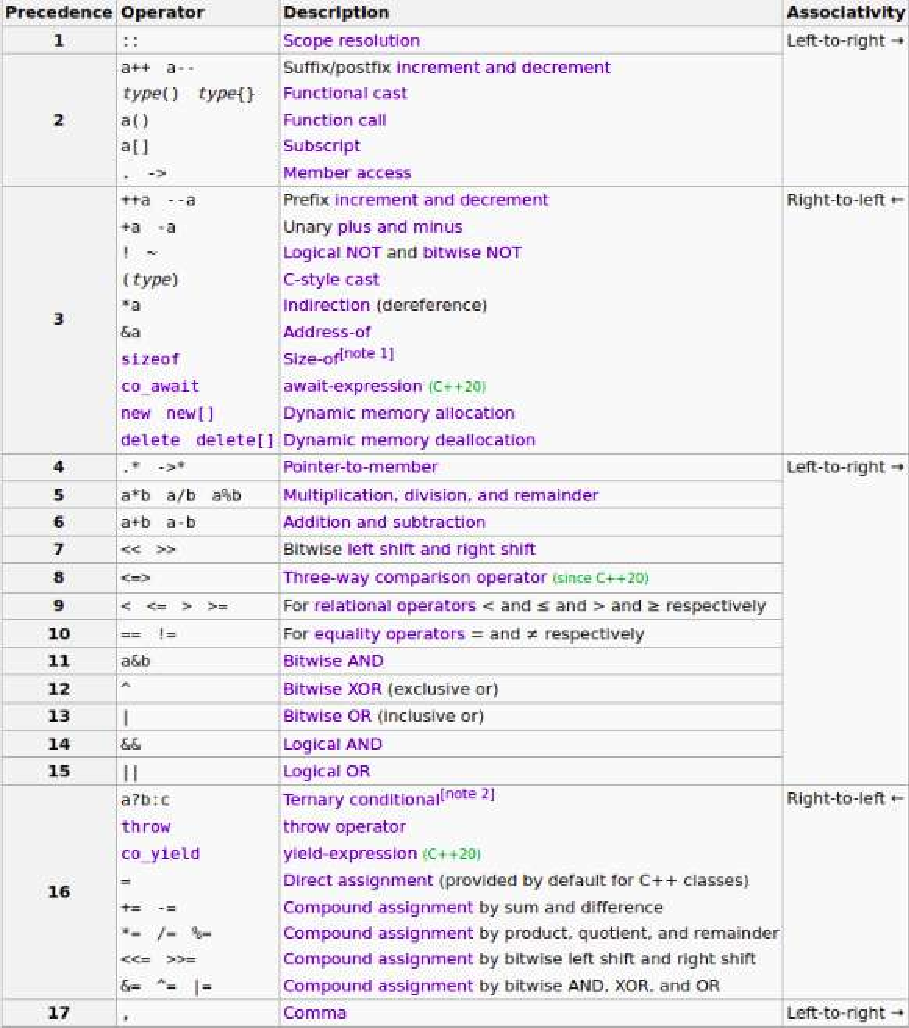
\includepdf[pages=1, scale=0.8]{ops.pdf}
	

تقدم عملگر‌ها با بارگذاری بیش از حد عملگر‌ها (\lr{operator overloading}) تغییری نمی‌کند و ثابت خواهد ماند.
برای نمونه در مثال زیر نحوه ارزیابی مشخص شده است.

\begin{LTR} % Left-to-right environment for code
	\begin{lstlisting}
		cout << a ? b : c;
	\end{lstlisting}
\end{LTR}

\begin{LTR} % Left-to-right environment for code
	\begin{lstlisting}
		(cout << a) ? b : c;
	\end{lstlisting}
\end{LTR}
\section{گرامر بدون ابهام رعایت تقدم عملگر‌ها}

\begin{table}[h!]
	\centering
	\begin{tabular}{|c|c|}
		\hline
		\textbf{عملگرها} & \textbf{تقدم} \\
		\hline
		\texttt{\&\&}, \texttt{||} & 5 \\
		\hline
		\texttt{\&}, \texttt{|} & 4 \\
		\hline
		\texttt{+}, \texttt{-} & 3 \\
		\hline
		\texttt{*}, \texttt{/} & 2 \\
		\hline
		\texttt{a++}, \texttt{a--} & 1 \\
		\hline
	\end{tabular}
	\caption{تقدم عملگرها در زبان C++}
	\label{tab:operator_precedence}
\end{table}

\begin{align*}
	\langle \text{id} \rangle &\to A \mid B \mid C \mid D \mid \dots \\
	\langle \text{assign} \rangle &\to \langle \text{id} \rangle = \langle \text{logical-or} \rangle \\
	\langle \text{logical-or} \rangle &\to \langle \text{logical-or} \rangle \, || \, \langle \text{logical-and} \rangle \mid \langle \text{logical-or} \rangle \\
	\langle \text{logical-and} \rangle &\to \langle \text{logical-and} \rangle \, && \, \langle \text{bitwise-or} \rangle \mid \langle \text{bitwise-or} \rangle \\
	\langle \text{bitwise-or} \rangle &\to \langle \text{bitwise-or} \rangle \, | \, \langle \text{bitwise-and} \rangle \mid \langle \text{bitwise-and} \rangle \\
	\langle \text{bitwise-and} \rangle &\to \langle \text{bitwise-and} \rangle \, \& \, \langle \text{additive} \rangle \mid \langle \text{additive} \rangle \\
	\langle \text{additive} \rangle &\to \langle \text{additive} \rangle \, (+, -) \, \langle \text{multiplicative} \rangle \mid \langle \text{multiplicative} \rangle \\
	\langle \text{multiplicative} \rangle &\to \langle \text{multiplicative} \rangle \, (*, /) \, \langle \text{factor} \rangle \mid \langle \text{factor} \rangle \\
	\langle \text{factor} \rangle &\to (\langle \text{logical-or} \rangle) \mid \langle \text{id} \rangle \mid \langle \text{id} \rangle++ \mid \langle \text{id} \rangle--
\end{align*}
\section{معناشناسی عملیاتی بعضی از ساختارها}

\subsection{تخصیص مقدار به متغیر}
\begin{LTR} % Left-to-right environment for code
	\begin{lstlisting}[breaklines=true]
		x = 5;
		
		MOV R1, #5      ; Load the constant 5 into register R1
		MOV [x], R1     ; Store the value of R1 into memory at
		the address of x
	\end{lstlisting}
\end{LTR}

\subsection{جمع دو مقدار}
\begin{LTR} % Left-to-right environment for code
	\begin{lstlisting}[breaklines=true]
		z = x + y;
		
		MOV R1, [x]     ; Load the value of x into register R1
		MOV R2, [y]     ; Load the value of y into register R2
		ADD R3, R1, R2  ; Add the values in R1 and R2, store 
		the result in R3
		MOV [z], R3     ; Store the result in memory location z
	\end{lstlisting}
\end{LTR}

\subsection{شرط ساده \lr{(if-else)}}
\begin{LTR} % Left-to-right environment for code
	\begin{lstlisting}[breaklines=true]
		if (x > 0) {
			y = 1;
		} else {
			y = -1;
		}
		
		MOV R1, [x]      ; Load x into R1
		CMP R1, #0       ; Compare R1 with 0
		JLE ELSE_LABEL   ; Jump to ELSE_LABEL if R1 <= 0
		MOV [y], #1      ; If x > 0, assign 1 to y
		JMP END_LABEL    ; Skip the else branch
		ELSE_LABEL:
		MOV [y], #-1     ; If x <= 0, assign -1 to y
		END_LABEL:
	\end{lstlisting}
\end{LTR}


\subsection{حلقه \lr{(while)}}
\begin{LTR} % Left-to-right environment for code
	\begin{lstlisting}[breaklines=true]
		while (x > 0) {
			x = x - 1;
		}
		
		
		LOOP_LABEL:
		MOV R1, [x]      ; Load x into R1
		CMP R1, #0       ; Compare R1 with 0
		JLE END_LABEL    ; Exit the loop if R1 <= 0
		SUB R1, R1, #1   ; Decrement R1 by 1
		MOV [x], R1      ; Update x in memory
		JMP LOOP_LABEL   ; Repeat the loop
		END_LABEL:
	\end{lstlisting}
\end{LTR}


\subsection{حلقه \lr{(for)}}
\begin{LTR} % Left-to-right environment for code
	\begin{lstlisting}[breaklines=true]
		for (int i = 0; i < 5; i++) {
			sum = sum + i;
		}
		
		
		; Initialize the loop counter i = 0
		MOV R1, #0        ; Load 0 into R1 (i = 0)
		MOV [i], R1       ; Store the value of i in memory
		
		; Initialize sum = 0
		MOV R2, #0        ; Load 0 into R2 (sum = 0)
		MOV [sum], R2     ; Store the value of sum in memory
		
		FOR_LOOP_START:
		; Compare i with the upper limit (5)
		MOV R1, [i]       ; Load the current value of i into R1
		CMP R1, #5        ; Compare i with 5
		JGE FOR_LOOP_END  ; If i >= 5, jump to end of the loop
		
		; Add i to sum
		MOV R2, [sum]     ; Load the current value of sum into R2
		ADD R2, R2, R1    ; Compute sum + i
		MOV [sum], R2     ; Store the updated sum back into memory
		
		; Increment i by 1
		MOV R1, [i]       ; Load the current value of i into R1
		ADD R1, R1, #1    ; Increment i by 1
		MOV [i], R1       ; Store the updated value of i in memory
		
		; Jump back to the start of the loop
		JMP FOR_LOOP_START
		
		FOR_LOOP_END:
		; End of the loop
	\end{lstlisting}
\end{LTR}


\subsection{تعریف و فراخوانی تابع}
\begin{LTR} % Left-to-right environment for code
	\begin{lstlisting}[breaklines=true]
		int add(int a, int b) {
			return a + b;
		}
		
		int result = add(3, 4);
		
		
		; Define the function
		ADD_FUNC:
		PUSH R1          ; Save registers
		PUSH R2
		ADD R3, R1, R2   ; Compute a + b, store result in R3
		POP R2           ; Restore registers
		POP R1
		RET              ; Return from the function
		
		; Call the function
		MOV R1, #3       ; Pass 3 as the first argument (in R1)
		MOV R2, #4       ; Pass 4 as the second argument (in R2)
		CALL ADD_FUNC    ; Call the add function
		MOV [result], R3 ; Store the result in memory
	\end{lstlisting}
\end{LTR}


\subsection{استراکت}
\begin{LTR} % Left-to-right environment for code
	\begin{lstlisting}[breaklines=true]
		struct Point {
			int x;
			int y;
		};
		
		int main() {
			Point p;
			p.x = 5;
			p.y = 10;
			return 0;
		}
		
		
		main:
		pushq   %rbp                # Save base pointer
		movq    %rsp, %rbp          # Set stack frame
		subq    $16, %rsp           # Allocate 16 bytes on 
		the stack for 'p'
		
		movl    $5, -8(%rbp)        # Set p.x = 5
		movl    $10, -4(%rbp)       # Set p.y = 10
		
		movl    $0, %eax            # Return 0
		leave                       # Restore base pointer
		ret                         # Return
	\end{lstlisting}
\end{LTR}
\chapter{متغیرها و نوع‌های داده‌ای}
\section{انقیاد}

\subsection{انقیاد نوع}
انقیاد نوع به معنی این است که نوع یک متغیر در چه زمانی و چگونه تعیین می‌‌شود. زبان \lr{C++} یک زبان انقیاد نوع ایستا است اما در سناریو‌هایی مانند پلی مورفیسم از انقیاد نوع پویا نیز پشتیبانی می‌کند.

\subsubsection{انقیاد نوع ایستا در \lr{C++}}
\begin{itemize}
	\item نوع متغیر در زمان کامپایل مشخص می‌شود.
	\item خطاهای مرتبط با نوع در زمان کامپایل بررسی می‌شود.
	\item به دلیل تعیین خطاها و تشخیص نوع‌ها در زمان کامپایل زمان اجرا پایین است.
\end{itemize}

زبان C++ روش‌های مختلفی برای استفاده از این نوع تعریف کرده است:
\begin{itemize}
	\item تعریف متغیر‌ها در برنامه
	\begin{LTR} % Left-to-right environment for code
		\begin{lstlisting}[breaklines=true]
			int num = 10;        // `num` is bound to type 
			`// int` at compile-time.
			double pi = 3.14;    // `pi` is bound to type 
			`// double` at compile-time.
			char ch = 'A';       // `ch` is bound to type `
			// char` at compile-time.
		\end{lstlisting}
	\end{LTR}
	
	
	\item تعریف توابع عادی در برنامه
	\begin{LTR} % Left-to-right environment for code
		\begin{lstlisting}[breaklines=true]
			void print(int value) {
				std::cout << "Integer: " << value << std::endl;
			}
			
			void print(double value) {
				std::cout << "Double: " << value << std::endl;
			}
			
			void print(const char* value) {
				std::cout << "String: " << value << std::endl;
			}
			
			int main() {
				print(10);               // Resolves to print(int)
				print(3.14);             // Resolves to print(double)
				print("Hello World");    // Resolves to print(const char*)
				return 0;
			}
		\end{lstlisting}
	\end{LTR}
	
	
	\item بارگذاری عملگرها
	\begin{LTR} % Left-to-right environment for code
		\begin{lstlisting}[breaklines=true]
			class Complex {
				public:
				double real, imag;
				
				Complex(double r, double i) : real(r), imag(i) {}
				
				Complex operator+(const Complex& c) {
					return Complex(real + c.real, imag + c.imag);
				}
			};
			
			int main() {
				Complex c1(1.0, 2.0), c2(3.0, 4.0);
				Complex c3 = c1 + c2;    // Operator `+` resolved at compile-time
				
				std::cout << "Real: " << c3.real << ", Imaginary: " << c3.imag << std::endl;
				return 0;
			}
			
		\end{lstlisting}
	\end{LTR}
	
	
	\item قالب‌های توابع (\lr{Function Templates})
	\begin{LTR} % Left-to-right environment for code
		\begin{lstlisting}[breaklines=true]
			template <typename T>
			T add(T a, T b) {
				return a + b;
			}
			
			int main() {
				std::cout << add(3, 4) << std::endl;         // Instantiates add<int>
				std::cout << add(3.14, 1.86) << std::endl;  // Instantiates add<double>
				return 0;
			}
		\end{lstlisting}
	\end{LTR}
	
	
	\item توابع خطی (\lr{inline})
	\begin{LTR} % Left-to-right environment for code
		\begin{lstlisting}[breaklines=true]
			inline int square(int x) {
				return x * x;
			}
			
			int main() {
				std::cout << square(5) << std::endl;   // `square(5)` is replaced with `5 * 5` at compile-time
				return 0;
			}
		\end{lstlisting}
	\end{LTR}
	
	
	\item عبارات ثابت
	\begin{LTR} % Left-to-right environment for code
		\begin{lstlisting}[breaklines=true]
			constexpr int square(int x) {
				return x * x;
			}
			
			int main() {
				constexpr int result = square(5);  // Computed at compile-time
				std::cout << result << std::endl;
				return 0;
			}
		\end{lstlisting}
	\end{LTR}
	
	
	
	\item توابع کلاس‌ها
	\begin{LTR} % Left-to-right environment for code
		\begin{lstlisting}[breaklines=true]
			class Base {
				public:
				void display() {
					std::cout << "Base class display" << std::endl;
				}
			};
			
			class Derived : public Base {
				public:
				void display() {
					std::cout << "Derived class display" << std::endl;
				}
			};
			
			int main() {
				Base obj;
				obj.display();   // Resolves to Base::display() at compile-time
				return 0;
			}
		\end{lstlisting}
	\end{LTR}
	
	\item عبارت‌های لامبدا
	\begin{LTR} % Left-to-right environment for code
		\begin{lstlisting}[breaklines=true]
			int main() {
				auto add = [](int a, int b) { return a + b; };  // Resolved at compile-time
				std::cout << add(3, 4) << std::endl;
				return 0;
			}
		\end{lstlisting}
	\end{LTR}
	
\end{itemize}


\subsubsection{انقیاد نوع پویا در \lr{C++}}
\begin{itemize}
	\item نوع متغیر در زمان اجرا مشخص می‌شود.
	\item خطاهای مرتبط با نوع در زمان اجرا بررسی می‌شود.
	\item به دلیل تعیین خطاها و تشخیص نوع‌ها در زمان اجرا زمان اجرا بالا است.
\end{itemize}

زبان \lr{C++} به دلیل زمان اجرای پایین این نوع انقیاد روش‌ محدودی را برای استفاده از این نوع تعریف کرده است و آن هم استفاده از توابع مجازی است.

\begin{LTR} % Left-to-right environment for code
	\begin{lstlisting}[breaklines=true]
		class Base {
			public:
			virtual void display() {  // Virtual function enables dynamic binding
				std::cout << "Base class display" << std::endl;
			}
		};
		
		class Derived : public Base {
			public:
			void display() override {  // Overrides the base class method
				std::cout << "Derived class display" << std::endl;
			}
		};
		
		int main() {
			Base* basePtr;
			Derived derivedObj;
			basePtr = &derivedObj;
			
			basePtr->display();  // Resolved at runtime to Derived::display
			return 0;
		}
	\end{lstlisting}
\end{LTR}


\begin{LTR} % Left-to-right environment for code
	\begin{lstlisting}[breaklines=true]
		class Animal {
			public:
			virtual void speak() = 0;  // Pure virtual function
		};
		
		class Dog : public Animal {
			public:
			void speak() override {
				std::cout << "Woof!" << std::endl;
			}
		};
		
		class Cat : public Animal {
			public:
			void speak() override {
				std::cout << "Meow!" << std::endl;
			}
		};
		
		int main() {
			Animal* animal;
			
			Dog dog;
			Cat cat;
			
			animal = &dog;
			animal->speak();  // Resolved at runtime to Dog::speak
			
			animal = &cat;
			animal->speak();  // Resolved at runtime to Cat::speak
			
			return 0;
		}
	\end{lstlisting}
\end{LTR}
\section{مقایسه انقیاد ایستا و پویا}

\begin{table}[h!]
	\centering
	\begin{tabular}{|p{3cm}|p{5cm}|p{5cm}|}
		\hline
		\textbf{ویژگی} & \textbf{انقیاد ایستا} & \textbf{انقیاد پویا} \\
		\hline
		زمان حل اتصال & زمان کامپایل & زمان اجرا \\
		\hline
		عملکرد & بالا (بدون سربار در زمان اجرا) & کمی کندتر (سربار جدول مجازی و\lr{ RTTI}) \\
		\hline
		تشخیص خطا & در زمان کامپایل (ایمن‌تر) & در زمان اجرا (کمتر ایمن) \\
		\hline
		انعطاف‌پذیری & محدود (نوع‌ها در زمان کامپایل ثابت هستند) & بالا (پشتیبانی از چندریختی در زمان اجرا) \\
		\hline
		قابلیت گسترش & نیاز به بازکامپایل برای تغییرات & راحت برای گسترش (مثلاً اضافه کردن کلاس‌های جدید) \\
		\hline
		سهولت در دیباگ & آسان‌تر (رفتار قابل پیش‌بینی است) & دشوارتر (رفتار وابسته به زمان اجرا است) \\
		\hline
		استفاده از حافظه & کم (نیاز به فراداده اضافی نیست) & بیشتر (نیاز به جدول مجازی و \lr{RTTI}) \\
		\hline
		موارد استفاده & کدهای کارآمد و قابل پیش‌بینی (مثل الگوریتم‌ها) & طراحی انعطاف‌پذیر و قابل گسترش (مثل فریم‌ورک‌ها) \\
		\hline
	\end{tabular}
	\caption{مقایسه انقیاد ایستا و پویا}
	\label{tab:static_dynamic_binding}
\end{table}

\subsection{انقیاد مقدار یا حافظه}
انقیاد مقدار به معنی این است که نوع یک متغیر در چه زمانی و چگونه به حافظه مقید می‌‌شود. 
زبان\lr{ C++} از انواع زیر پشتیبانی می‌کند:


\subsubsection{انقیاد در زمان کامپایل}
\begin{itemize}
	\item آدرس حافظه در زمان کامپایل تعیین می‌شود.
	\item این نوع انقیاد در زبان \lr{C++ }مرسوم‌‌تر است و برای متغیر‌های محلی و سراسری و ایستا استفاده می‌شود.
	
	\begin{LTR} % Left-to-right environment for code
		\begin{lstlisting}[breaklines=true]
			int x = 10;
			static int y = 0;
		\end{lstlisting}
	\end{LTR}
\end{itemize}


\subsubsection{انقیاد در زمان اجرا}
\begin{itemize}
	\item آدرس حافظه در زمان اجرا مشخص می‌شود.
	\item برنامه‌نویس مسئول آزاد کردن حافظه است.
	\item این نوع انقیاد معمولاً در تخصیص پویا (\lr{Dynamic Allocation}) با استفاده از دستوراتی مانند \lr{new} انجام می‌شود.
	
	
	\begin{LTR} % Left-to-right environment for code
		\begin{lstlisting}
			int* ptr = new int(10);
		\end{lstlisting}
	\end{LTR}
\end{itemize}


\subsubsection{انقیاد موقت}
\begin{itemize}
	\item حافظه به صورت موقت رزرو می‌شود.
	\item این نوع انقیاد زمانی رخ می‌دهد که یک مقدار موقت (\lr{temporary}) به یک مرجع متصل شود. این اتصال تا زمانی که مرجع در محدوده است، معتبر باقی می‌ماند.
	
	
	\begin{LTR} % Left-to-right environment for code
		\begin{lstlisting}
			const int& ref = 42;
		\end{lstlisting}
	\end{LTR}
\end{itemize}


\subsubsection{انقیاد پویا با اشاره‌گرهای هوشمند}
\begin{itemize}
	\item آزادسازی حافظه به صورت خودکار توسط اشاره‌گر هوشمند انجام می‌شود.
	\item در \lr{C++} مدرن (11 به بعد)، از اشاره‌گرهای هوشمند برای مدیریت انقیاد حافظه به صورت خودکار استفاده می‌شود.
\end{itemize}

\begin{LTR} % Left-to-right environment for code
	\begin{lstlisting}[breaklines=true]
		std::unique_ptr<int> ptr = std::make_unique<int>(10);
	\end{lstlisting}
\end{LTR}


\section{تعریف متغیر}
در زبان \lr{C++ }تعریف متغیر صریح مرسوم است اما ابزاری برای تعریف متغیر ضمنی نیز وجود دارد.

\subsection{تعریف متغیر صریح}
نوع متغیر به‌طور واضح و صریح در هنگام تعریف مشخص می‌شود.

\begin{LTR} % Left-to-right environment for code
	\begin{lstlisting}[breaklines=true]
		int age = 25;          // 'age' is explicitly defined as an integer.
		double pi = 3.14;      // 'pi' is explicitly defined as a double.
		string name = "John";  // 'name' is explicitly defined as a string.
	\end{lstlisting}
\end{LTR}

\subsection{تعریف متغیر ضمنی}
نوع متغیر برابر با \lr{auto} قرار می‌گیرد و نوع به‌طور خودکار توسط کامپایلر با توجه به مقدار زمینه تعیین می‌شود.

\begin{LTR} % Left-to-right environment for code
	\begin{lstlisting}[breaklines=true]
		auto age = 25;         // The type of 'age' is inferred as int.
		auto pi = 3.14;        // The type of 'pi' is inferred as double.
		auto name = "John";    // The type of 'name' is inferred as const char*.
	\end{lstlisting}
\end{LTR}

\begin{table}[h!]
	\centering
	\begin{tabular}{|p{3cm}|p{5cm}|p{5cm}|}
		\hline
		\textbf{ویژگی} & \textbf{تعریف صریح} & \textbf{تعریف ضمنی} \\
		\hline
		وضوح & 
		نوع متغیر به‌طور واضح و مستقیم مشخص می‌شود. & 
		نوع متغیر توسط کامپایلر استنباط می‌شود و ممکن است بلافاصله واضح نباشد. \\
		\hline
		انعطاف‌پذیری & 
		نیاز به دانستن نوع متغیر قبل از تعریف دارد. & 
		می‌تواند براساس مقدار داده شده، نوع را تطبیق دهد. \\
		\hline
		نحو (\lr{Syntax}) & 
		روش سنتی و نسبتاً طولانی. & 
		کوتاه‌تر و مدرن‌تر با استفاده از \texttt{\lr{auto}}. \\
		\hline
		مورد استفاده & 
		مناسب برای مواردی که وضوح و کنترل اهمیت دارند. & 
		مناسب برای کاهش کد تکراری، مخصوصاً در انواع پیچیده. \\
		\hline
	\end{tabular}
	\caption{مقایسه تعریف صریح و تعریف ضمنی متغیرها در زبان C++}
	\label{tab:explicit_implicit}
\end{table}


\section{متغیرهای ایستا}

\subsection{متغیرهای ایستا در توابع}
\begin{itemize}
	\item مقدار آن بین فراخوانی‌های مختلف تابع حفظ می‌شود.
	\item فقط یک بار مقداردهی اولیه می‌شود.
	\item مقدار آن پس از خروج از تابع باقی می‌ماند.
	\item دامنه (\lr{Scope}) متغیر همچنان محدود به تابع است، اما طول عمر (\lr{Lifetime}) آن برابر با طول عمر برنامه خواهد بود.
	\item در قسمت دیتا سگمنت ذخیره می‌شود.
\end{itemize}


\begin{LTR} % Left-to-right environment for code
	\begin{lstlisting}[breaklines=true]
		void countCalls() {
			static int count = 0; // متغیر استاتیک
			count++;
			cout << "This function has been called " << count << " times." << endl;
		}
		
		int main() {
			countCalls();
			countCalls();
			countCalls();
			return 0;
		}
	\end{lstlisting}
\end{LTR}

خروجی:

\begin{LTR} % Left-to-right environment for code
	\begin{lstlisting}[breaklines=true]
		This function has been called 1 times.
		This function has been called 2 times.
		This function has been called 3 times.
	\end{lstlisting}
\end{LTR}


\subsection{متغیرهای ایستا در کلاس‌ها}
\begin{itemize}
	\item در داخل یک کلاس، متغیرهای استاتیک به همه اشیاء (\lr{Objects}) آن کلاس مشترک هستند. این متغیرها بخشی از فضای ذخیره‌سازی کلاس هستند، نه اشیاء جداگانه.
	\item مستقل از اشیاء کلاس هستند.
	\item فقط یک نسخه از آنها در حافظه وجود دارد که توسط تمام اشیاء به اشتراک گذاشته می‌شود.
	\item برای دسترسی به آنها می‌توان از نام کلاس استفاده کرد.
	\item در قسمت دیتا سگمنت ذخیره می‌شود.
\end{itemize}


\begin{LTR} % Left-to-right environment for code
	\begin{lstlisting}[breaklines=true]
		class Counter {
			private:
			static int count; // متغیر استاتیک
			public:
			Counter() {
				count++;
			}
			static void showCount() { // متد استاتیک
				cout << "Count: " << count << endl;
			}
		};
		
		int Counter::count = 0; // مقداردهی اولیه متغیر استاتیک
		
		int main() {
			Counter c1, c2, c3;
			Counter::showCount(); // دسترسی به متغیر استاتیک از طریق کلاس
			return 0;
		}
	\end{lstlisting}
\end{LTR}

خروجی:

\begin{LTR} % Left-to-right environment for code
	\begin{lstlisting}[breaklines=true]
		Count: 3
	\end{lstlisting}
\end{LTR}

\subsubsection{مزایا}
\begin{itemize}
	\item حفظ مقدار متغیر در توابع بدون نیاز به استفاده از متغیرهای سراسری.
	\item صرفه‌جویی در حافظه برای متغیرهای مشترک در بین اشیاء کلاس.
	\item امکان پیاده‌سازی شمارنده‌ها، حافظه پنهان (\lr{Cache}) و بسیاری از موارد دیگر.
\end{itemize}


\section{پویا در پشته}

\subsection{متغیر‌های محلی}
هنگام اجرای تابع حافظه تخصیص داده می‌شود و در پایان تابع آزاد می‌‌شوند.



\begin{LTR} % Left-to-right environment for code
	\begin{lstlisting}[breaklines=true]
		void myFunction() {
			int a = 10;  // Stored on the stack
		}
	\end{lstlisting}
\end{LTR}


\subsection{پارامتر‌های توابع}


\begin{LTR} % Left-to-right environment for code
	\begin{lstlisting}[breaklines=true]
		void printNumber(int num) {
			// num is stored on the stack
		}
	\end{lstlisting}
\end{LTR}

\subsubsection{آرایه‌‌های محلی غیر پویا}
\begin{LTR} % Left-to-right environment for code
	\begin{lstlisting}[breaklines=true]
		void myFunction() {
			int arr[5] = {1, 2, 3, 4, 5}; // روی پشته ذخیره می‌شود
		}
	\end{lstlisting}
\end{LTR}


\section{متغیرهای پویا در هیپ به طور صریح}

زبان C++ تعریف این متغیرها را ممکن ساخته است و برای این کار از دو عملگر \lr{new} (برای تخصیص حافظه) و عملگر \lr{delete} (برای آزاد کردن فضای تخصیص داده‌ شده) استفاده می‌کند.

\begin{itemize}
	\item حافظه‌ای که با new تخصیص داده شده باید حتماً با delete آزاد شود.
	\item آزاد نکردن حافظه منجر به نشت حافظه (\lr{memory leak}) می‌شود.
	\item استفاده از \lr{delete} برای حافظه‌ای که تخصیص نیافته یا قبلاً آزاد شده است، باعث رفتار غیرقابل پیش‌بینی خواهد شد.
\end{itemize}


\begin{LTR} % Left-to-right environment for code
	\begin{lstlisting}[breaklines=true]
		int* ptr = new int;
		int* arr = new int[5];
		Data* data = new Data(); // instance of class Data
	\end{lstlisting}
\end{LTR}


\section{متغیرهای پویا در هیپ به طور ضمنی}

زبان \lr{C++} امکان استفاده از این نوع متغیرها را نیز فراهم کرده است و از طریق اشاره‌گر‌های هوشمند و یا کتاب‌خانه‌های استاندارد و … از این روش استفاده می‌کند. همچنین در این روش متغیر‌ها در بخش هیپ ذخیره می‌شوند اما ابزار‌های آماده حافظه را به‌‌صورت خودکار مدیریت می‌‌‌کنند.


\subsection{اشاره‌گرهای هوشمند}


\begin{LTR} % Left-to-right environment for code
	\begin{lstlisting}[breaklines=true]
		#include <memory> // For smart pointers
		
		int main() {
			// Define a shared_ptr to manage a dynamic integer
			std::shared_ptr<int> ptr = std::make_shared<int>(42);
			
			std::cout << "Value: " << *ptr << std::endl;
			
			// Memory is automatically freed when it goes out of scope
			
			return 0;
		}
	\end{lstlisting}
\end{LTR}

\subsubsection{کانتینرهای STL}
\begin{LTR} % Left-to-right environment for code
	\begin{lstlisting}[breaklines=true]
		#include <vector>
		
		int main() {
			// Define a vector of integers
			std::vector<int> numbers = {1, 2, 3, 4, 5};
			
			// Add an element to the vector
			numbers.push_back(6);
			
			// Print the values of the vector
			for (int num : numbers) {
				std::cout << num << " ";
			}
			std::cout << std::endl;
			
			// No need to free memory; it is managed automatically
			
			return 0;
		}
	\end{lstlisting}
\end{LTR}


\begin{table}[h!]
	\centering
	\begin{tabular}{|p{4cm}|p{6cm}|p{6cm}|}
		\hline
		\textbf{نوع متغیر} & \textbf{مزایا} & \textbf{معایب} \\
		\hline
		ایستا &
		\begin{itemize}
			\item تخصیص حافظه ثابت در طول عمر برنامه.
			\item حفظ مقدار بین اجرای توابع.
			\item بدون سربار حافظه در زمان اجرا.
		\end{itemize} &
		\begin{itemize}
			\item حافظه در طول عمر برنامه اشغال می‌شود، حتی اگر به ندرت استفاده شود.
			\item ممکن است باعث افزایش غیرضروری حافظه شود.
		\end{itemize} \\
		\hline
		پویا در پشته &
		\begin{itemize}
			\item مناسب برای مقادیر ثابت یا مقادیری که به ندرت تغییر می‌کنند.
			\item تخصیص و آزادسازی خودکار (بر اساس محدوده متغیر).
			\item تخصیص و آزادسازی سریع (روی پشته).
			\item امنیت بالا.
		\end{itemize} &
		\begin{itemize}
			\item نمی‌توانند خارج از محدوده تابع باقی بمانند.
		\end{itemize} \\
		\hline
		پویا در هیپ به طور صریح &
		\begin{itemize}
			\item انعطاف‌پذیری: اندازه حافظه در زمان اجرا تعیین می‌شود.
			\item مناسب برای داده‌های بزرگ و پویا.
			\item کنترل دستی بر طول عمر حافظه فراهم می‌کند.
		\end{itemize} &
		\begin{itemize}
			\item نیازمند تخصیص دستی (\texttt{new}) و آزادسازی دستی (\texttt{delete}).
			\item احتمال نشت حافظه در صورت آزاد نکردن صحیح.
			\item خطر رفتار غیرقابل پیش‌بینی در صورت آزادسازی دوباره یا دسترسی پس از آزادسازی.
		\end{itemize} \\
		\hline
		پویا در هیپ به طور ضمنی &
		\begin{itemize}
			\item مدیریت خودکار حافظه (مانند کانتینرهای STL یا اشاره‌گرهای هوشمند).
			\item کاهش خطر نشت حافظه و رفتار غیرقابل پیش‌بینی.
			\item ساده کردن برنامه‌نویسی برای مفاهیم سطح بالا.
		\end{itemize} &
		\begin{itemize}
			\item کمی سربار عملکرد به دلیل مدیریت خودکار حافظه.
			\item کنترل کمتری بر تخصیص و آزادسازی حافظه.
			\item ممکن است در برنامه‌های حساس به عملکرد که هر تخصیص اهمیت دارد، بهینه نباشد.
		\end{itemize} \\
		\hline
	\end{tabular}
	\caption{مقایسه روش‌های تخصیص حافظه}
	\label{tab:memory_allocation}
\end{table}

\subsection{مقایسه سرعت انواع متغیرها}
\begin{table}[H]
	\centering
	\begin{tabular}{|p{4cm}|p{3cm}|p{7cm}|}
		\hline
		\textbf{نوع متغیر} & \textbf{سرعت} & \textbf{دلیل} \\
		\hline
		ایستا &
		بدون هزینه در زمان اجرا &
		این متغیرها در زمان کامپایل و در یک منطقه ثابت حافظه تخصیص داده می‌شوند. نیازی به جستجو یا نگهداری در زمان اجرا نیست. \\
		\hline
		پویا در پشته &
		سریع‌ترین &
		تخصیص در استک یک فرآیند ساده است که فقط اشاره‌گر حافظه را افزایش یا کاهش می‌دهد. نیازی به نگهداری پیچیده نیست. \\
		\hline
		پویا در هیپ به طور صریح &
		کندترین &
		هیپ یک فضای حافظه بزرگ و نامرتب است که نیاز به نگهداری پیچیده‌ای دارد. سیستم‌عامل یا زمان اجرا باید یک بلوک آزاد مناسب برای تخصیص پیدا کند. سربار شامل جستجوی حافظه، به‌روزرسانی ساختارهای داده داخلی و تضمین ایمنی رشته‌ها است. \\
		\hline
		پویا در هیپ به طور ضمنی &
		متوسط &
		حافظه هنوز روی هیپ تخصیص داده می‌شود، اما زمان اجرا از تکنیک‌هایی مانند اشاره‌گرهای ساده یا مجموعه‌های حافظه استفاده می‌کند. این فرآیند از تخصیص صریح کمی سریع‌تر است چون برنامه به طور مستقیم با توابع تخصیص سطح پایین درگیر نمی‌شود. فرآیند جمع‌آوری زباله (\lr{garbage collection}) سربار اضافی در آینده ایجاد می‌کند. \\
		\hline
	\end{tabular}
	\caption{مقایسه سرعت و دلایل تخصیص حافظه}
	\label{tab:memory_speed}
\end{table}
\pagebreak
\section{حوزه تعریف }
\subsection{حوزه تعریف ایستا \lr{(Static Scope)} در \lr{C++}}
در \lr{C++}، هر متغیر یا تابع در حوزه‌ای خاص تعریف می‌شود و دسترسی به آن‌ها از خارج از آن حوزه امکان‌پذیر نیست. این حوزه‌ها معمولاً در زمان کامپایل مشخص می‌شوند و شامل دو نوع اصلی هستند:

\subsubsection{حوزه تعریف درون توابع \lr{(Local Scope)}}
متغیرهایی که در داخل توابع یا بلوک‌ها تعریف می‌شوند، تنها در آن تابع یا بلوک قابل دسترسی هستند. این نوع متغیرها در زمان اجرای برنامه تنها در محدوده‌ای که تعریف شده‌اند معتبر هستند و پس از خروج از آن حوزه از بین می‌روند.

\textbf{مثال 1: متغیر محلی در یک تابع}
\LTR
\begin{lstlisting}[language=C++,breaklines=true]
	#include <iostream>
	
	void exampleFunction() {
		int x = 10; // access just here
		std::cout << "x = " << x << std::endl;
	}
	
	int main() {
		exampleFunction();
		// std::cout << x;  // error
		return 0;
	}
\end{lstlisting}
\RTL

در این مثال، متغیر \lr{x} تنها درون تابع \lr{exampleFunction} تعریف شده است و دسترسی به آن از خارج از تابع مجاز نیست.

\subsubsection{حوزه تعریف سراسری \lr{(Global Scope)}}
متغیرهایی که خارج از توابع و کلاس‌ها، در سطح کل برنامه تعریف می‌شوند، در تمام برنامه قابل دسترسی هستند. این متغیرها معمولاً از نوع \lr{global} هستند و در تمامی توابع یا کلاس‌ها می‌توانند استفاده شوند (به شرطی که در ابتدای برنامه تعریف شده باشند).

\textbf{مثال 2: متغیر سراسری}
\LTR
\begin{lstlisting}[language=C++, breaklines=true]
	#include <iostream>
	
	int globalVar = 5; // global
	
	void printGlobalVar() {
		std::cout << "globalVar = " << globalVar << std::endl; // access to global
	}
	
	int main() {
		printGlobalVar();
		return 0;
	}
\end{lstlisting}
\RTL

در این مثال، متغیر \lr{globalVar} در سطح سراسری برنامه تعریف شده است و می‌توان به آن از هر کجای برنامه مانند تابع \lr{printGlobalVar} دسترسی پیدا کرد.

\subsubsection{حوزه تعریف درون کلاس‌ها \lr{(Class Scope)}}
در \lr{C++}، متغیرها و توابعی که درون کلاس‌ها تعریف می‌شوند، تنها درون همان کلاس و از طریق شیءهای کلاس قابل دسترسی هستند.

\textbf{مثال 3: متغیر و تابع در کلاس}
\LTR
\begin{lstlisting}[language=C++, breaklines=true]
	#include <iostream>
	
	class MyClass {
		public:
		int value; /
		
		void printValue() { 
			std::cout << "value = " << value << std::endl;
		}
	};
	
	int main() {
		MyClass obj;
		obj.value = 10;
		obj.printValue(); 
		return 0;
	}
\end{lstlisting}
\RTL
در اینجا، متغیر \lr{value} و تابع \lr{printValue} درون کلاس \lr{MyClass} قرار دارند و تنها از طریق اشیاء این کلاس قابل دسترسی هستند.

\section{چالش‌ها و پیاده‌سازی حوزه تعریف پویا در \lr{C++}}
برای شبیه‌سازی حوزه تعریف پویا، نیاز است که متغیرهایی ایجاد شوند که بتوانند از توابع یا بلوک‌های مختلف و به‌صورت دینامیک قابل دسترسی باشند.

\textbf{مثال 1: پیاده‌سازی ساده با متغیر سراسری}
\LTR
\begin{lstlisting}[language=C++, breaklines=true]
#include <iostream>

int dynamicVar = 10;  // Global variable to simulate dynamic scoping

// First function that modifies the value of dynamicVar
void functionOne() {
	dynamicVar = 20;  // Modifying the value of dynamicVar in this function
	std::cout << "functionOne: dynamicVar = " << dynamicVar << std::endl;
}

// Second function that uses dynamicVar
void functionTwo() {
	std::cout << "functionTwo: dynamicVar = " << dynamicVar << std::endl;
}

int main() {
	std::cout << "main: dynamicVar = " << dynamicVar << std::endl;
	functionOne();  // Here, the value of dynamicVar is modified
	functionTwo();  // Here, the modified value of dynamicVar is displayed
	return 0;
}

\end{lstlisting}
\RTL

\textbf{خروجی برنامه:}
\LTR
\begin{verbatim}
	main: dynamicVar = 10
	functionOne: dynamicVar = 20
	functionTwo: dynamicVar = 20
\end{verbatim}
\RTL
در این مثال:
\begin{itemize}
	\item متغیر \lr{dynamicVar} که به‌طور سراسری تعریف شده است، ابتدا در تابع \lr{main} مقداردهی می‌شود.
	\item سپس در تابع \lr{functionOne}، مقدار آن به ۲۰ تغییر می‌کند.
	\item هنگامی که تابع \lr{functionTwo} فراخوانی می‌شود، مقدار تغییر یافته \lr{dynamicVar} نمایش داده می‌شود.
\end{itemize}
\subsection{استفاده از پشته (Stack) برای شبیه‌سازی حوزه پویا}
برای پیاده‌سازی واقعی‌تر حوزه پویا می‌توان از ساختارهای داده‌ای مانند پشته (\lr{stack}) استفاده کرد. این روش اجازه می‌دهد که مقادیر به صورت داینامیک ذخیره شوند و به ترتیب وارد و خارج شوند. به این ترتیب، متغیرها می‌توانند به طور پویا ذخیره و بازیابی شوند.

\textbf{مثال 2: استفاده از پشته برای ذخیره و بازیابی مقادیر}
\LTR
\begin{lstlisting}[language=C++,  breaklines=true]
	#include <iostream>
	#include <stack>
	
	// Stack to store variable values
	std::stack<int> dynamicStack;
	
	// Function to push a new value to the stack
	void functionOne() {
		dynamicStack.push(30);  // Add a new value to the stack
		std::cout << "functionOne: pushed 30" << std::endl;
	}
	// Function to retrieve the top value from the stack
	void functionTwo() {
		if (!dynamicStack.empty()) {
			int topValue = dynamicStack.top();  // Get the top value of the stack
			std::cout << "functionTwo: top of stack = " << topValue << std::endl;
			dynamicStack.pop();  // Remove the top value from the stack
		}
	}
	int main() {
		std::cout << "main: Initial stack is empty" << std::endl;
		functionOne();  // Add a new value to the stack
		functionTwo();  // Display the top value and remove it from the stack
		return 0;
	}
\end{lstlisting}
\RTL
\textbf{خروجی برنامه:}
\LTR
\begin{verbatim}
	main: Initial stack is empty
	functionOne: pushed 30
	functionTwo: top of stack = 30
\end{verbatim}
\RTL
در این مثال:
\begin{itemize}
	\item از پشته‌ای به نام \lr{dynamicStack} برای ذخیره مقادیر استفاده شده است.
	\item تابع \lr{functionOne} مقدار ۳۰ را به پشته اضافه می‌کند.
	\item تابع \lr{functionTwo} مقدار بالای پشته را خوانده و آن را از پشته برمی‌دارد.
\end{itemize}


\textbf{نتیجه‌گیری} \\
برای اضافه کردن حوزه تعریف پویا به زبان‌های ایستا مانند \lr{C++}، می‌توان از مکانیزم‌های مختلفی مانند متغیرهای سراسری یا ساختارهای داده‌ای دینامیک (مانند پشته) استفاده کرد. در این پیاده‌سازی، متغیرها می‌توانند در نقاط مختلف برنامه تغییر یافته و از هر کجا به آن‌ها دسترسی پیدا کرد، مشابه رفتار حوزه پویا که در زبان‌هایی مانند \lr{Lisp} مشاهده می‌شود.

\section{بلوک‌ها}
در زبان \lr{C++}، بلوک‌ها (\lr{Blocks}) معمولاً به عنوان مجموعه‌ای از دستورات محصور در آکولادها {} تعریف می‌شوند. این بلوک‌ها می‌توانند به‌عنوان بدنه‌ی توابع، حلقه‌ها، شروط و سایر ساختارهای کنترلی استفاده شوند. در این زبان، کلمات کلیدی خاصی برای تغییر حوزۀ تعریف متغیرها به‌طور مستقیم وجود ندارد، اما برای مدیریت دسترسی و تغییر حوزۀ متغیرها می‌توان از ویژگی‌های مختلف زبان مانند حوزه‌های محلی، حوزه‌های سراسری، و حوزه‌های ثابت بهره برد.

\subsection{تعریف بلوک‌ها در C++}
یک بلوک در \lr{C++} معمولاً به‌صورت مجموعه‌ای از دستورات نوشته می‌شود که بین آکولادها قرار دارند. بلوک‌ها می‌توانند در موقعیت‌های مختلفی قرار بگیرند، از جمله در داخل توابع، حلقه‌ها، و ساختارهای کنترلی مانند \lr{if} یا \lr{for}.

\textbf{مثال 1: تعریف بلوک در داخل یک تابع}
\LTR
\begin{lstlisting}[language=C++, breaklines=true]
	#include <iostream>
	
	void exampleFunction() {
		int x = 10;  // Variable x defined in this block
		{
			int y = 20;  // Variable y defined in this inner block
			std::cout << "Inside inner block: x = " << x << ", y = " << y << std::endl;
		}
		// std::cout << "y = " << y << std::endl; // Error: y is out of scope
	}
	
	int main() {
		exampleFunction();
		return 0;
	}
\end{lstlisting}
\RTL
در این مثال:
\begin{itemize}
	\item تابع \lr{exampleFunction} حاوی یک بلوک داخلی است که در داخل آن متغیر \lr{y} تعریف شده است. این متغیر تنها در داخل بلوک داخلی قابل دسترسی است.
	\item متغیر \lr{x} در داخل بلوک اصلی تابع تعریف شده و در داخل بلوک داخلی هم قابل دسترسی است.
\end{itemize}

\subsection{کلمات کلیدی ویژه برای اعمال تغییر در حوزه تعریف متغیرها}
در \lr{C++}، کلمات کلیدی خاصی برای تغییر مستقیم حوزه تعریف متغیرها وجود ندارد. اما چند ویژگی و کلمه کلیدی می‌توانند برای مدیریت دسترسی و کنترل حوزه متغیرها استفاده شوند:

\subsubsection{ \lr{auto}}
کلمه کلیدی \lr{auto} به کامپایلر این امکان را می‌دهد که نوع یک متغیر را به‌طور خودکار از مقدار آن استنتاج کند. این ویژگی به ساده‌سازی مدیریت حوزه متغیرها کمک می‌کند.

\textbf{مثال 2: استفاده از \lr{auto}}
\LTR
\begin{lstlisting}[language=C++, breaklines=true]
	#include <iostream>
	
	int main() {
		auto x = 5;  // Compiler infers x as int
		auto y = 10.5;  // Compiler infers y as double
		std::cout << "x = " << x << ", y = " << y << std::endl;
		return 0;
	}
\end{lstlisting}
\RTL

\subsubsection{ \lr{static}}
کلمه کلیدی \lr{static} برای حفظ مقدار متغیرها در تمام طول برنامه استفاده می‌شود. متغیرهای \lr{static} بین فراخوانی‌های متعدد یک تابع حفظ می‌شوند.

\textbf{مثال 3: استفاده از \lr{static}}
\LTR
\begin{lstlisting}[language=C++, breaklines=true]
	#include <iostream>
	
	void countCalls() {
		static int count = 0;  // Variable count persists across calls
		count++;
		std::cout << "Function called " << count << " times." << std::endl;
	}
	
	int main() {
		countCalls();
		countCalls();
		countCalls();
		return 0;
	}
\end{lstlisting}
\RTL
\subsubsection{\lr{extern}}
کلمه کلیدی \lr{extern} برای دسترسی به متغیرها یا توابع از فایل‌ها یا بخش‌های دیگر برنامه استفاده می‌شود. این کلمه امکان تعریف متغیرهای سراسری بین فایل‌ها را فراهم می‌کند.

\textbf{مثال 4: استفاده از \lr{extern}}
\LTR
\begin{lstlisting}[language=C++, breaklines=true]
	// File1.cpp
	#include <iostream>
	
	extern int globalVar;  // Declaration of global variable from another file
	
	void printGlobalVar() {
		std::cout << "Global Variable: " << globalVar << std::endl;
	}
	
	// File2.cpp
	int globalVar = 100;  // Definition of global variable
	
	int main() {
		printGlobalVar();
		return 0;
	}
\end{lstlisting}
\RTL
\subsubsection{\lr{const}}
کلمه کلیدی \lr{const} برای تعریف متغیرهایی استفاده می‌شود که مقدار آن‌ها ثابت و غیرقابل تغییر است. این کلمه کلیدی از تغییرات غیرمجاز جلوگیری می‌کند.

\textbf{مثال 5: استفاده از \lr{const}}
\LTR
\begin{lstlisting}[language=C++, breaklines=true]
	#include <iostream>
	
	void exampleFunction() {
		const int x = 5;  // Constant variable
		// x = 10;  // Error: Cannot modify a constant variable
		std::cout << "x = " << x << std::endl;
	}
	
	int main() {
		exampleFunction();
		return 0;
	}
\end{lstlisting}
\RTL

\textbf{نتیجه‌گیری} \\
\begin{itemize}
	\item در \lr{C++}، بلوک‌ها به‌صورت مجموعه‌ای از دستورات محصور در آکولادها \lr{\{\}} تعریف می‌شوند.
	\item برای مدیریت بهتر حوزه متغیرها می‌توان از کلمات کلیدی \lr{auto}، \lr{static}، \lr{extern} و \lr{const} استفاده کرد.
	\item این کلمات کلیدی به برنامه‌نویسان امکان مدیریت موثر حوزه، دسترسی و تغییرپذیری متغیرها را می‌دهند.
\end{itemize}
\section{نوع داده‌ها در زبان سی‌پلاس‌پلاس}

\subsection{انواع داده اولیه (\lr{Primary Data Types})}

\subsubsection{\texttt{int}}
\texttt{int} یک نوع داده برای ذخیره مقادیر عددی صحیح است. این نوع داده معمولاً برای ذخیره اعداد بدون قسمت اعشاری مانند شمارنده‌ها یا شاخص‌ها استفاده می‌شود. بسته به معماری سیستم، معمولاً ۴ بایت حافظه اشغال می‌کند.


\textbf{مثال:}
\LTR
\begin{lstlisting}
	// Store an integer named age
	int age = 25;
\end{lstlisting}
\RTL

\subsubsection{ \texttt{float}}
نوع داده \texttt{float} برای ذخیره اعداد اعشاری با دقت کم طراحی شده است. این نوع داده در محاسباتی که نیاز به دقت زیاد ندارند، مانند محاسبه تقریب‌های ریاضی یا متغیرهای عمومی در فیزیک و شیمی، به کار می‌رود.

\textbf{مثال:}
\LTR
\begin{lstlisting}
	// Store an approximate value of pi
	float pi = 3.14;
\end{lstlisting}
\RTL
\subsubsection{\texttt{double}}
نوع داده \texttt{double} برای ذخیره اعداد اعشاری با دقت بالا استفاده می‌شود. این نوع داده به دلیل ظرفیت بیشتر برای ذخیره اعداد و دقت بهتر در مقایسه با \texttt{float} معمولاً در محاسبات علمی و آماری به کار می‌رود.

\textbf{مثال:}
\LTR
\begin{lstlisting}
	// Store a precise decimal number
	double largeNumber = 123456.789;
\end{lstlisting}
\RTL
\subsubsection{ \texttt{char}}
نوع داده \texttt{char} برای ذخیره کاراکترها طراحی شده است. هر مقدار از این نوع داده معادل یک کد ASCII است که تنها یک بایت حافظه اشغال می‌کند. این نوع داده معمولاً در پردازش رشته‌ها یا نمایش کاراکترها استفاده می‌شود.

\textbf{مثال:}
\LTR
\begin{lstlisting}
	// Store a grade as a character
	char grade = 'A';
\end{lstlisting}
\RTL
\subsubsection{\texttt{bool}}
نوع داده \texttt{bool} برای ذخیره مقادیر منطقی \texttt{true} یا \texttt{false} استفاده می‌شود. این نوع داده در ساختارهای کنترلی مانند شرط‌ها و حلقه‌ها کاربرد گسترده‌ای دارد.

\textbf{مثال:}
\LTR
\begin{lstlisting}
	// Indicates whether the status is open or closed
	bool isOpen = true;
\end{lstlisting}
\RTL
\subsubsection{\texttt{void}}
نوع داده \texttt{void} برای توابعی استفاده می‌شود که هیچ مقداری را باز نمی‌گردانند. همچنین، این نوع داده برای تعریف اشاره‌گرهای کلی نیز به کار می‌رود که می‌توانند به هر نوع داده اشاره کنند.

\textbf{مثال:}
\LTR
\begin{lstlisting}
	// A function that only prints a message
	void greet() {
		cout << "Hello!";
	}
\end{lstlisting}
\RTL
\subsection{ انواع داده مشتق‌شده (\lr{Derived Data Types})}

\subsubsection{ آرایه (\lr{Array})}
آرایه مجموعه‌ای از عناصر با نوع داده یکسان است که به صورت پشت سر هم در حافظه ذخیره می‌شوند. آرایه‌ها برای ذخیره مجموعه‌ای از مقادیر مانند لیست اعداد یا کاراکترها استفاده می‌شوند.

\textbf{مثال:}
\LTR
\begin{lstlisting}
	// An array containing five integers
	int numbers[5] = {1, 2, 3, 4, 5};
\end{lstlisting}
\RTL
\subsubsection{ اشاره‌گر (\lr{Pointer})}
اشاره‌گر نوعی متغیر است که آدرس حافظه یک متغیر دیگر را ذخیره می‌کند. این نوع داده برای دسترسی مستقیم به حافظه و مدیریت پویا در برنامه‌ها به کار می‌رود.

\textbf{مثال:}
\LTR
\begin{lstlisting}
	// A pointer to the address of variable a
	int a = 10;
	int* p = &a;
\end{lstlisting}
\RTL
\subsubsection{ مرجع (\lr{Reference})}
مرجع یک نام مستعار برای متغیر دیگر است که به آن اجازه می‌دهد به صورت مستقیم به داده‌های متغیر اصلی دسترسی داشته باشد. این ویژگی اغلب در توابع برای جلوگیری از کپی کردن داده‌ها استفاده می‌شود.

\textbf{مثال:}
\LTR
\begin{lstlisting}
	// ref refers to x
	int x = 10;
	int& ref = x;
\end{lstlisting}
\RTL
\subsubsection{ تابع (\lr{Function})}
توابع بلوک‌هایی از کد هستند که یک وظیفه خاص را انجام می‌دهند و می‌توان آن‌ها را در برنامه چندین بار فراخوانی کرد.

\textbf{مثال:}
\LTR
\begin{lstlisting}
	// A function that adds two numbers
	int add(int a, int b) {
		return a + b;
	}
\end{lstlisting}
\RTL
\subsection{انواع داده کاربرساز (\lr{User-Defined Data Types})}

\subsubsection{ \texttt{struct} (ساختار)}
ساختار مجموعه‌ای از متغیرهای مختلف با نوع داده‌های متفاوت است که در یک واحد تعریف می‌شوند.

\textbf{مثال:}
\LTR
\begin{lstlisting}
	// Coordinates of a point
	struct Point {
		int x, y;
	};
\end{lstlisting}
\RTL
\subsubsection{\texttt{class} (کلاس)}
کلاس، هسته اصلی برنامه‌نویسی شیءگرا است. این نوع داده شامل داده‌ها و متدها است که می‌توانند داده‌های خصوصی یا عمومی داشته باشند.

\textbf{مثال:}
\LTR
\begin{lstlisting}
	class Car {
		public:
		string brand; // Car brand
	};
\end{lstlisting}
\RTL

\subsubsection{ \texttt{enum} (نوع شمارشی)}
نوع شمارشی مجموعه‌ای از مقادیر ثابت است که معمولاً برای کدگذاری حالت‌ها یا گزینه‌ها استفاده می‌شود.

\textbf{مثال:}
\LTR
\begin{lstlisting}
	// Colors defined as an enumeration
	enum Color { Red, Green, Blue };
\end{lstlisting}
\RTL

\subsubsection{\texttt{typedef} / \texttt{using} (تعریف نوع جدید)}
این کلمات کلیدی به کاربر اجازه می‌دهند تا یک نام مستعار برای نوع داده ایجاد کنند تا کد خواناتر و ساده‌تر شود.

\textbf{مثال:}
\LTR
\begin{lstlisting}
	// Define a new data type called uint
	typedef unsigned int uint;
\end{lstlisting}
\RTL

\subsection{انواع داده انتزاعی (\lr{Abstract Data Types})}

\subsubsection{\texttt{string} (رشته)}
رشته‌ها برای ذخیره و پردازش متن استفاده می‌شوند. این نوع داده از کلاس استاندارد \texttt{std::string} در\lr{ C++ }پیاده‌سازی شده است.

\textbf{مثال:}
\LTR
\begin{lstlisting}
	// Store a name as a string
	string name = "Alice";
\end{lstlisting}
\RTL

\subsubsection{ \texttt{vector} (بردار)}
بردار نوعی آرایه پویاست که اندازه آن به صورت خودکار قابل تغییر است. این نوع داده بخشی از کتابخانه استاندارد \lr{C++ }است.

\textbf{مثال:}
\LTR
\begin{lstlisting}
	// A vector of integers
	vector<int> nums = {1, 2, 3};
\end{lstlisting}
\RTL
\subsubsection{ \texttt{map} (نگاشت)}
نگاشت مجموعه‌ای از جفت‌های کلید و مقدار است که به صورت مرتب ذخیره می‌شوند. این نوع داده برای دسترسی سریع به داده‌ها از طریق کلید استفاده می‌شود.

\textbf{مثال:}
\LTR
\begin{lstlisting}
	// Map a name to a phone number
	map<string, int> phoneBook;
	phoneBook["Alice"] = 12345;
\end{lstlisting}
\RTL

\section{تخصیص حافظه}

\subsection{ تخصیص حافظه در زمان کامپایل (\lr{Static Allocation})}

\textbf{مفهوم و تعریف:}  
در تخصیص حافظه ایستا، اندازه و محل ذخیره‌سازی متغیرها در زمان کامپایل تعیین می‌شود. این حافظه در بخش مشخصی از فضای حافظه برنامه به نام بخش داده‌ها (\lr{Data Segment}) ذخیره می‌شود. این بخش خود به دو زیرگروه تقسیم می‌شود:  
- بخش داده‌های مقداردهی‌شده (\lr{Initialized Data Segment}): برای متغیرهایی که با مقدار اولیه تعریف شده‌اند.  
- بخش داده‌های مقداردهی‌نشده (\lr{BSS - Block Started by Symbol}): برای متغیرهایی که بدون مقدار اولیه تعریف می‌شوند.  

\textbf{ویژگی‌ها:}  
- حافظه متغیرهای ایستا تا پایان عمر برنامه در دسترس باقی می‌ماند.  
- این نوع تخصیص حافظه مناسب برای ثابت‌ها و متغیرهای سراسری (\lr{Global}) است.  
- به دلیل تخصیص در زمان کامپایل، این نوع حافظه بهینه‌تر است اما انعطاف‌پذیری کمی دارد.  

\textbf{مثال عملی:}
\LTR
\begin{lstlisting}
	// Variable stored in the data segment
	#include <iostream>
	static int counter = 0; 
	const double PI = 3.14159; // Constant value
	int globalVar; // Global variable
	
	int main() {
		std::cout << "Counter: " << counter << "\n";
		return 0;
	}
\end{lstlisting}
\RTL

در این مثال:
- \texttt{counter} و \texttt{PI} در بخش داده‌های مقداردهی‌شده ذخیره می‌شوند.
- \texttt{globalVar} در بخش داده‌های مقداردهی‌نشده ذخیره می‌شود.

\subsection{ تخصیص حافظه خودکار (\lr{Automatic Allocation})}

\textbf{مفهوم و تعریف:}  
این نوع تخصیص برای متغیرهایی که در داخل بلوک‌های کد (مانند توابع یا محدوده‌های محلی) تعریف شده‌اند استفاده می‌شود. این متغیرها به صورت خودکار هنگام ورود به بلوک کد در پشته (\lr{Stack}) ذخیره می‌شوند و پس از خروج از بلوک آزاد می‌شوند.

\textbf{ویژگی‌ها:}  
- تخصیص و آزادسازی حافظه توسط کامپایلر مدیریت می‌شود.  
- سرعت دسترسی به پشته بسیار بالاست زیرا پشته ساختاری \lr{LIFO} (\lr{Last In, First Out}) دارد.  
- حافظه در این روش به دلیل ماهیت خودکار آن معمولاً برای متغیرهای موقت و محلی استفاده می‌شود.  

\textbf{مثال عملی:}
\LTR
\begin{lstlisting}
	// Automatic allocation in stack
	#include <iostream>
	
	void function() {
		int localVar = 10; 
		std::cout << "Local Variable: " << localVar << "\n";
	}
	
	int main() {
		function();
		return 0;
	}
\end{lstlisting}
\RTL

در این مثال، متغیر \texttt{localVar} به صورت خودکار در پشته ذخیره می‌شود و با خروج از تابع آزاد می‌گردد.

\subsection{ تخصیص حافظه پویا (\lr{Dynamic Allocation})}

\textbf{مفهوم و تعریف:}  
در تخصیص حافظه پویا، اندازه و محل ذخیره‌سازی در زمان اجرا (\lr{Runtime}) تعیین می‌شود. حافظه تخصیص داده‌شده در این روش از بخش هیپ (\lr{Heap}) گرفته می‌شود. این بخش برای ذخیره‌سازی داده‌هایی استفاده می‌شود که اندازه یا مدت‌زمان استفاده از آن‌ها در زمان کامپایل مشخص نیست.

\textbf{ویژگی‌ها:}  
- این روش توسط برنامه‌نویس مدیریت می‌شود و باید حافظه تخصیص‌یافته به صورت دستی آزاد شود (با استفاده از \texttt{delete} یا \texttt{delete[]} در \lr{C++}).  
- تخصیص حافظه پویا انعطاف بالایی دارد اما ممکن است منجر به مشکلاتی مانند نشت حافظه (\lr{Memory Leak}) یا \lr{Fragmentation} شود.  

\textbf{مثال عملی:}
\LTR
\begin{lstlisting}
	// Dynamic allocation in heap
	#include <iostream>
	
	int main() {
		int* ptr = new int(42); 
		std::cout << "Value: " << *ptr << "\n";
		delete ptr; 
		return 0;
	}
\end{lstlisting}
\RTL

\begin{table}[H]
	\centering
	\begin{tabular}{|p{3cm}|p{3cm}|p{3.5cm}|p{3cm}|p{3cm}|}
		\hline
		\textbf{نوع تخصیص} & \textbf{محل ذخیره‌سازی} & \textbf{مزایا و معایب} & \textbf{زمان تخصیص} & \textbf{زمان آزادسازی} \\
		\hline
		ایستا &
		بخش داده‌ها (Data Segment) &
		\textbf{مزایا:} دسترسی سریع به داده‌ها، مناسب برای ثابت‌ها و متغیرهای سراسری. \newline
		\textbf{معایب:} عدم انعطاف‌پذیری، فقط برای داده‌های ثابت و سراسری مناسب است. &
		زمان کامپایل &
		زمان پایان برنامه \\
		\hline
		خودکار &
		پشته (Stack) &
		\textbf{مزایا:} تخصیص حافظه سریع و مدیریت خودکار توسط کامپایلر. \newline
		\textbf{معایب:} فقط برای متغیرهای محلی و موقت مناسب است. &
		هنگام ورود به بلوک کد &
		هنگام خروج از بلوک کد \\
		\hline
		پویا &
		هیپ (Heap) &
		\textbf{مزایا:} انعطاف‌پذیری بالا در تخصیص حافظه، مناسب برای داده‌های با اندازه یا مدت زمان استفاده نامعلوم. \newline
		\textbf{معایب:} نیاز به مدیریت دستی، احتمال نشت حافظه یا مشکلات دیگر. &
		هنگام اجرای برنامه (Runtime) &
		هنگام آزادسازی دستی (با استفاده از delete) \\
		\hline
	\end{tabular}
	\caption{مقایسه انواع تخصیص حافظه در C++}
	\label{tab:memory_allocation}
\end{table}


\section{پیاده‌سازی نوع داده‌ها و عملگرهای آنان}

\subsection{نوع داده‌های پایه}

\textbf{int (عدد صحیح)} \\
پیاده‌سازی: به صورت عدد دودویی ذخیره می‌شود. معمولاً ۴ بایت (۳۲ بیت) است. \\
عملگرها:
\begin{itemize}
	\item \textbf{محاسباتی:} +, -, *, /, \%
	\item \textbf{مقایسه‌ای:} ==, !=, <, >, <=, >=
	\item \textbf{بیتی:} \&, \textbar, \^, \~{}, \textless\textless, \textgreater\textgreater
	\item \textbf{تخصیصی:} =, +=, -=, *=, /=, \%=
	
\end{itemize}

\textbf{float (عدد اعشاری)} \\
پیاده‌سازی: طبق استاندارد \lr{IEEE 754} ذخیره می‌شود. شامل بیت علامت، نما و مانتیسا است. معمولاً ۴ بایت. \\
عملگرها:
\begin{itemize}
	\item \textbf{محاسباتی:} +, -, *, / (عملگر \% وجود ندارد)
	\item \textbf{مقایسه‌ای:} ==, !=, <, >, <=, >=
	\item \textbf{تخصیصی:} =, +=, -=, *=, /= 
\end{itemize}

\textbf{double (عدد اعشاری دقت دوبرابر)} \\
پیاده‌سازی: مشابه \lr{float} است اما ۸ بایت استفاده می‌کند و دقت و محدوده بیشتری دارد. \\
عملگرها: مشابه \lr{float}.

\textbf{char (کاراکتر)} \\
پیاده‌سازی: به صورت یک بایت (۸ بیت) ذخیره می‌شود و مقدار \lr{ASCII} را نشان می‌دهد (۰ تا ۲۵۵). \\
عملگرها:
\begin{itemize}
	\item \textbf{مقایسه‌ای:} ==, !=, <, >, <=, >=
	\item \textbf{افزایشی/کاهشی:} ++, --
	\item \textbf{تخصیصی:} =, +=, -=
\end{itemize}

\textbf{bool (بولین)} \\
پیاده‌سازی: به صورت ۱ بایت ذخیره می‌شود (۰ برای \lr{false} و غیر صفر برای \lr{true}). \\
عملگرها:
\begin{itemize}
	\item \textbf{منطقی:} \&, \textbar, !
	\item \textbf{مقایسه‌ای:} ==, !=
	\item \textbf{تخصیصی:} =
	
\end{itemize}

\subsection{انواع داده‌های مشتق‌شده}

\textbf{آرایه‌ها (Arrays)} \\
پیاده‌سازی: بلوکی پیوسته از حافظه که عناصر نوع یکسان ذخیره می‌شوند. \\
عملگرها:
\begin{itemize}
	\item \textbf{اندیس‌گذاری:} []
	\item \textbf{تخصیصی:} = (کپی سطحی برای آرایه‌های کامل)
\end{itemize}

\textbf{اشاره‌گرها (\lr{Pointers})} \\
پیاده‌سازی: آدرس‌های حافظه را ذخیره می‌کند. معمولاً ۴ یا ۸ بایت. \\
عملگرها:
\begin{itemize}
	\item \textbf{اشاره‌گرزدایی:} *
	\item \textbf{آدرس‌دهی:} \&
	\item \textbf{محاسباتی:} +, - (برای جابجایی در عناصر آرایه)
	\item \textbf{مقایسه‌ای:} ==, !=
\end{itemize}

\textbf{ارجاعات (\lr{References})} \\
پیاده‌سازی: یک نام مستعار برای یک متغیر دیگر. \\
عملگرها: مانند خود متغیری که به آن اشاره دارد.

\textbf{رشته‌ها (\lr{std::string})} \\
پیاده‌سازی: یک کلاس از \lr{STL} که یک آرایه پویا از کاراکترها را مدیریت می‌کند. \\
عملگرها:
\begin{itemize}
	\item \textbf{الحاق:} +, +=
	\item \textbf{مقایسه‌ای:} ==, !=, <, >, <=, >=
	\item \textbf{اندیس‌گذاری:} []
	\item \textbf{تخصیصی:} =
\end{itemize}

\subsection{انواع داده‌های تعریف‌شده توسط کاربر}

\textbf{ساختارها (\lr{struct})} \\
پیاده‌سازی: چندین متغیر (با انواع مختلف) را در یک ساختار ترکیب می‌کند. \\
عملگرها:
\begin{itemize}
	\item \textbf{دسترسی به اعضا:} ., ->
	\item \textbf{تخصیصی:} =
\end{itemize}

\textbf{کلاس‌ها (\lr{Classes})} \\
پیاده‌سازی: داده‌ها و توابع را کپسوله می‌کند. اعضا می‌توانند عمومی، خصوصی یا محافظت‌شده باشند. \\
عملگرها:
\begin{itemize}
	\item \textbf{دسترسی به اعضا:} ., ->
	\item \textbf{بازتعریف عملگرها:} می‌توان رفتار سفارشی برای اکثر عملگرها تعریف کرد (+, *, و غیره).
\end{itemize}

\textbf{اعداد شمارشی (\lr{Enums})} \\
پیاده‌سازی: مجموعه‌ای از مقادیر ثابت عددی با نام. \\
عملگرها:
\begin{itemize}
	\item \textbf{مقایسه‌ای:} ==, !=, <, >, <=, >=
	\item \textbf{تخصیصی:} =
\end{itemize}

\subsection{انواع پیشرفته‌تر}

\textbf{بردارها (\lr{std::vector})} \\
پیاده‌سازی: یک آرایه پویا که توسط \lr{STL} مدیریت می‌شود. \\
عملگرها:
\begin{itemize}
	\item \textbf{اندیس‌گذاری:} []
	\item \textbf{مقایسه‌ای:} ==, !=, <, >, <=, >=
	\item \textbf{تخصیصی:} =
\end{itemize}

\textbf{نقشه‌ها (\lr{std::map})} \\
پیاده‌سازی: کانتینری از جفت‌های کلید-مقدار که معمولاً به‌صورت درخت دودویی متوازن ذخیره می‌شود. \\
عملگرها:
\begin{itemize}
	\item \textbf{دسترسی:} []
	\item \textbf{مقایسه‌ای:} ==, !=
\end{itemize}

\textbf{مجموعه‌ها (std::set)} \\
پیاده‌سازی: کانتینری که عناصر منحصربه‌فرد و مرتب را ذخیره می‌کند. \\
عملگرها:
\begin{itemize}
	\item \textbf{مقایسه‌ای:} ==, !=
\end{itemize}
\pagebreak
\textbf{مثال بردارها (std::vector)} \\
\LTR
\begin{lstlisting}[language=C++, breaklines=true]
	// Example of a vector in C++
	// A vector is a dynamic array managed by the STL
	
	#include <iostream>
	#include <vector>
	
	int main() {
		// Declare a vector of integers
		std::vector<int> nums = {1, 2, 3, 4, 5}; // Initializing the vector with values
		
		// Accessing and printing the elements
		for(int num : nums) {
			std::cout << num << " ";  // Output: 1 2 3 4 5
		}
		std::cout << std::endl;
		return 0;
	}
\end{lstlisting}
\RTL

\noindent\rule{\linewidth}{0.4pt} % Line separator

\textbf{مثال نقشه‌ها (std::map)} \\
\LTR
\begin{lstlisting}[language=C++, breaklines=true]
	// Example of a map in C++
	// A map is a container of key-value pairs, often implemented as a balanced binary tree
	
	#include <iostream>
	#include <map>
	
	int main() {
		// Declare a map that associates strings (names) with integers (phone numbers)
		std::map<std::string, int> phoneBook;
		
		// Insert some key-value pairs into the map
		phoneBook["Alice"] = 12345;
		phoneBook["Bob"] = 67890;
		
		// Access and print the values using keys
		std::cout << "Alice's number: " << phoneBook["Alice"] << std::endl; // Output: Alice's number: 12345
		std::cout << "Bob's number: " << phoneBook["Bob"] << std::endl; // Output: Bob's number: 67890
		
		return 0;
	}
\end{lstlisting}
\RTL

\noindent\rule{\linewidth}{0.4pt} % Line separator

\textbf{مثال مجموعه‌هاا (std::set)} \\
\LTR
\begin{lstlisting}[language=C++, breaklines=true]
	// Example of a set in C++
	// A set is a container that stores unique, sorted elements
	
	#include <iostream>
	#include <set>
	
	int main() {
		// Declare a set of integers
		std::set<int> nums = {5, 3, 8, 1, 4};
		
		// Iterate and print the elements of the set (they are sorted automatically)
		for(int num : nums) {
			std::cout << num << " ";  // Output: 1 3 4 5 8
		}
		std::cout << std::endl;
		
		return 0;
	}
\end{lstlisting}
\RTL
\pagebreak
\section{لیست‌ها، رشته‌ها و آرایه‌ها در \lr{C++}}


در \lr{C++} لیست‌ها، رشته‌ها و آرایه‌ها به شکل زیر پیاده‌سازی می‌شوند:


1. \textbf{لیست‌ها (\lr{std::list}):} 
لیست‌ها در \lr{C++} معمولاً با استفاده از یک لیست پیوندی دوطرفه پیاده‌سازی می‌شوند. عناصر در گره‌هایی ذخیره می‌شوند و هر گره یک اشاره‌گر به گره بعدی و قبلی دارد. این ساختار باعث می‌شود که درج و حذف عناصر از هر دو طرف لیست به‌طور مؤثری انجام شود.

مثال استفاده از \texttt{std::list}:
\LTR
\begin{lstlisting}[language=C++, breaklines=true]

	// Using std::list to implement a list
	#include <iostream>
	#include <list>
	
	int main() {
		std::list<int> myList;  // Declare a list of integers
		
		// Add elements to the list
		myList.push_back(10);
		myList.push_back(20);
		myList.push_front(5);
		
		// Traverse the list and print elements
		for(int val : myList) {
			std::cout << val << " ";  // Output: 5 10 20
		}
		std::cout << std::endl;
		
		return 0;
	}
\end{lstlisting}
\RTL

2. \textbf{رشته‌ها (\lr{std::string}):} 
رشته‌ها در C++ به‌طور معمول به‌عنوان یک آرایه پویا از کاراکترها پیاده‌سازی می‌شوند. کلاس \texttt{std::string} در STL برای مدیریت رشته‌ها استفاده می‌شود و این کلاس به‌طور خودکار اندازه حافظه را برای ذخیره‌سازی کاراکترهای رشته تغییر می‌دهد.

مثال استفاده از \texttt{std::string}:
\LTR
\begin{lstlisting}[language=C++, breaklines=true]
// Using std::string to implement a string
	#include <iostream>
	#include <string>
	
	int main() {
		std::string str = "Hello, World!";  // Declare a string
		
		// Print the string
		std::cout << str << std::endl;  // Output: Hello, World!
		
		return 0;
	}
\end{lstlisting}
\RTL

3. \textbf{آرایه‌ها:} 
در \lr{C++}، آرایه‌ها معمولاً به‌عنوان یک بلوک پیوسته از حافظه تعریف می‌شوند که اندازه ثابت دارند. آرایه‌ها برای ذخیره‌سازی داده‌هایی با نوع یکسان استفاده می‌شوند.

مثال استفاده از آرایه‌ها:
\LTR
\begin{lstlisting}[language=C++, breaklines=true]
	//  Using arrays to store integers
	#include <iostream>
	
	int main() {
		int arr[5] = {1, 2, 3, 4, 5};  // Declare an array of 5 elements
		
		// Traverse and print the array
		for(int i = 0; i < 5; i++) {
			std::cout << arr[i] << " ";  // Output: 1 2 3 4 5
		}
		std::cout << std::endl;
		
		return 0;
	}
\end{lstlisting}
\RTL

\subsection{اشاره‌گرها و متغیرهای مرجع در \lr{C++}}


1. \textbf{اشاره‌گرها:} 
اشاره‌گرها در \lr{C++} برای ذخیره آدرس‌های حافظه استفاده می‌شوند. این آدرس‌ها معمولاً به متغیرهای دیگر اشاره می‌کنند. اشاره‌گرها با استفاده از عملگر \texttt{*} برای دسترسی به داده‌ها و با استفاده از عملگر \texttt{\&} برای دریافت آدرس یک متغیر استفاده می‌شوند.

مثال استفاده از اشاره‌گرها:
\LTR
\begin{lstlisting}[language=C++, breaklines=true]

	#include <iostream>
	
	int main() {
		int num = 42;  // A variable of type int
		int* ptr = &num;  // A pointer to the variable num
		
		// Print the value via the pointer
		std::cout << "Value: " << *ptr << std::endl;  // Output: Value: 42
		
		return 0;
	}
\end{lstlisting}
\RTL

2. \textbf{متغیرهای مرجع (\lr{References}):} 
در \lr{C++،} متغیرهای مرجع به‌عنوان یک نام مستعار برای متغیر دیگری استفاده می‌شوند. وقتی به یک متغیر مرجع ارجاع داده می‌شود، تغییرات در آن متغیر، تغییرات را مستقیماً در متغیر اصلی اعمال می‌کند.

مثال استفاده از متغیر مرجع:
\LTR
\begin{lstlisting}[language=C++, breaklines=true]
// Using references in C++
	#include <iostream>
	
	void modify(int& ref) {
		ref = 100;  // Modify the original variable through the reference
	}
	
	int main() {
		int num = 42;
		modify(num);  // Call function and modify the value of num
		std::cout << "Modified value: " << num << std::endl;  // Output: Modified value: 100
		
		return 0;
	}
\end{lstlisting}
\RTL

\section{رفع مشکلات نشتی حافظه و اشاره‌گر معلق در زبان \lr{C++}}

در زبان برنامه‌نویسی \lr{C++}، مشکلات نشتی حافظه و اشاره‌گرهای معلق از مشکلات رایج هستند که می‌توانند منجر به کاهش کارایی و خرابی برنامه‌ها شوند. برای رفع این مشکلات، سازوکارهای مختلفی وجود دارد.

\subsection{رفع مشکلات نشتی حافظه}
یکی از مشکلات رایج در C++، نشتی حافظه است که زمانی رخ می‌دهد که حافظه‌ای تخصیص داده می‌شود اما به درستی آزاد نمی‌شود. این مشکل معمولاً به دلیل استفاده نادرست از دستور \texttt{delete} و \texttt{delete[]} یا عدم استفاده از آن‌ها پس از تخصیص حافظه ایجاد می‌شود. برای رفع این مشکل، سازوکارهای مختلفی به شرح زیر وجود دارد:

\begin{itemize}
	\item \textbf{دستور \texttt{delete} و \texttt{delete[]}}: این دستورات برای آزادسازی حافظه‌ای که با دستور \texttt{new} و \texttt{new[]} تخصیص داده شده است، استفاده می‌شوند.
	\item \textbf{استفاده از \lr{smart pointers}}: در C++11 به بعد، \texttt{\lr{smart pointers}} مانند \texttt{std::unique\_ptr} و \texttt{std::shared\_ptr} برای مدیریت خودکار حافظه معرفی شدند. این ابزارها به طور خودکار حافظه‌ای که به آن‌ها تخصیص داده شده است را آزاد می‌کنند.
	\item \textbf{آزمون‌های حافظه}: ابزارهایی مانند \texttt{Valgrind} و \texttt{AddressSanitizer} می‌توانند برای شناسایی نشتی حافظه استفاده شوند.
\end{itemize}

\subsection{رفع مشکلات اشاره‌گر معلق}
اشاره‌گر معلق زمانی رخ می‌دهد که اشاره‌گری به مکانی در حافظه اشاره می‌کند که دیگر معتبر نیست، مانند پس از آزادسازی حافظه. این مشکل می‌تواند منجر به خرابی برنامه و خطاهای غیرمنتظره شود. برای رفع این مشکل، پیشنهادات زیر وجود دارد:

\begin{itemize}
	\item \textbf{قرار دادن اشاره‌گرها در \texttt{nullptr} بعد از آزادسازی حافظه}: پس از آزادسازی حافظه، باید اشاره‌گر به \texttt{nullptr} تنظیم شود تا از ارجاع به حافظه آزاد شده جلوگیری شود.
	\item \textbf{استفاده از \lr{smart pointers}}: استفاده از \texttt{std::unique\_ptr} و \texttt{std::shared\_ptr} نه تنها از نشتی حافظه جلوگیری می‌کند بلکه از مشکلات اشاره‌گرهای معلق نیز جلوگیری می‌کند.
\end{itemize}

\section{نمونه کدها}

\subsection*{1. نشتی حافظه در C++ (استفاده نادرست از \texttt{new} و \texttt{delete})}
\LTR
\begin{lstlisting}[language=C++, breaklines=true]
	#include <iostream>
	
	int main() {
		// Memory allocation
		int* ptr = new int(10);
		
		// Using allocated memory
		std::cout << "Value: " << *ptr << std::endl;
		
		// Forgetting to free memory (memory leak)
		// delete ptr;  // This line is missing, so memory is not freed
		
		return 0;
	}
\end{lstlisting}
\RTL


\subsection{استفاده از \lr{smart pointers} (جایگزینی برای \texttt{new} و \texttt{delete})}
\LTR
\begin{lstlisting}[language=C++, breaklines=true]
	#include <iostream>
	#include <memory>
	
	int main() {
		// Using unique_ptr for memory allocation
		std::unique_ptr<int> ptr = std::make_unique<int>(10);
		
		// Using the allocated memory
		std::cout << "Value: " << *ptr << std::endl;
		
		// Memory is automatically freed
		return 0;
	}
\end{lstlisting}
\RTL



\subsection{اشاره‌گر معلق}
\LTR
\begin{lstlisting}[language=C++, breaklines=true]
	#include <iostream>
	
	int main() {
		int* ptr = new int(10);
		
		// Freeing memory
		delete ptr;
		
		// Using a dangling pointer (pointing to freed memory)
		// std::cout << "Value: " << *ptr << std::endl; // This line is problematic as ptr points to freed memory
		
		return 0;
	}
\end{lstlisting}
\RTL


\LTR
\begin{lstlisting}[language=C++, breaklines=true]
	ptr = nullptr; // Set the pointer to nullptr
\end{lstlisting}
\RTL

\subsection{بازیافت حافظه در \lr{C++}}
در زبان C++، به طور پیش‌فرض یک بازیافت‌کننده حافظه خودکار وجود ندارد. برنامه‌نویس مسئول تخصیص و آزادسازی حافظه است. این امر ممکن است منجر به مشکلاتی مانند نشتی حافظه و اشاره‌گرهای معلق شود. در زبان‌هایی مانند \texttt{Java} و \texttt{Python} که دارای جمع‌آوری زباله (\lr{garbage collection}) هستند، بازیافت حافظه به طور خودکار انجام می‌شود. جمع‌آوری زباله در این زبان‌ها معمولاً با استفاده از یک الگوریتم جمع‌آوری مانند \texttt{\lr{Mark and Sweep}} یا \texttt{\lr{Generational Garbage Collection}} انجام می‌شود.

\subsection{مقایسه \lr{C++} با زبان‌های دارای بازیافت حافظه}
در زبان‌های مانند \texttt{Java} و \texttt{Python} که از جمع‌آوری زباله استفاده می‌کنند، مدیریت حافظه به صورت خودکار انجام می‌شود. این ویژگی باعث کاهش مشکلات نشتی حافظه و اشاره‌گرهای معلق می‌شود، زیرا حافظه‌ای که دیگر به آن نیاز نیست به طور خودکار آزاد می‌شود. اما در C++، برنامه‌نویس باید به صورت دستی حافظه را مدیریت کند که این امر می‌تواند منجر به بروز خطاهایی مانند نشتی حافظه و اشاره‌گرهای معلق شود. از این رو، زبان‌هایی که دارای بازیافت حافظه هستند، به برنامه‌نویسان این امکان را می‌دهند که بدون نگرانی از مدیریت حافظه، روی منطق برنامه تمرکز کنند.

\begin{table}[H]
	\centering
	\begin{tabular}{|p{4cm}|p{3cm}|p{7cm}|}
		\hline
		\textbf{ویژگی} & \textbf{C++} & \textbf{Java} و \textbf{Python} \\
		\hline
		مدیریت حافظه &
		دستی (با \texttt{new}, \texttt{delete}) &
		خودکار (جمع‌آوری زباله) \\
		\hline
		استفاده از \texttt{smart pointers} &
		دارد (در C++11 به بعد) &
		ندارد \\
		\hline
		جمع‌آوری زباله &
		ندارد &
		دارد \\
		\hline
		آزادی حافظه &
		برنامه‌نویس مسئول است &
		خودکار پس از استفاده \\
		\hline
		نیاز به برنامه‌نویس برای جلوگیری از نشتی حافظه &
		بله &
		خیر \\
		\hline
	\end{tabular}
	\caption{مقایسه ویژگی‌های مدیریت حافظه در زبان‌های C++, Java و Python}
	\label{tab:memory_management}
\end{table}
\chapter{برنامه نویسی تابعی}

زبان ++C به طور پیش‌فرض زبان برنامه‌نویسی تابعی نیست، اما از نسخه‌های جدید (\texttt{C++11} به بعد) امکاناتی برای برنامه‌نویسی تابعی فراهم شده است. به‌ویژه، در \texttt{C++11} و بالاتر، امکاناتی مانند توابع لامبدا، ارسال توابع به توابع دیگر، بازگشت توابع از توابع، و عملیات‌هایی مانند \texttt{map}، \texttt{filter} و \texttt{reduce} از طریق استانداردهای کتابخانه‌های مختلف (مانند \texttt{std::function} و \texttt{algorithm}) فراهم شده‌اند.


\section{توابع لامبدا}

توابع لامبدا\LTRfootnote{Lambda Functions} در \texttt{C++11} معرفی شدند و به شما این امکان را می‌دهند که توابع را به صورت محلی (بدون نیاز به تعریف یک تابع جداگانه) در برنامه ایجاد کنید. این توابع معمولاً برای مواقعی که به یک تابع موقت نیاز دارید، بسیار مفید هستند.

توابع لامبدا معمولاً شامل سه بخش اصلی هستند:
\begin{itemize}
	\item \textbf{Capture Clause (بخش کپچر):} مشخص می‌کند که متغیرهای خارجی چگونه در لامبدا استفاده می‌شوند.
	\item \textbf{Parameter List (لیست پارامترها):} مشابه پارامترهای توابع عادی، برای دریافت مقادیر ورودی استفاده می‌شود.
	\item \textbf{Function Body (بدنه تابع):} کدی که هنگام فراخوانی لامبدا اجرا می‌شود.
\end{itemize}

این ویژگی‌ها باعث می‌شوند توابع لامبدا ابزار قدرتمندی برای نوشتن کدهای مختصر و قابل‌خواندن باشند، به‌ویژه در ترکیب با الگوریتم‌های استاندارد مانند \texttt{std::for\_each} و \texttt{std::transform}.

\subsection{مثال}


\begin{LTR} % Left-to-right environment for code
	\begin{lstlisting}[language=C++, breaklines=true]
		#include <iostream>
		#include <vector>
		#include <algorithm>
		using namespace std;
		
		int main() {
			vector<int> vec = {1, 2, 3, 4, 5};
			
			// Using a lambda function to multiply each element by 2
			for_each(vec.begin(), vec.end(), [](int &n) { n *= 2; });
			
			// Print the modified vector
			for (int n : vec) {
				cout << n << " ";  // Output: 2 4 6 8 10
			}
		}
	\end{lstlisting}
\end{LTR}

\section{ارسال تابع به تابع }

در \texttt{C++} می‌توانید توابع را به عنوان آرگومان به توابع\LTRfootnote{Passing Functions as Arguments} دیگر ارسال کنید. این قابلیت امکان افزودن رفتارهای مختلف به توابع به صورت داینامیک را فراهم می‌کند. 

این ویژگی در کنار توابع لامبدا بسیار قدرتمند می‌شود، زیرا می‌توانید لامبداها را به عنوان توابع موقت تعریف کرده و مستقیماً به توابع دیگر ارسال کنید. این روش معمولاً در عملیات استانداردی مانند \texttt{std::sort}، \texttt{std::for\_each} و سایر الگوریتم‌های کتابخانه استاندارد استفاده می‌شود.

مزایای ارسال تابع به تابع عبارتند از:
\begin{itemize}
	\item انعطاف‌پذیری بیشتر در تعریف رفتارهای مختلف بدون نیاز به تعریف توابع جداگانه.
	\item بهبود خوانایی و کوتاه‌تر شدن کد.
	\item امکان استفاده از توابع ناشناس (لامبدا) برای تعریف رفتارهای موقت.
\end{itemize}

این تکنیک به طور گسترده در برنامه‌نویسی تابعی و شیوه‌های مدرن برنامه‌نویسی در \texttt{C++} استفاده می‌شود.


\subsection{مثال}


\begin{LTR} % Left-to-right environment for code
	\begin{lstlisting}[language=C++, breaklines=true]
		#include <iostream>
		#include <vector>
		#include <algorithm>
		#include <functional>
		
		using namespace std;
		
		// Function that applies a lambda to each element
		void applyFunction(vector<int>& vec, const function<void(int&)>& func) {
			for (int& n : vec) {
				func(n);
			}
		}
		
		int main() {
			vector<int> vec = {1, 2, 3, 4, 5};
			
			// Passing a lambda function to applyFunction
			applyFunction(vec, [](int& n) { n *= 2; });
			
			// Print the modified vector
			for (int n : vec) {
				cout << n << " ";  // Output: 2 4 6 8 10
			}
		}
	\end{lstlisting}
\end{LTR}


\section{بازگشت تابع از تابع}

در \texttt{C++} می‌توانید توابع را به عنوان مقادیر بازگشتی از توابع دیگر\LTRfootnote{Returning Functions from Functions} استفاده کنید. این قابلیت به شما امکان می‌دهد توابعی بسازید که به صورت پویا رفتار خاصی را تولید و بازگشت دهند. برای این کار می‌توانید از \texttt{std::function} یا اشاره‌گرهای تابع استفاده کنید.

این روش در ترکیب با توابع لامبدا بسیار قدرتمند است، زیرا می‌توانید یک لامبدا را به عنوان نتیجه بازگردانده و در جای دیگری از برنامه استفاده کنید. این تکنیک معمولاً در طراحی‌های تابعی و برنامه‌نویسی مدرن \texttt{C++} برای ایجاد توابع تولیدکننده\LTRfootnote{factories} یا رفتارهای سفارشی استفاده می‌شود.

مزایای بازگشت تابع از تابع عبارتند از:
\begin{itemize}
	\item امکان ایجاد رفتارهای پویا بر اساس ورودی‌ها.
	\item کاهش پیچیدگی و تکرار کد.
	\item استفاده آسان از توابع لامبدا برای تولید نتایج سفارشی.
\end{itemize}

این روش کاربردهای زیادی در برنامه‌نویسی تابعی، طراحی الگوریتم‌ها و تولید توابع خاص دارد.

\begin{LTR} % Left-to-right environment for code
	\begin{lstlisting}[language=C++, breaklines=true]
		#include <iostream>
		#include <functional>
		using namespace std;
		
		// Function that returns another function as its result
		// Lambda multiplies its input by the given multiplier
		std::function<int(int)> createMultiplier(int multiplier) {
			// Capture the multiplier and return a lambda function
			return [multiplier](int x) { return x * multiplier; };
		}
		
		int main() {
			// Create a function that multiplies by 2
			auto multiplyBy2 = createMultiplier(2);
			
			// Use the returned function to multiply 5 by 2
			cout << multiplyBy2(5);  // Output: 10
		}
	\end{lstlisting}
\end{LTR}


\section{توابع نگاشت}

توابع نگاشت\LTRfootnote{Map} در \texttt{C++} به شما امکان می‌دهند که یک تابع مشخص را به هر عنصر از یک مجموعه اعمال کنید و مجموعه‌ای جدید با عناصر تغییر‌یافته تولید کنید. این مفهوم معمولاً با استفاده از الگوریتم \texttt{std::transform} پیاده‌سازی می‌شود که یکی از الگوریتم‌های کتابخانه استاندارد است.

در این روش، می‌توانید از توابع لامبدا برای تعریف عملیات مورد نظر به صورت مستقیم و بدون نیاز به تعریف جداگانه یک تابع استفاده کنید. این باعث می‌شود کد شما مختصرتر و خواناتر شود.

\subsection{ویژگی‌ها و مزایا}
\begin{itemize}
	\item اعمال یک عملیات به تمامی عناصر یک مجموعه به سادگی.
	\item کاهش پیچیدگی کد و افزایش خوانایی با استفاده از لامبداها.
	\item تولید مجموعه‌ای جدید بدون تغییر مستقیم مجموعه اصلی (در صورت استفاده از خروجی جداگانه).
\end{itemize}

\subsection{مثال}


\begin{LTR} % Left-to-right environment for code
	\begin{lstlisting}[language=C++, breaklines=true]
		#include <iostream>
		#include <vector>
		#include <algorithm>
		
		int main() {
			vector<int> vec = {1, 2, 3, 4, 5};
			
			// Apply a lambda function
			transform(vec.begin(), vec.end(), vec.begin(), [](int n) { return n * 2; });
			
			// Print the modified vector
			for (int n : vec) {
				cout << n << " ";  // Output: 2 4 6 8 10
			}
		}
	\end{lstlisting}
\end{LTR}


\section{توابع فیلتر}

در \texttt{C++}، شما می‌توانید با استفاده از \texttt{std::copy\_if} مجموعه‌ای از عناصر را فیلتر کنید. این روش معمولاً برای انجام عملیات فیلترینگ استفاده می‌شود، به‌طوری که فقط عناصری که شرایط خاصی را برآورده می‌کنند به مجموعه‌ای جدید کپی می‌شوند.

\subsection{ویژگی‌ها و مزایا}
\begin{itemize}
	\item فیلتر کردن مجموعه‌ها با استفاده از شرایط دلخواه.
	\item استفاده از لامبدا برای تعریف شرایط به‌طور مستقیم و مختصر.
	\item کاهش پیچیدگی و افزایش خوانایی کد.
\end{itemize}

\subsection{مثال}
در کد زیر، از \texttt{std::copy\_if} و یک تابع لامبدا برای فیلتر کردن اعداد زوج از یک بردار استفاده شده است:

\begin{LTR}
	\begin{lstlisting}[language=C++, breaklines=true]
		#include <iostream>
		#include <vector>
		#include <algorithm>
		
		using namespace std;
		
		int main() {
			vector<int> vec = {1, 2, 3, 4, 5};
			vector<int> evenNumbers;
			
			// Filter even numbers using lambda function
			copy_if(vec.begin(), vec.end(), 
			back_inserter(evenNumbers),
			[](int n) { return !(n % 2); });
			
			// Print the filtered even numbers
			for (int n : evenNumbers) {
				cout << n << " ";  // Output: 2 4
			}
		}
	\end{lstlisting}
\end{LTR}

\section{توابع کاهش}

برای عملیات کاهش\LTRfootnote{Reduce} مانند جمع یا ضرب کردن عناصر یک مجموعه، می‌توانید از \texttt{std::accumulate} استفاده کنید. این الگوریتم از یک مقدار اولیه شروع کرده و به‌طور دنباله‌وار به تمام عناصر مجموعه اعمال می‌شود.

\subsection{ویژگی‌ها و مزایا}
\begin{itemize}
	\item اعمال عملیات‌های تجمعی (مانند جمع، ضرب و غیره) بر روی مجموعه‌ها.
	\item استفاده از مقدار اولیه و ترکیب آن با تمام عناصر مجموعه.
	\item استفاده از لامبدا برای تعریف عملیات‌های خاص در هنگام تجمع.
\end{itemize}

\subsection{مثال}
در کد زیر، از \texttt{std::accumulate} برای محاسبه مجموع عناصر یک بردار استفاده شده است:

\begin{LTR}
	\begin{lstlisting}[language=C++, breaklines=true]
		#include <iostream>
		#include <vector>
		#include <numeric>
		
		using namespace std;
		
		int main() {
			vector<int> vec = {1, 2, 3, 4, 5};
			
			// Calculate the sum of all elements using accumulate
			int sum = accumulate(vec.begin(), vec.end(), 0);
			
			// Print the sum
			cout << "Sum: " << sum << endl;  // Output: Sum: 15
		}
	\end{lstlisting}
\end{LTR}

\section{کارایی برنامه‌نوسی تابعی}


در \texttt{C++} امکاناتی برای برنامه‌نویسی تابعی وجود دارد که به شما اجازه می‌دهد از توابع لامبدا، ارسال توابع به توابع دیگر، بازگشت توابع، و عملیات‌هایی مانند \texttt{map}، \texttt{filter} و \texttt{reduce} استفاده کنید. این امکانات به توسعه‌دهندگان این امکان را می‌دهند که برنامه‌نویسی تابعی را در زبان \texttt{C++} پیاده‌سازی کنند، هرچند که زبان \texttt{C++} به طور کلی شی‌گرا و الگوریتمی است.

استفاده از توابع نگاشت (\texttt{map})، فیلتر (\texttt{filter}) و کاهش (\texttt{reduce}) به خودی خود باعث افزایش کارایی برنامه نمی‌شود، بلکه بستگی به نحوه پیاده‌سازی، محیط اجرا و نیازمندی‌های خاص پروژه دارد. این توابع عمدتاً برای بهبود خوانایی و مدیریت کد و همچنین افزایش امکان استفاده از برنامه‌نویسی تابعی طراحی شده‌اند. در اینجا به مقایسه کارایی آن‌ها با برنامه‌نویسی رویه‌ای (که معمولاً با حلقه‌های تکرار انجام می‌شود) پرداخته‌ایم.


\subsection{کارایی توابع نگاشت}

توابع نگاشت برای اعمال یک عملیات به همه عناصر یک مجموعه به کار می‌روند. این توابع می‌توانند در مقایسه با حلقه‌های تکرار در برخی موارد کارایی بهتری داشته باشند، به ویژه در زمانی که از توابع استاندارد C++ استفاده می‌کنید که بهینه‌سازی‌های داخلی دارند.

\subsubsection{مثال برنامه‌نویسی رویه‌ای}
\begin{LTR}
	\begin{lstlisting}[language=C++, breaklines=true]
		#include <vector>
		
		using namespace std;
		
		int main() {
			vector<int> vec = {1, 2, 3, 4, 5};
			
			// Loop to multiply each element by 2
			for (auto& n : vec) {
				n *= 2;  // Multiply each element by 2
			}
		}
	\end{lstlisting}
\end{LTR}

\subsubsection{مثال استفاده از \texttt{std::transform}}
\begin{LTR}
	\begin{lstlisting}[language=C++, breaklines=true]
		#include <algorithm>
		#include <vector>
		
		using namespace std;
		
		int main() {
			vector<int> vec = {1, 2, 3, 4, 5};
			
			// Use std::transform to apply a function to each element
			transform(vec.begin(), vec.end(), vec.begin(), [](int n) { return n * 2; });
		}
	\end{lstlisting}
\end{LTR}

\subsubsection{مقایسه کارایی}
\begin{itemize}
	\item اگر از توابع استاندارد C++ مثل \texttt{std::transform} استفاده کنید، به طور معمول این توابع به دلیل بهینه‌سازی‌های داخلی در برخی موارد ممکن است سریع‌تر از حلقه‌های تکرار باشند.
	\item در برنامه‌نویسی رویه‌ای، کد بسیار مستقیم و قابل کنترل است، اما ممکن است بهینه‌سازی‌های داخلی کتابخانه‌ها و کامپایلرها در استفاده از توابع استاندارد بهتر عمل کند.
\end{itemize}


\subsection{کارایی توابع فیلتر}

توابع فیلتر در \texttt{C++} معمولاً با استفاده از \texttt{std::copy\_if} پیاده‌سازی می‌شوند که به شما این امکان را می‌دهد که فقط عناصری را که با یک شرط مطابقت دارند کپی کنید.

\subsubsection{مثال برنامه‌نویسی رویه‌ای}
\begin{LTR}
	\begin{lstlisting}[language=C++, breaklines=true]
		#include <vector>
		
		using namespace std;
		
		int main() {
			vector<int> vec = {1, 2, 3, 4, 5};
			vector<int> result;
			
			// Loop to filter even numbers
			for (auto& n : vec) {
				if (n % 2 == 0) {  // Only even numbers
					result.push_back(n);
				}
			}
		}
	\end{lstlisting}
\end{LTR}

\subsubsection{مثال استفاده از \texttt{std::copy\_if} }
\begin{LTR}
	\begin{lstlisting}[language=C++, breaklines=true]
		#include <algorithm>
		#include <vector>
		
		using namespace std;
		
		int main() {
			vector<int> vec = {1, 2, 3, 4, 5};
			vector<int> result;
			
			// Use std::copy_if to filter even numbers
			copy_if(vec.begin(), vec.end(), back_inserter(result), [](int n) { return n % 2 == 0; });
		}
	\end{lstlisting}
\end{LTR}

\subsubsection{مقایسه کارایی}
\begin{itemize}
	\item در مورد فیلتر کردن، تفاوت زیادی بین برنامه‌نویسی رویه‌ای و استفاده از \texttt{std::copy\_if} نخواهید داشت. در واقع، در مواردی که حجم داده‌ها کوچک باشد، تفاوت‌های کارایی به حدی کم است که به نظر نمی‌رسد تفاوت قابل توجهی داشته باشد.
	\item اما در مواردی که داده‌ها بسیار زیاد باشند، \texttt{std::copy\_if} ممکن است به دلیل بهینه‌سازی‌هایی که انجام می‌دهد کارایی بهتری داشته باشد.
\end{itemize}

\subsection{کارایی توابع کاهش}

توابع کاهش معمولاً با استفاده از \texttt{std::accumulate} در \texttt{C++} پیاده‌سازی می‌شوند که برای کاهش یک مجموعه به یک مقدار واحد استفاده می‌شود، مانند جمع کردن یا ضرب کردن تمام عناصر.

\subsubsection{مثال برنامه‌نویسی رویه‌ای}
\begin{LTR}
	\begin{lstlisting}[language=C++, breaklines=true]
		#include <vector>
		
		using namespace std;
		
		int main() {
			vector<int> vec = {1, 2, 3, 4, 5};
			int sum = 0;
			
			// Loop to accumulate sum of all elements
			for (auto& n : vec) {
				sum += n;
			}
		}
	\end{lstlisting}
\end{LTR}

\subsubsection{مثال استفاده از \texttt{std::accumulate}}
\begin{LTR}
	\begin{lstlisting}[language=C++, breaklines=true]
		#include <numeric>
		#include <vector>
		
		using namespace std;
		
		int main() {
			vector<int> vec = {1, 2, 3, 4, 5};
			
			// Use std::accumulate to accumulate sum of all elements
			int sum = accumulate(vec.begin(), vec.end(), 0);
		}
	\end{lstlisting}
\end{LTR}

\subsubsection{مقایسه کارایی}
\begin{itemize}
	\item مشابه با نگاشت و فیلتر، در کاهش نیز ممکن است تفاوت کارایی زیادی وجود نداشته باشد.
	\item \texttt{std::accumulate} معمولاً بهینه‌تر از یک حلقه تکرار ساده است، به‌ویژه اگر از قابلیت‌های کامپایلر برای بهینه‌سازی‌های داخلی استفاده کنید.
\end{itemize}

\subsection{نتیجه‌گیری}

\begin{itemize}
	\item \textbf{کارایی مشابه}: تفاوت کارایی بین استفاده از توابع استاندارد و برنامه‌نویسی رویه‌ای با حلقه‌های تکرار معمولاً کوچک است، مگر در عملیات‌های پیچیده.
	\item \textbf{خوانایی و سهولت نگهداری}: توابع استاندارد \lr{C++} می‌توانند کد را خواناتر و ساده‌تر کنند، به ویژه در موارد پیچیده با توابع لامبدا.
	\item \textbf{بهینه‌سازی‌های داخلی}: توابع استاندارد معمولاً بهینه‌سازی‌های داخلی دارند که می‌تواند عملکرد بهتری نسبت به حلقه‌های تکرار ساده ارائه دهد.
	\item \textbf{برای داده‌های بزرگ}: توابع استاندارد \lr{C++} معمولاً در داده‌های بزرگتر و پیچیده‌تر عملکرد بهتری دارند.
	\item \textbf{سهولت نگهداری}: استفاده از توابع استاندارد کمک به نگهداری ساده‌تر کد می‌کند.
\end{itemize}
\chapter{برنامه نویسی رویه‌ای}
\lr{C++} یک زبان چند پارادایم است، به این معنی که از چندین شیوه برنامه‌نویسی، از جمله برنامه‌نویسی رویه‌ای\LTRfootnote{Procedural Programming} پشتیبانی می‌کند. در برنامه‌نویسی رویه‌ای، تمرکز اصلی بر روی انجام وظایف به صورت گام به گام و تعریف رویه‌ها\LTRfootnote{procedural} یا همان توابع\LTRfootnote{functions} است.

\section{رویه یا تابع}

در زبان برنامه‌نویسی \lr{C++}، رویه‌ها در قالب توابع تعریف می‌شوند. یک تابع مجموعه‌ای از دستورالعمل‌ها است که یک وظیفه خاص را انجام می‌دهد. هر تابع می‌تواند شامل موارد زیر باشد:

\subsection{اجزای تابع}

\begin{itemize}
	\item \textbf{اعلان متغیرها}: تعریف متغیرها برای ذخیره‌سازی داده‌ها.
	\item \textbf{انتساب مقادیر}: اختصاص دادن مقادیر به متغیرها.
	\item \textbf{ساختارهای کنترلی}: استفاده از ساختارهایی مانند \texttt{if}، \texttt{else}، \texttt{for}، \texttt{while} و \texttt{switch} برای کنترل جریان اجرای برنامه.
	\item \textbf{فراخوانی توابع دیگر}: استفاده از توابع دیگر برای انجام وظایف فرعی.
\end{itemize}

\subsection{تابع main()}

تابع \texttt{main()} نقطه شروع اجرای هر برنامه \lr{C++} است. هنگامی که یک برنامه \lr{C++} اجرا می‌شود، سیستم عامل ابتدا تابع \texttt{main()} را فراخوانی می‌کند. در برنامه‌نویسی رویه‌ای، منطق اصلی برنامه و فراخوانی سایر توابع معمولاً در داخل تابع \texttt{main()} انجام می‌شود.

\subsection{ساختار کلی تعریف تابع}

در زبان برنامه‌نویسی \lr{C++}، ساختار کلی تعریف تابع به شکل زیر است:

\begin{LTR} % Left-to-right environment for code
	\begin{lstlisting}[language=C++, breaklines=true]
		return_type function_name(parameter_list) {
			// Function body (code to be executed)
			return return_value; // If return_type is not void
		}
	\end{lstlisting}
\end{LTR}

\subsection{اجزای ساختار تابع}

\begin{itemize}
	\item \textbf{return\_type}: نوع داده‌ای که تابع برمی‌گرداند. اگر تابع هیچ مقداری برنگرداند، از \texttt{void} استفاده می‌شود.
	\item \textbf{function\_name}: نامی که برای تابع انتخاب می‌کنید. نام تابع باید از قوانین نامگذاری C++ پیروی کند.
	\item \textbf{parameter\_list}: ورودی‌هایی که تابع می‌تواند دریافت کند. هر پارامتر شامل نوع داده و نام است. اگر تابع هیچ پارامتری نگیرد، پرانتزها خالی می‌مانند.
	\item \textbf{function body}: کدهایی که وظیفه اصلی تابع را انجام می‌دهند. این کدها داخل آکولاد \{ \} قرار می‌گیرند.
	\item \textbf{return}: کلمه کلیدی \texttt{return} برای برگرداندن مقدار از تابع استفاده می‌شود. اگر \texttt{return\_type} تابع \texttt{void} باشد، نیازی به استفاده از \texttt{return} نیست.
\end{itemize}


\subsection{نحوه فراخوانی تابع}

برای استفاده از تابع در زبان \lr{C++}، باید آن را فراخوانی کنید. برای این کار، نام تابع را به همراه پرانتز و مقادیر مربوط به پارامترها (در صورت وجود) می‌نویسید. ساختار کلی فراخوانی تابع به شکل زیر است:

\begin{LTR} % Left-to-right environment for code
	\begin{lstlisting}[language=C++, breaklines=true]
		function_name(parameter_list);
	\end{lstlisting}
\end{LTR}

\subsubsection{توضیحات}

\begin{itemize}
	\item \textbf{function\_name}: نام تابعی که می‌خواهید آن را فراخوانی کنید. نام تابع باید دقیقاً همان نامی باشد که هنگام تعریف آن استفاده کرده‌اید.
	\item \textbf{parameter\_list}: لیستی از مقادیری که به عنوان ورودی به تابع داده می‌شوند. این مقادیر باید با ترتیب صحیح و مطابق با نوع داده‌ای که تابع انتظار دارد، قرار گیرند. اگر تابع هیچ پارامتری نگیرد، پرانتزها خالی می‌مانند.
\end{itemize}

در زیر یک مثال ساده از نحوه فراخوانی یک تابع آورده شده است:

\begin{LTR} % Left-to-right environment for code
	\begin{lstlisting}[language=C++, breaklines=true]
		#include <iostream>
		using namespace std;
		
		int add(int a, int b) {
			return a + b;
		}
		
		int main() {
			int result = add(3, 5);
			cout << "The result is: " << result << endl;
			return 0;
		}
	\end{lstlisting}
\end{LTR}

در این کد:
\begin{itemize}
	\item تابع \texttt{add} دو پارامتر \texttt{a} و \texttt{b} از نوع \texttt{int} می‌گیرد و جمع آن‌ها را باز می‌گرداند.
	\item در داخل تابع \texttt{main}، تابع \texttt{add} با مقادیر 3 و 5 فراخوانی می‌شود.
	\item نتیجه‌ی فراخوانی تابع به متغیر \texttt{result} اختصاص داده می‌شود و سپس این نتیجه چاپ می‌شود.
\end{itemize}

\subsection{فراخوانی تابع بدون پارامتر}

اگر تابع هیچ پارامتری نداشته باشد، برای فراخوانی آن تنها باید نام تابع را به همراه پرانتزهای خالی بنویسید:

\begin{LTR} % Left-to-right environment for code
	\begin{lstlisting}[language=C++, breaklines=true]
		#include <iostream>
		using namespace std;
		
		void greet() {
			cout << "Hello, World!" << endl;
		}
		
		int main() {
			greet();
			return 0;
		}
	\end{lstlisting}
\end{LTR}

در این کد، تابع \texttt{greet} بدون پارامتر فراخوانی می‌شود و پیام \lr{"Hello, World!"} چاپ می‌شود.

\section{اعلان تابع یا پروتوتایپ}

در زبان C++، اگر بخواهید تابعی را بعد از تابع \texttt{main()} یا هر تابع دیگری تعریف کنید، باید پیش از آن یک اعلان یا پروتوتایپ از تابع داشته باشید. پروتوتایپ تابع به کامپایلر اطلاع می‌دهد که تابعی با مشخصات خاصی (نوع بازگشتی، نام تابع و نوع پارامترها) وجود دارد.

\subsection{فرمت پروتوتایپ تابع}
پروتوتایپ تابع معمولاً شامل سه بخش اصلی است:
\begin{enumerate}
	\item \textbf{نوع بازگشتی تابع}: نوع داده‌ای که تابع برمی‌گرداند.
	\item \textbf{نام تابع}: نامی که برای فراخوانی تابع از آن استفاده می‌کنید.
	\item \textbf{لیست پارامترها}: نوع و تعداد پارامترهایی که تابع می‌پذیرد.
\end{enumerate}

\subsection{مثال}

\begin{LTR} % Left-to-right environment for code
	\begin{lstlisting}[language=C++, breaklines=true]
		#include <iostream>
		using namespace std;
		
		// Function prototype
		int add(int, int);
		
		int main() {
			int result = add(5, 3);
			cout << "Result: " << result << endl;
			return 0;
		}
		
		int add(int a, int b) {
			return a + b;
		}
	\end{lstlisting}
\end{LTR}


\section{اشاره‌گر به توابع}


در زبان C++، اشاره‌گر به تابع یک نوع متغیر است که آدرس یک تابع را در خود ذخیره می‌کند. این ویژگی به شما امکان می‌دهد که توابع را به‌صورت داینامیک به متغیرهای خاصی اختصاص دهید و از آن‌ها استفاده کنید. این ویژگی به‌ویژه در مواقعی که نیاز به ارسال توابع به‌عنوان آرگومان دارید یا می‌خواهید رفتار برنامه را در زمان اجرا تغییر دهید، مفید است.

برای تعریف یک اشاره‌گر به تابع، باید نوع بازگشتی و امضای تابع (نوع پارامترها) را مشخص کنید. ساختار کلی تعریف اشاره‌گر به تابع به‌صورت زیر است:

\[
\texttt{return\_type} \, (\texttt{pointer\_name})(\texttt{parameter\_list});
\]

که در آن:
\begin{itemize}
	\item \(\texttt{return\_type}\): نوع داده‌ای است که تابع پس از انجام عملیات خود به فراخوانی‌کننده باز می‌گرداند.
	\item \(\texttt{pointer\_name}\): نام اشاره‌گر است که به تابع اشاره می‌کند.
	\item \(\texttt{parameter\_list}\): لیستی از نوع داده‌های ورودی است که تابع می‌تواند دریافت کند. اگر تابع ورودی نداشته باشد، این لیست خالی خواهد بود.
\end{itemize}

این ساختار به‌طور دقیق نحوه تعریف و استفاده از اشاره‌گرهای تابع را در C++ نشان می‌دهد. پس از تعریف اشاره‌گر به تابع، می‌توانید از آن برای فراخوانی تابع مورد نظر استفاده کنید. برای این منظور، باید آدرس تابع مورد نظر را به اشاره‌گر نسبت دهید و سپس از طریق اشاره‌گر تابع را فراخوانی کنید.

یکی از ویژگی‌های برجسته استفاده از اشاره‌گرهای تابع، امکان تغییر رفتار برنامه در زمان اجرا است. به این معنی که شما می‌توانید به‌صورت داینامیک توابع مختلف را به متغیرهای خاصی اختصاص دهید و از آن‌ها در شرایط مختلف استفاده کنید. این ویژگی به‌ویژه در برنامه‌های پیچیده و کاربردی که نیاز به انعطاف‌پذیری دارند، بسیار مفید است.

در نهایت، استفاده از اشاره‌گرهای تابع در \lr{C++} نیاز به دقت دارد، زیرا اشتباه در نوع بازگشتی یا لیست پارامترها می‌تواند منجر به خطاهای زمان اجرا شود. بنابراین، هنگام تعریف و استفاده از اشاره‌گرهای تابع، باید اطمینان حاصل کنید که نوع داده‌ها به‌درستی تطبیق یافته‌اند.


\subsection{مثال استفاده از اشاره‌گرهای تابع برای عملیات‌های پایه‌ای}


\begin{LTR} % Left-to-right environment for code
	\begin{lstlisting}[language=C++, breaklines=true]
		#include <iostream>
		using namespace std;
		
		// Functions with similar signatures
		int add(int a, int b) {
			return a + b;
		}
		
		int multiply(int a, int b) {
			return a * b;
		}
		
		// Function that accepts a function pointer
		int operate(int x, int y, int (*operation)(int, int)) {
			return operation(x, y);
		}
		
		int main() {
			// Passing function pointer to the add function
			cout << "Add: " << operate(5, 3, add) << endl;
			
			// Passing function pointer to the multiply function
			cout << "Mult: " << operate(5, 3, multiply) << endl;
			
			return 0;
		}
	\end{lstlisting}
\end{LTR}

\subsection{مثال تعریف و استفاده از آرایه‌ای از اشاره‌گرهای تابع}


\begin{LTR} % Left-to-right environment for code
	\begin{lstlisting}[language=C++, breaklines=true]
		#include <iostream>
		using namespace std;
		
		// Different functions
		int add(int a, int b) { return a + b; }
		int subtract(int a, int b) { return a - b; }
		int multiply(int a, int b) { return a * b; }
		
		int main() {
			// Defining an array of function pointers
			int (*operations[3])(int, int) = {add, subtract, multiply};
			
			// Using function pointers
			cout << "Add: " << operations[0](5, 3) << endl;
			cout << "Sub: " << operations[1](5, 3) << endl;
			cout << "Mult: " << operations[2](5, 3) << endl;
			
			return 0;
		}
	\end{lstlisting}
\end{LTR}


\subsection{کاربردهای رایج اشاره‌گرهای تابع}

\begin{itemize}
	\item \textbf{\LTRfootnote{Behavior}ارسال رفتار}: 
	در الگوریتم‌هایی مانند مرتب‌سازی، می‌توان از اشاره‌گرهای تابع برای ارسال تابع مقایسه استفاده کرد. این روش به شما این امکان را می‌دهد که نوع مقایسه را در زمان اجرا تغییر دهید.
	
	\item \textbf{پیاده‌سازی \lr{Callback}}: 
	در برنامه‌های رویدادمحور\LTRfootnote{Event-driven} یا برنامه‌های شبکه‌ای، از اشاره‌گرهای تابع برای پیاده‌سازی روش‌های \textit{callback} استفاده می‌شود. این روش به برنامه‌نویسان این امکان را می‌دهد که کدهایی را که در زمان‌های خاص یا پس از رخدادهای خاص باید اجرا شوند، به‌طور پویا تعیین کنند.
	
	\item \textbf{افزایش انعطاف‌پذیری کد}: 
	استفاده از اشاره‌گرهای توابع به شما این امکان را می‌دهد که توابع مختلف را به‌طور پویا در زمان اجرا انتخاب و اجرا کنید. این ویژگی موجب می‌شود که کد شما انعطاف‌پذیرتر و قابل گسترش‌تر باشد.
\end{itemize}


\section{اشاره‌گر به توابع با استفاده از std::function}

\texttt{std::function} یک کلاس تمپلیت در \lr{C++} است که در هدر فایل \texttt{<functional>} تعریف شده است. این کلاس یک نوع عمومی برای نگهداری و فراخوانی هر نوع تابع، لامبدا، اشاره‌گر به تابع، یا هر شئ قابل فراخوانی (\textit{Callable Object}) است.

\subsection{ویژگی‌های کلیدی \texttt{std::function}}
\begin{itemize}
	\item \textbf{قابلیت ذخیره انواع مختلف \lr{Callable}:}
	\begin{itemize}
		\item توابع معمولی
		\item لامبداها
		\item اشاره‌گر به توابع
	\end{itemize}
	\item \textbf{ایمنی بیشتر نسبت به اشاره‌گرهای خام به تابع} 
	\item \textbf{سربار بیشتر نسبت‌ به اشاره‌گرهای تابعی} 
	
\end{itemize}


\subsection{تعریف \texttt{std::function}}


\begin{LTR}
	\begin{lstlisting}[language=C++, breaklines=true]
		std::function<ReturnType(ArgumentTypes...)>
	\end{lstlisting}
\end{LTR}

در این تعریف:
\begin{itemize}
	\item \texttt{ReturnType}: نوع بازگشتی تابع است.
	\item \texttt{ArgumentTypes...}: لیستی از انواع آرگومان‌هایی است که تابع دریافت می‌کند.
\end{itemize}

\subsection{ذخیره یک تابع عددی}

در این مثال، یک تابع ساده به نام \texttt{add} تعریف می‌کنیم و سپس آن را در یک \texttt{std::function} ذخیره می‌کنیم تا بتوانیم آن را به راحتی فراخوانی کنیم.

\begin{LTR}
	\begin{lstlisting}[language=C++, breaklines=true]
		#include <iostream>
		#include <functional>
		using namespace std;
		
		// Define a simple function to add two numbers
		int add(int a, int b) {
			return a + b;
		}
		
		int main() {
			// Store the 'add' function in a std::function
			function<int(int, int)> func = add;
			
			// Call the function through function
			cout << "Result: " << func(5, 3) << endl;
			
			return 0;
		}
	\end{lstlisting}
\end{LTR}

در این کد:
\begin{itemize}
	\item تابع \texttt{add} دو عدد صحیح را به هم اضافه می‌کند.
	\item یک \texttt{std::function} به نام \texttt{func} ایجاد می‌شود که می‌تواند هر تابعی با امضای مشابه \texttt{int(int, int)} را ذخیره کند.
	\item سپس تابع \texttt{add} در \texttt{func} ذخیره شده و می‌توان آن را به راحتی فراخوانی کرد.
\end{itemize}


\section{زیربرنامه و توابع عمومی}
توابع جنریک (\textit{Generic Functions}) در زبان C++ ابزاری برای نوشتن کدهایی هستند که بتوانند با انواع داده‌های مختلف بدون نیاز به تکرار کد کار کنند. این قابلیت با استفاده از \textbf{قالب‌ها\LTRfootnote{Templates}} فراهم می‌شود. قالب‌ها یکی از ویژگی‌های کلیدی و مهم زبان C++ هستند که به برنامه‌نویسان اجازه می‌دهند کدهای انعطاف‌پذیر و قابل استفاده مجدد ایجاد کنند.

\subsection{چرا از توابع جنریک استفاده می‌کنیم؟}
\begin{itemize}
	\item \textbf{قابلیت استفاده مجدد:} با تعریف یک قالب، نیازی به نوشتن چندین نسخه از یک تابع برای انواع مختلف داده‌ها نیست.
	\item \textbf{انعطاف‌پذیری:} قالب‌ها می‌توانند برای هر نوع داده‌ای استفاده شوند که با عملیات تعریف‌شده در قالب سازگار باشد.
	\item \textbf{کاهش خطا:} با استفاده از قالب‌ها، نیاز به کپی کردن و تغییر دستی کد کاهش یافته و احتمال خطا کم می‌شود.
	\item \textbf{صرفه‌جویی در زمان توسعه:} نیازی به نوشتن توابع جداگانه برای هر نوع داده وجود ندارد.
\end{itemize}

\subsection{ساختار کلی یک تابع جنریک}
یک تابع جنریک در \lr{C++} با استفاده از کلمه کلیدی \texttt{template} تعریف می‌شود. این کلمه کلیدی به همراه یک یا چند \textbf{پارامتر نوع} مشخص می‌کند که تابع می‌تواند برای انواع مختلف داده‌ها استفاده شود.

\begin{LTR}
	\begin{lstlisting}[language=C++, breaklines=true]
		template <typename T>
		T function_name(T parameter) {
			// Function Body
		}
	\end{lstlisting}
\end{LTR}

\begin{itemize}
	\item \texttt{template}: کلمه کلیدی برای تعریف یک قالب.
	\item \texttt{typename} یا \texttt{class}: کلمه کلیدی برای تعریف یک پارامتر نوع. (این دو کلمه قابل جایگزینی هستند و از نظر عملکرد تفاوتی ندارند.)
	\item \texttt{T}: پارامتر نوع که نشان‌دهنده نوع داده‌ای است که هنگام فراخوانی تابع تعیین می‌شود.
\end{itemize}

\subsection{جزئیات و نکات مهم}
\begin{itemize}
	\item \textbf{تعیین نوع هنگام فراخوانی:} نوع داده در زمان کامپایل مشخص می‌شود. این امر به بهینه‌سازی کد کمک می‌کند.
	\item \textbf{چندین پارامتر نوع:} می‌توان بیش از یک پارامتر نوع تعریف کرد:
	\begin{LTR}
		\begin{lstlisting}[language=C++, breaklines=true]
			template <typename T, typename U>
			void function_name(T param1, U param2) {
				// Function Body
			}
		\end{lstlisting}
	\end{LTR}
	
	\item \textbf{قرار دادن پارامتر پیش‌فرض:}
	\begin{LTR}
		\begin{lstlisting}[language=C++, breaklines=true]
			template <typename T, typename U = int>
			void function_name(T param1, U param2) 
			// Function Body
		}
	\end{lstlisting}
\end{LTR}

\item \textbf{محدودیت نوع:} به طور پیش‌فرض، قالب‌ها هیچ محدودیتی برای نوع داده ندارند، اما با استفاده از ویژگی‌هایی مانند \textbf{مفهوم‌ها\LTRfootnote{Concepts}} در C++20، می‌توان محدودیت‌هایی را تعریف کرد.
\item \textbf{تخصص‌دهی قالب\LTRfootnote{Template Specialization}:} در موارد خاص، می‌توان نسخه‌های خاصی از یک قالب را برای نوع خاصی از داده‌ها تعریف کرد.
\end{itemize}

\subsection{مزایا و معایب}
\textbf{مزایا:}
\begin{itemize}
\item افزایش انعطاف‌پذیری و قابلیت استفاده مجدد کد.
\item کاهش نیاز به تعریف توابع مشابه برای انواع مختلف داده‌ها.
\item عملکرد بالا، زیرا کد قالب‌ها در زمان کامپایل گسترش می‌یابد.
\end{itemize}

\textbf{معایب:}
\begin{itemize}
\item ممکن است کدهای تولیدشده از قالب‌ها در زمان کامپایل منجر به افزایش اندازه برنامه شوند (به دلیل گسترش کد برای هر نوع داده).
\item اشکال‌زدایی کدهای مبتنی بر قالب ممکن است پیچیده‌تر باشد.
\end{itemize}


\subsection{مثال جمع دو متغیر}

\begin{LTR}
\begin{lstlisting}[language=C++, breaklines=true]
	// Definition of Template
	template <typename T>
	T add(T a, T b) {
		return a + b;
	}
	
	int main() {
		// Using the generic function with different types
		cout << add(5, 10) << endl;         // Output: 15
		cout << add(5.5, 10.5) << endl;     // Output: 16
		cout << add("Mat", "Inf") << endl;  // Output: MatInf
		return 0;
	}
\end{lstlisting}
\end{LTR}

\subsection{مثال استفاده از توابع جنریک با چند پارامتر نوع}

\begin{LTR}
\begin{lstlisting}[language=C++, breaklines=true]
	// Definition of Template with multiple type parameters
	template <typename T, typename U>
	void display(T a, U b) {
		cout << "First: " << a << ", Second: " << b << endl;
	}
	
	int main() {
		// Using the generic function with different types
		display(5, 3.14);  	   // First: 5, Second: 3.14
		display("Hello", 10);  // First: Hello, Second: 10
		return 0;
	}
\end{lstlisting}
\end{LTR}


\section{تعریف زیربرنامه‌های تودرتو}

در زبان \lr{C++}، همان‌طور که اشاره کردید، تعریف یک تابع داخل تابع دیگر به صورت مستقیم پشتیبانی نمی‌شود. به این معنا که نمی‌توانید تابعی را با بدنه‌ی کامل در داخل یک تابع دیگر تعریف کنید. با این حال، با معرفی توابع لامبدا\LTRfootnote{Lambda Functions} در استاندارد \lr{C++11}، راهکاری قدرتمند و انعطاف‌پذیر برای تعریف توابع ناشناس و استفاده از آن‌ها درون توابع دیگر ارائه شده است.

\begin{LTR}
\begin{lstlisting}[language=C++, breaklines=true]
	#include <iostream>
	#include <vector>
	#include <algorithm>
	using namespace std;
	
	// Function to process and print numbers
	void processNumbers() {
		// Initialize a vector of integers
		vector<int> numbers = {1, 2, 3, 4, 5};
		
		// Define a lambda function to print each element
		auto print = [](int n) {
			cout << n << " ";
		};
		
		// Use  for_each to apply the lambda to each element in the vector
		for_each(numbers.begin(), numbers.end(), print);
		cout << endl; // Print a newline at the end
	}
	
	int main() {
		// Call the processNumbers function
		processNumbers();
		return 0;
	}
\end{lstlisting}
\end{LTR}


\section{بارگزاری توابع}

بارگزاری توابع یکی از ویژگی‌های مهم زبان C++ است که به شما اجازه می‌دهد چندین تابع با نام یکسان تعریف کنید، به شرط آنکه امضای \LTRfootnote{signature} آن‌ها متفاوت باشد. امضای یک تابع شامل نام تابع و لیست پارامترهای آن (تعداد، نوع، و ترتیب پارامترها) است. این قابلیت به برنامه‌نویس امکان می‌دهد تا توابعی با عملکردهای مشابه اما ورودی‌های متفاوت را به صورت ساده و منظم پیاده‌سازی کند.

\subsection{قوانین بارگزاری توابع}
\begin{itemize}
\item \textbf{امضای متفاوت:} توابع باید امضای متفاوتی داشته باشند. امضای متفاوت به این معناست که حداقل یکی از موارد زیر تغییر کرده باشد:
\begin{itemize}
	\item تعداد پارامترها
	\item نوع پارامترها
	\item ترتیب پارامترها
\end{itemize}
\item \textbf{تفاوت در نوع بازگشتی کافی نیست:} اگر تنها تفاوت بین توابع در نوع بازگشتی باشد، کامپایلر نمی‌تواند بین آن‌ها تمایز قائل شود و خطا می‌دهد.
\item \textbf{پارامترهای پیش‌فرض:} اگر از پارامترهای پیش‌فرض استفاده می‌کنید، باید دقت کنید که آن‌ها باعث ابهام در انتخاب نسخه‌ی مناسب تابع نشوند.
\end{itemize}

\subsection{مزایای بارگزاری توابع}
\begin{itemize}
\item \textbf{سادگی در نام‌گذاری:} به جای استفاده از نام‌های مختلف برای توابع مشابه، می‌توانید از یک نام یکسان استفاده کنید.
\item \textbf{خوانایی کد:} برنامه‌ها خواناتر و قابل‌درک‌تر می‌شوند.
\item \textbf{انعطاف‌پذیری:} توابع می‌توانند برای ورودی‌های مختلف با یک نام مشابه عمل کنند.
\end{itemize}

\subsection{مثال‌هایی از بارگزاری توابع}
\subsubsection{تفاوت در تعداد پارامترها}

\begin{LTR}
\begin{lstlisting}[language=C++, breaklines=true]
	// Function to print a single integer
	void print(int a) {
		cout << "Integer: " << a << endl;
	}
	
	// Function to print two integers
	void print(int a, int b) {
		cout << "Two Integers: " << a << ", " << b << endl;
	}
	
	int main() {
		print(5);        
		print(10, 20); 
		return 0;
	}
\end{lstlisting}
\end{LTR}

\subsubsection{تفاوت در نوع پارامترها}

\begin{LTR}
\begin{lstlisting}[language=C++, breaklines=true]
	// Function to print an integer
	void print(int a) {
		cout << "Integer: " << a << endl;
	}
	
	// Function to print a double
	void print(double a) {
		cout << "Double: " << a << endl;
	}
	
	int main() {
		print(5);         
		print(5.5);      
		return 0;
	}
\end{lstlisting}
\end{LTR}

\subsubsection{تفاوت در ترتیب پارامترها}

\begin{LTR}
\begin{lstlisting}[language=C++, breaklines=true]
	// Function to display an integer followed by a double
	void display(int a, double b) {
		cout << "Integer: " << a << ", Double: " << b << endl;
	}
	
	// Function to display a double followed by an integer
	void display(double a, int b) {
		cout << "Double: " << a << ", Integer: " << b << endl;
	}
	
	int main() {
		display(10, 3.14);
		display(3.14, 10);
		return 0;
	}
\end{lstlisting}
\end{LTR}
\chapter{برنامه نویسی شی گرا}
\section{مقدمه}
برنامه‌نویسی شی‌گرا \LTRfootnote{Object-Oriented Programming} یکی از پارادایم‌های مهم در دنیای برنامه‌نویسی است که بر اساس مفاهیمی مانند اشیاء \LTRfootnote{Objects} و کلاس‌ها \LTRfootnote{Classes} طراحی شده است. این پارادایم در پاسخ به نیازهای پیچیده‌تر نرم‌افزارها ایجاد شد تا بتوان سیستم‌هایی انعطاف‌پذیر، مقیاس‌پذیر و قابل نگهداری ساخت.

زبان \lr{C++} یکی از قدرتمندترین زبان‌های برنامه‌نویسی است که از پارادایم‌های مختلف، از جمله شی‌گرایی، پشتیبانی می‌کند. این زبان در دهه 1980 توسط بیارنه استراس‌تروپ ایجاد شد و به سرعت به یکی از پرکاربردترین زبان‌ها برای توسعه نرم‌افزارهای سیستم، بازی‌های رایانه‌ای، برنامه‌های صنعتی و پروژه‌های علمی تبدیل شد.
\subsection{اهمیت برنامه‌نویسی شی‌گرا}
شی‌گرایی به توسعه‌دهندگان این امکان را می‌دهد که مشکلات را به قطعات کوچک‌تر و منطقی‌تر تقسیم کنند. با استفاده از کلاس‌ها و اشیاء، می‌توان داده‌ها و رفتارها را در قالب یک واحد مستقل ترکیب کرد. این ویژگی باعث می‌شود کد خواناتر، قابل‌توسعه‌تر و کمتر مستعد خطا باشد.


\subsection{چرا \lr{C++} برای شی‌گرایی؟}
زبان \lr{C++} با ارائه امکاناتی نظیر وراثت\LTRfootnote{Inheritance}، چندریختی\LTRfootnote{Polymorphism}، پنهان‌سازی داده‌ها\LTRfootnote{Encapsulation} و انتزاع\LTRfootnote{Abstraction}، ابزارهای قدرتمندی برای پیاده‌سازی مفاهیم شی‌گرایی در اختیار توسعه‌دهندگان قرار می‌دهد. این ویژگی‌ها، همراه با کارایی بالا و کنترل دقیق بر منابع سیستم، باعث شده است که \lr{C++} برای توسعه نرم‌افزارهای پیچیده و کارآمد انتخابی ایده‌آل باشد.

در این گزارش، به بررسی اصول، ویژگی‌ها و مزایای برنامه‌نویسی شی‌گرا در زبان \lr{C++} خواهیم پرداخت و با ارائه مثال‌هایی عملی، کاربرد این مفاهیم را توضیح خواهیم داد.
\section{مفاهیم اصلی شی گرایی}
برنامه‌نویسی شی‌گرا بر اساس چند مفهوم اصلی شکل گرفته است که در زبان \lr{C++} به صورت کامل پشتیبانی می‌شوند. این مفاهیم به شما کمک می‌کنند که داده‌ها و رفتارهای مرتبط را در یک ساختار واحد (کلاس) ترکیب کنید و سیستم‌هایی ماژولار و مقیاس‌پذیر طراحی کنید.
\subsection{کلاس}
کلاس یک قالب یا طرح کلی برای ایجاد اشیاء است. این قالب شامل ویژگی‌ها\LTRfootnote{Attributes} و رفتارها\LTRfootnote{Behaviors} است. به عبارت دیگر، کلاس نوعی داده سفارشی است که شما تعریف می‌کنید.
\LTR
\begin{lstlisting}[language=C++, breaklines=true]
class Car {
	public:
	string brand;
	int year;
	
	void startEngine() {
		cout << "Engine started!" << endl;
	}
};

\end{lstlisting}
\RTL
\subsection{شی}
یک نمونه\LTRfootnote{Instance} از کلاس است. اشیاء به کمک کلاس‌ها ساخته می‌شوند و داده‌ها و توابع تعریف‌شده در کلاس را به ارث می‌برند.
\LTR
\begin{lstlisting}[language=C++, breaklines=true]
int main() {
	Car myCar; // new Car instance
	myCar.brand = "Toyota";
	myCar.year = 2021;
	myCar.startEngine();
	return 0;
}

\end{lstlisting}
\RTL
\subsection{ویژگی‌ها}
متغیرهایی که در کلاس تعریف می‌شوند و نشان‌دهنده وضعیت یا خصوصیات شیء هستند. در مثال بالا، \lr{brand} و \lr{year} ویژگی‌های \LTRfootnote{Attributes} کلاس \lr{Car} هستند.
\subsection{رفتار‌ها}
توابع عضو\LTRfootnote{Member Functions} کلاس که عملیات یا رفتارهای اشیاء را تعریف می‌کنند. تابع \lr{startEngine} در مثال بالا یکی از رفتارهای\LTRfootnote{Behaviors} کلاس \lr{Car} است.
\subsection{مفهوم دسترسی}
\lr{C++} سه سطح دسترسی اصلی برای اعضای کلاس‌ها فراهم می‌کند:
\begin{itemize}
	\item \lr{Public} : اعضای کلاس از خارج از کلاس نیز قابل دسترسی هستند.
	\item \lr{Private} : اعضای کلاس فقط از درون همان کلاس قابل دسترسی هستند.
	\item \lr{Protected} :  اعضای کلاس فقط از درون همان کلاس و کلاس‌های مشتق‌شده (در وراثت) قابل دسترسی هستند.
\end{itemize}

\LTR
\begin{lstlisting}[language=C++, breaklines=true]
	class Person {
		private:
		string name; 
		public:
		void setName(string n) { 
			name = n;
		}
		string getName() {
			return name;
		}
	};
	
\end{lstlisting}
\RTL

\subsection{ ساختار یک شی‌گرایی ساده}
یک کلاس به طور کلی شامل:
\begin{itemize}
	\item اعلان ویژگی‌ها برای تعریف خصوصیات.
	\item توابع سازنده و مخرب برای ایجاد و مدیریت اشیاء.
	\item توابع عضو برای تعریف رفتارها.
\end{itemize}
\LTR
\begin{lstlisting}[language=C++, breaklines=true]
class Rectangle {
	private:
	int width, height;
	
	public:
	// constructor
	Rectangle(int w, int h) {
		width = w;
		height = h;
	}
	
	int area() {
		return width * height;
	}
};

int main() {
	Rectangle rect(5, 10); 
	cout << "Area: " << rect.area() << endl; 
	return 0;
}

\end{lstlisting}
\RTL

\section{اصول شی گرایی در \lr{C++}}
شی‌گرایی در \lr{C++} بر اساس چهار اصل کلیدی بنا شده است: وراثت، پنهان‌سازی داده‌ها، چندریختی و انتزاع. این اصول به توسعه‌دهندگان کمک می‌کنند کدهای ماژولار، انعطاف‌پذیر و قابل توسعه طراحی کنند.
\subsection{وراثت}
وراثت به شما این امکان را می‌دهد که یک کلاس جدید (کلاس فرزند یا مشتق‌شده) از یک کلاس موجود (کلاس والد یا پایه) ایجاد کنید و ویژگی‌ها و رفتارهای آن را به ارث ببرید. این اصل موجب استفاده مجدد از کد و گسترش قابلیت‌ها می‌شود.
انواع وراثت در \lr{C++}:
\begin{itemize}
	\item \textbf{عمومی:} ویژگی‌ها و توابع عمومی و محافظت‌شده کلاس والد به همان شکل در کلاس فرزند قابل دسترسی هستند.
	\item \textbf{خصوصی:} ویژگی‌های کلاس والد به صورت خصوصی در کلاس فرزند ارث‌بری می‌شوند.
	\item \textbf{محافظت‌شده:} فقط کلاس فرزند و کلاس‌های مشتق‌شده از آن می‌توانند به اعضای محافظت‌شده دسترسی داشته باشند.
\end{itemize}
\LTR
\begin{lstlisting}[language=C++, breaklines=true]
class Animal {
	public:
	void eat() {
		cout << "This animal eats food." << endl;
	}
};

class Dog : public Animal {
	public:
	void bark() {
		cout << "The dog barks." << endl;
	}
};

int main() {
	Dog myDog;
	myDog.eat();  
	myDog.bark(); 
	return 0;
}
\end{lstlisting}
\RTL
 \subsection{پنهان‌سازی داده‌ها}
 پنهان‌سازی داده‌ها به معنای محدود کردن دسترسی مستقیم به برخی اعضای کلاس است و با استفاده از دسترس‌سازها\LTRfootnote{Access Specifiers} (مانند \lr{private}، \lr{protected} و \lr{public}) انجام می‌شود. این اصل به امنیت داده‌ها و جلوگیری از تغییرات ناخواسته کمک می‌کند.

\LTR
\begin{lstlisting}[language=C++, breaklines=true]
class Account {
	private:
	double balance;
	
	public:
	void setBalance(double amount) {
		if (amount > 0) {
			balance = amount;
		} else {
			cout << "Invalid amount!" << endl;
		}
	}
	
	double getBalance() {
		return balance;
	}
};

int main() {
	Account myAccount;
	myAccount.setBalance(1000); 
	cout << "Balance: " << myAccount.getBalance() << endl;
	return 0;
}

\end{lstlisting}
\RTL

\subsection{چندریختی}
چندریختی به معنای توانایی استفاده از یک رابط مشترک برای اشیاء مختلف است. در\lr{ C++}، چندریختی به دو صورت ارائه می‌شود:
\begin{itemize}
	\item \textbf{چندریختی ایستا\LTRfootnote{Static Polymorphism}:} در زمان کامپایل اتفاق می‌افتد و شامل سربارگذاری توابع \LTRfootnote{Function Overloading} و سربارگذاری عملگرها \LTRfootnote{Operator Overloading} است.
	\item \textbf{چندریختی پویا\LTRfootnote{Dynamic Polymorphism}:} در زمان اجرا با استفاده از توابع مجازی\LTRfootnote{Virtual Functions} پیاده‌سازی می‌شود.
\end{itemize}
\LTR
\begin{lstlisting}[language=C++, breaklines=true]
\\Dynamic Polymorphism example
class Shape {
	public:
	virtual void draw() { // virtual function
		cout << "Drawing a shape." << endl;
	}
};

class Circle : public Shape {
	public:
	void draw() override {
		cout << "Drawing a circle." << endl;
	}
};

int main() {
	Shape* shape = new Circle();
	shape->draw(); // output: Drawing a circle.
	delete shape;
	return 0;
}

\end{lstlisting}
\RTL
\subsection{ انتزاع}
انتزاع به معنای نمایش جزئیات ضروری و پنهان‌سازی جزئیات غیرضروری است. این اصل با استفاده از کلاس‌های انتزاعی (کلاس‌هایی که حداقل یک تابع مجازی خالص دارند) و رابط‌ها\LTRfootnote{Interfaces} پیاده‌سازی می‌شود.
انتزاع در \lr{C++} به کمک کلاس‌های انتزاعی و توابع مجازی خالص\LTRfootnote{Pure Virtual Functions}  پیاده‌سازی می‌شود.
\LTR
\begin{lstlisting}[language=C++, breaklines=true]
class Animal {
	public:
	virtual void sound() = 0; // Pure Virtual Function
};

class Cat : public Animal {
	public:
	void sound() override {
		cout << "Meow!" << endl;
	}
};

int main() {
	Animal* myCat = new Cat();
	myCat->sound(); // output: Meow!
	delete myCat;
	return 0;
}

\end{lstlisting}
\RTL
\section{ویژگی‌های پیشرفته شی گرایی در \lr{C++}}
زبان \lr{C++} با ارائه ویژگی‌های پیشرفته در شی‌گرایی، به توسعه‌دهندگان این امکان را می‌دهد تا سیستم‌های پیچیده‌تر و انعطاف‌پذیرتری طراحی کنند. این ویژگی‌ها شامل موارد زیر می‌شوند:
\subsection{سربارگذاری عملگرها}
\lr{C++} به شما اجازه می‌دهد عملگرهای استاندارد (مانند +, -, *, ==) را برای استفاده در کلاس‌های خود بازتعریف کنید. این ویژگی موجب افزایش خوانایی و سازگاری کد می‌شود.
\LTR
\begin{lstlisting}[language=C++, breaklines=true]
#include <iostream>
using namespace std;

class Complex {
	public:
	int real, imag;
	
	Complex(int r, int i) : real(r), imag(i) {}
	
	
	Complex operator+(const Complex& c) {
		return Complex(real + c.real, imag + c.imag);
	}
	
	void display() {
		cout << real << " + " << imag << "i" << endl;
	}
};

int main() {
	Complex c1(3, 4), c2(1, 2);
	Complex c3 = c1 + c2; 
	c3.display(); 
	return 0;
}	
\end{lstlisting}
\RTL

\subsection{قالب‌ها}
قالب‌ها\LTRfootnote{Templates} در \lr{C++} به شما اجازه می‌دهند کلاس‌ها یا توابعی تعریف کنید که بتوانند با انواع مختلف داده‌ها کار کنند. این ویژگی برای ساخت کدهای عمومی\LTRfootnote{Generic Code} بسیار مفید است.

مثال تابع قالب:
\LTR
\begin{lstlisting}[language=C++, breaklines=true]
template <typename T>
T add(T a, T b) {
	return a + b;
}

int main() {
	cout << add<int>(5, 3) << endl;    // output: 8
	cout << add<double>(5.5, 3.3) << endl; // output: 8.8
	return 0;
}

\end{lstlisting}
\RTL

مثال کلاس قالب:
\LTR
\begin{lstlisting}[language=C++, breaklines=true]
template <typename T>
class Box {
	public:
	T value;
	
	Box(T v) : value(v) {}
	
	void display() {
		cout << "Value: " << value << endl;
	}
};

int main() {
	Box<int> intBox(5);
	Box<string> strBox("Hello");
	
	intBox.display(); // output: Value: 5
	strBox.display(); // output: Value: Hello
	return 0;
}

\end{lstlisting}
\RTL

\subsection{وراثت چندگانه}
در \lr{C++}، یک کلاس می‌تواند از چند کلاس والد به صورت همزمان ارث‌بری کند. این ویژگی انعطاف‌پذیری بالایی ایجاد می‌کند، اما باید با احتیاط استفاده شود تا از ابهام در وراثت\LTRfootnote{Ambiguity} جلوگیری شود.
\LTR
\begin{lstlisting}[language=C++, breaklines=true]
class A {
	public:
	void show() {
		cout << "Class A" << endl;
	}
};

class B {
	public:
	void show() {
		cout << "Class B" << endl;
	}
};

class C : public A, public B {
	public:
	void show() {
		A::show(); // use show in class A
		B::show(); // use show in class B
	}
};

int main() {
	C obj;
	obj.show();
	return 0;
}

\end{lstlisting}
\RTL

\subsection{فضای نام}
فضای نام\LTRfootnote{Namespaces} در\lr{C++} به سازماندهی کد کمک می‌کند و از بروز تداخل نام\LTRfootnote{Name Collision} جلوگیری می‌کند.
\LTR
\begin{lstlisting}[language=C++, breaklines=true]
#include <iostream>
using namespace std;

namespace Math {
	int add(int a, int b) {
		return a + b;
	}
}
int main() {
	cout << Math::add(3, 5) << endl; //using Math namespace
	return 0;
}

\end{lstlisting}
\RTL

\section{مقایسه شی گرایی در \lr{C++} با دیگر زبان‌ها}
\begin{table}[H]
	\centering
	\begin{tabular}{|p{4cm}|p{3cm}|p{7cm}|}
		\hline
		\textbf{ویژگی} & \textbf{C++} & \textbf{Java} \\
		\hline
		وراثت چندگانه &
		پشتیبانی می‌شود &
		پشتیبانی نمی‌شود (فقط از طریق اینترفیس) \\
		\hline
		مدیریت حافظه &
		دستی (با \texttt{new}, \texttt{delete}) &
		خودکار (جمع‌آوری زباله) \\
		\hline
		توابع مجازی پیش‌فرض &
		به صورت پیش‌فرض غیرمجازی &
		تمام توابع کلاس پایه مجازی هستند \\
		\hline
		ساختارها و کلاس‌ها &
		پشتیبانی از هر دو &
		فقط کلاس‌ها \\
		\hline
		سرعت اجرا &
		سریع‌تر به دلیل نزدیکی به سخت‌افزار &
		کندتر به دلیل استفاده از ماشین مجازی \\
		\hline
	\end{tabular}
	\caption{مقایسه ویژگی‌های شی‌گرایی در زبان‌های C++ و Java}
	\label{tab:cpp_vs_java}
\end{table}

\begin{table}[H]
	\centering
	\begin{tabular}{|p{4cm}|p{3cm}|p{7cm}|}
		\hline
		\textbf{ویژگی} & \textbf{C++} & \textbf{Python} \\
		\hline
		وراثت چندگانه &
		پشتیبانی می‌شود &
		پشتیبانی می‌شود \\
		\hline
		مدیریت حافظه &
		دستی (با \texttt{new}, \texttt{delete}) &
		خودکار (جمع‌آوری زباله) \\
		\hline
		پیاده‌سازی شی‌گرایی &
		پیچیده‌تر و صریح‌تر &
		ساده‌تر و دینامیک \\
		\hline
		نوع‌دهی (Typing) &
		استاتیک (Static) &
		دینامیک (Dynamic) \\
		\hline
		سرعت اجرا &
		سریع‌تر به دلیل کامپایل مستقیم &
		کندتر به دلیل تفسیر شدن \\
		\hline
	\end{tabular}
	\caption{مقایسه ویژگی‌های شی‌گرایی در زبان‌های C++ و Python}
	\label{tab:cpp_vs_python}
\end{table}

\begin{table}[H]
	\centering
	\begin{tabular}{|p{4cm}|p{3cm}|p{7cm}|}
		\hline
		\textbf{ویژگی} & \textbf{C++} & \textbf{C\#} \\
		\hline
		وراثت چندگانه &
		پشتیبانی می‌شود &
		پشتیبانی نمی‌شود (فقط از طریق اینترفیس) \\
		\hline
		پلتفرم هدف &
		مستقل از پلتفرم &
		مبتنی بر .NET Framework \\
		\hline
		مدیریت حافظه &
		دستی (با \texttt{new}, \texttt{delete}) &
		خودکار (جمع‌آوری زباله) \\
		\hline
		ویژگی‌های مدرن &
		پشتیبانی محدود از ویژگی‌های خاص مانند LINQ &
		ویژگی‌های مدرن بیشتر \\
		\hline
		سرعت اجرا &
		سریع‌تر به دلیل نزدیکی به سخت‌افزار &
		کندتر به دلیل ماشین مجازی \\
		\hline
	\end{tabular}
	\caption{مقایسه ویژگی‌های شی‌گرایی در زبان‌های C++ و C\#}
	\label{tab:cpp_vs_csharp}
\end{table}

\begin{table}[H]
	\centering
	\begin{tabular}{|p{4cm}|p{3cm}|p{7cm}|}
		\hline
		\textbf{ویژگی} & \textbf{C++} & \textbf{Rust} \\
		\hline
		ایمنی حافظه &
		احتمال خطاهای دسترسی به حافظه &
		مدیریت ایمن حافظه بدون جمع‌آوری زباله \\
		\hline
		سرعت اجرا &
		بسیار سریع &
		سریع و بهینه \\
		\hline
		پیچیدگی کدنویسی &
		پیچیده‌تر &
		پیچیده ولی ایمن‌تر \\
		\hline
		وراثت کلاس‌ها &
		پشتیبانی کامل &
		عدم پشتیبانی مستقیم از وراثت کلاس‌ها \\
		\hline
	\end{tabular}
	\caption{مقایسه ویژگی‌های شی‌گرایی در زبان‌های C++ و Rust}
	\label{tab:cpp_vs_rust}
\end{table}

\chapter{برنامه نویسی همروند}

\section{چندریسمانی}

چندریسمانی\LTRfootnote{Multithreading} در زبان \lr{C++} به معنای اجرای همزمان دو یا چند بخش از یک برنامه است. این قابلیت امکان استفاده بهینه از منابع پردازشی سیستم، به ویژه CPU، را فراهم می‌کند. هر بخش از برنامه که به صورت مستقل و موازی اجرا می‌شود، به عنوان یک ریسمان\LTRfootnote{Thread} شناخته می‌شود. ریسمان‌ها در حقیقت فرایندهای سبک‌وزنی هستند که در داخل یک فرایند عمل می‌کنند و به اشتراک‌گذاری منابع میان آن‌ها به شکلی ساده‌تر انجام می‌گیرد.

\section{پشتیبانی از چندریسمانی در \lr{C++}}

پشتیبانی رسمی از چندریسمانی در نسخه \texttt{C++11} معرفی شد. پیش از این نسخه، توسعه‌دهندگان برای پیاده‌سازی چندریسمانی در برنامه‌های خود مجبور به استفاده از کتابخانه \texttt{POSIX Threads} یا همان \texttt{<pthread>} بودند. اگرچه این کتابخانه قابلیت‌های لازم برای کار با ریسمان‌ها را فراهم می‌کرد، اما نبود یک استاندارد مشخص و ارائه‌شده توسط زبان، چالش‌های متعددی را به همراه داشت. این مشکلات شامل کاهش سازگاری و دشواری در حمل‌پذیری برنامه‌ها میان سیستم‌های مختلف می‌شد.

با معرفی \texttt{std::thread} در نسخه \texttt{C++11}، این مشکلات به میزان قابل توجهی برطرف شدند. این ویژگی جدید به توسعه‌دهندگان امکان استفاده از ابزارهای قدرتمند و در عین حال استاندارد برای مدیریت ریسمان‌ها را می‌دهد. کلاس‌ها و توابع مرتبط با ریسمان‌ها در هدر \texttt{<thread>} تعریف شده‌اند و امکانات لازم برای ایجاد، مدیریت و همگام‌سازی ریسمان‌ها را فراهم می‌کنند.

\section{ساخت یک ریسمان در \texttt{std::thread}}

برای شروع یک ریسمان جدید در C++، می‌توان از کلاس \texttt{std::thread} استفاده کرد. این کلاس یک ریسمان منفرد را نشان می‌دهد و در هدر \texttt{<thread>} تعریف شده است. ساخت یک ریسمان جدید به سادگی با ایجاد یک شیء از نوع \texttt{std::thread} انجام می‌شود. سینتکس عمومی به شکل زیر است:

\begin{LTR}
	\begin{lstlisting}
		std::thread thread_object(callable);
	\end{lstlisting}
\end{LTR}

در اینجا، \texttt{thread\_object} شیءای از کلاس \texttt{std::thread} است و \texttt{callable} کدی است که ریسمان باید اجرا کند.

\subsection{\lr{Callable} چیست؟}

\texttt{Callable} به کدی گفته می‌شود که می‌تواند توسط ریسمان اجرا شود. این کد باید به صورت مستقل از دیگر بخش‌های برنامه قابل اجرا باشد. \texttt{Callable} می‌تواند شامل یکی از موارد زیر باشد:

\begin{itemize}
	\item \textbf{تابع مستقل}: یک تابع ساده که در محدوده سراسری تعریف شده است.
	\item \textbf{متد عضو یک کلاس}: یک متد عضو از یک کلاس که می‌تواند به صورت ایستا یا غیرایستا باشد.
	\item \textbf{یک فانکشن آبجکت}: شیءای که از عملگر \texttt{operator()} پشتیبانی می‌کند و می‌تواند مانند یک تابع فراخوانی شود.
	\item \textbf{یک لامبدا فانکشن}: تابعی بی‌نام که درجا تعریف می‌شود و می‌تواند برای ریسمان‌سازی مورد استفاده قرار گیرد.
	\item \textbf{یک اشاره‌گر به تابع}: اشاره‌گری که به یک تابع معتبر اشاره می‌کند.
\end{itemize}

\section{نکات مهم در مورد \texttt{std::thread}}

هنگامی که یک شیء \texttt{std::thread} ایجاد می‌شود، ریسمان جدید بلافاصله شروع به اجرا می‌کند و \texttt{callable} را اجرا می‌کند. توسعه‌دهندگان باید توجه داشته باشند که مدیریت صحیح طول عمر ریسمان‌ها و همگام‌سازی آن‌ها بسیار اهمیت دارد. استفاده نادرست می‌تواند منجر به رفتارهای پیش‌بینی‌نشده یا حتی خرابی برنامه شود.

\section*{مثال اول: چند ریسمان برای چاپ پیام‌های مختلف}

در این مثال، سه ریسمان به صورت همزمان اجرا می‌شوند و پیام‌های مختلفی را چاپ می‌کنند.

\begin{LTR}
	\begin{lstlisting}
		#include <iostream>
		#include <thread>
		#include <atomic>
		using namespace std;
		
		// Function to print a message multiple times
		void printMessage(const std::string& message, int count) {
			for (int i = 1; i <= count; ++i) {
				cout << message << " - " << i << endl;
			}
		}
		
		int main() {
			// Create three threads
			thread t1(printMessage, "Thread 1", 5);
			thread t2(printMessage, "Thread 2", 5);
			thread t3(printMessage, "Thread 3", 5);
			
			// Wait for all threads to finish
			t1.join();
			t2.join();
			t3.join();
			
			cout << "All threads finished." << endl;
			
			return 0;
		}
	\end{lstlisting}
\end{LTR}

\textbf{توضیح:}
\begin{itemize}
	\item سه ریسمان (\texttt{t1, t2, t3}) ایجاد می‌شوند که به صورت همزمان اجرا می‌شوند.
	\item هر ریسمان وظیفه دارد یک پیام مشخص را چاپ کند.
	\item از متد \texttt{join} برای اطمینان از پایان کار همه ریسمان‌ها استفاده شده است.
\end{itemize}

\section{مثال دوم: شرایط بحرانی}

در این مثال، دو ریسمان به یک متغیر مشترک دسترسی دارند و به دلیل دسترسی همزمان، نتیجه نامعتبر می‌شود.

\begin{LTR}
	\begin{lstlisting}
		#include <iostream>
		#include <thread>
		#include <atomic>
		using namespace std;
		
		// Shared variable
		int sharedCounter = 0;
		
		// Function to increment the counter
		void incrementCounter(int count) {
			for (int i = 0; i < count; ++i) {
				++sharedCounter; // Simultaneous access
			}
		}
		
		int main() {
			const int iterations = 100000;
			
			// Create two threads
			std::thread t1(incrementCounter, iterations);
			std::thread t2(incrementCounter, iterations);
			
			// Wait for threads to finish
			t1.join();
			t2.join();
			
			// Print the final value
			cout << "Final Counter Value: " << sharedCounter << endl;
			
			return 0;
		}
	\end{lstlisting}
\end{LTR}

\textbf{توضیح:}
\begin{itemize}
	\item دو ریسمان به صورت همزمان مقدار متغیر \texttt{sharedCounter} را افزایش می‌دهند.
	\item به دلیل دسترسی همزمان و عملیات غیراتمی افزایش (\texttt{++})، نتیجه نهایی ممکن است کمتر از مقدار مورد انتظار باشد.
	\item این مشکل ناشی از شرایط بحرانی یا \lr{Race Condition} است.
\end{itemize}

\section{انحصار متقابل}

انحصار متقابل یا \textbf{Mutex} که مخفف \textbf{Mutual Exclusion} است، یک ابزار همگام‌سازی در زبان \lr{C++} است. این ابزار برای محافظت از داده‌های مشترک در برابر دسترسی همزمان چندین نخ استفاده می‌شود. داده‌های مشترک ممکن است شامل متغیرها، ساختارهای داده یا هر نوع منبع دیگری باشند که نیاز به کنترل همزمانی دارند.

کلاس \texttt{std::mutex} در \lr{C++} برای پیاده‌سازی این مفهوم به کار می‌رود و در هدر فایل \texttt{<mutex>} تعریف شده است.

\section{نیاز به انحصار متقابل}

در برنامه‌های چند نخی\LTRfootnote{Multithreading}، زمانی که چندین نخ به صورت همزمان داده‌های مشترک را تغییر می‌دهند، ممکن است شرایط مسابقه\LTRfootnote{Race Condition} رخ دهد. این شرایط معمولاً منجر به موارد زیر می‌شود:
\begin{itemize}
	\item خروجی غیرقابل پیش‌بینی
	\item رفتارهای غیرمنتظره در اجرای برنامه
	\item خرابی احتمالی برنامه
\end{itemize}

برای جلوگیری از این مشکلات، از انحصار متقابل استفاده می‌شود. انحصار متقابل به صورت زیر عمل می‌کند:
\begin{itemize}
	\item نخ جاری منبع مشترک را با استفاده از \textbf{قفل کردن\LTRfootnote{Lock}} در اختیار می‌گیرد.
	\item در این مدت، دسترسی سایر نخ‌ها به منبع مشترک مسدود می‌شود.
	\item وقتی که نخ جاری کار خود را با منبع به پایان رساند، قفل را آزاد\LTRfootnote{Unlock} می‌کند.
	\item سپس سایر نخ‌ها می‌توانند به منبع دسترسی پیدا کنند.
\end{itemize}

\section{کاربردهای انحصار متقابل}
\begin{itemize}
	\item مدیریت دسترسی به متغیرهای مشترک
	\item جلوگیری از شرایط بحرانی (\textit{Race Conditions})
	\item همگام‌سازی نخ‌ها برای اجرای صحیح
\end{itemize}

\subsection{نحوه استفاده از انحصار متقابل در C++}

استفاده از \textbf{انحصار متقابل} شامل سه مرحله اصلی است که در ادامه توضیح داده می‌شود.

\subsubsection{ایجاد یک شیء از کلاس \texttt{std::mutex}}

ابتدا باید یک شیء از نوع \texttt{std::mutex} تعریف کنید. این شیء برای مدیریت قفل‌ها استفاده خواهد شد.

\begin{LTR}
	\begin{lstlisting}
		// Create a mutex object
		std::mutex mutex_object_name;
	\end{lstlisting}
\end{LTR}

\subsubsection{قفل کردن نخ}

تابع \texttt{lock()} از کلاس \texttt{std::mutex} برای قفل کردن نخ استفاده می‌شود. این عمل تضمین می‌کند که تنها نخ جاری می‌تواند به منبع مشترک دسترسی داشته باشد، و سایر نخ‌ها تا زمان آزاد شدن قفل مسدود خواهند ماند.

\begin{LTR}
	\begin{lstlisting}
		// Lock the mutex
		mutex_object_name.lock();
	\end{lstlisting}
\end{LTR}

\subsubsection{آزاد کردن قفل نخ}

پس از انجام عملیات روی منبع مشترک، باید قفل را آزاد کنید. این کار با استفاده از تابع \texttt{unlock()} انجام می‌شود و باعث می‌شود که سایر نخ‌های منتظر بتوانند به منبع مشترک دسترسی پیدا کنند.

\begin{LTR}
	\begin{lstlisting}
		// Unlock the mutex
		mutex_object_name.unlock();
	\end{lstlisting}
\end{LTR}

\subsection{نکته مهم}

برای اطمینان از مدیریت صحیح قفل‌ها، توصیه می‌شود از کلاس \texttt{std::lock\_guard} یا \texttt{std::unique\_lock} استفاده کنید. این ابزارها به صورت خودکار قفل را آزاد می‌کنند، حتی اگر خطایی در کد رخ دهد.


\subsection{کد اصلاح‌شده با استفاده از انحصار متقابل}

در این بخش، نسخه اصلاح‌شده کد برای جلوگیری از شرایط مسابقه ارائه شده است. با استفاده از \textbf{انحصار متقابل}، می‌توان رفتار پیش‌بینی‌پذیری در برنامه ایجاد کرد.

\begin{LTR}
	\begin{lstlisting}
		// Example with Mutex to prevent Race Condition
		#include <iostream>
		#include <thread>
		#include <mutex>
		using namespace std;
		
		// Shared variable
		int sharedCounter = 0;
		
		// Mutex object for synchronization
		mutex mtx;
		
		// Function to increment the shared variable
		void incrementCounter(int count) {
			for (int i = 0; i < count; ++i) {
				mtx.lock(); // Lock to prevent simultaneous access
				++sharedCounter; // Accessing the shared variable
				mtx.unlock(); // Unlock after the operation
			}
		}
		
		int main() {
			const int iterations = 100000;
			
			// Creating two threads
			thread t1(incrementCounter, iterations);
			thread t2(incrementCounter, iterations);
			
			// Waiting for threads to finish
			t1.join();
			t2.join();
			
			// Printing the final value
			cout << "Final Counter Value: " << sharedCounter << endl;
			
			return 0;
		}
	\end{lstlisting}
\end{LTR}

\subsubsection{توضیحات تغییرات}

\begin{itemize}
	\item \textbf{ایجاد یک شیء انحصار متقابل:} یک شیء از نوع \texttt{std::mutex} به نام \texttt{mtx} تعریف شده است تا برای همگام‌سازی استفاده شود.
	\item \textbf{قفل کردن با \texttt{lock()}:} قبل از دسترسی به متغیر مشترک، \texttt{mtx.lock()} فراخوانی شده است تا فقط یک نخ بتواند به متغیر \texttt{sharedCounter} دسترسی داشته باشد.
	\item \textbf{آزاد کردن قفل با \texttt{unlock()}:} پس از پایان عملیات، قفل با \texttt{mtx.unlock()} آزاد شده است تا سایر نخ‌ها بتوانند ادامه دهند.
\end{itemize}

\subsubsection{نتیجه}

با استفاده از انحصار متقابل، مقدار نهایی \texttt{sharedCounter} پس از اجرای برنامه دقیقاً برابر با مجموع تعداد تکرارهای دو نخ خواهد بود (در اینجا \textbf{200000}). این کار از شرایط مسابقه جلوگیری کرده و رفتار پیش‌بینی‌پذیری را تضمین می‌کند.


\section{شرط‌متغیر در زبان C++}

در زبان \lr{C++}، \textbf{شرط‌متغیر}\LTRfootnote{Condition Variable} یک ابزار همگام‌سازی است که برای اطلاع‌رسانی به سایر رشته‌ها در محیط چندرشته‌ای استفاده می‌شود تا بدانند که یک منبع مشترک آزاد است و می‌توانند به آن دسترسی داشته باشند. این ابزار در کلاس \texttt{std::condition\_variable} تعریف شده و در فایل سرایند \texttt{<condition\_variable>} قرار دارد.

\subsection{نیاز به شرط‌متغیر}

شرط‌متغیر زمانی مورد نیاز است که یک رشته باید منتظر بماند تا اجرای رشته دیگری به پایان برسد تا بتواند کار خود را ادامه دهد. موارد استفاده متداول عبارتند از:

\begin{itemize}
	\item \textbf{رابطه تولیدکننده-مصرف‌کننده\LTRfootnote{Producer-Consumer}:} هنگامی که یک رشته تولیدکننده باید منتظر بماند تا رشته مصرف‌کننده منابع را مصرف کند.
	\item \textbf{رابطه فرستنده-گیرنده\LTRfootnote{Sender-Receiver}:} زمانی که فرستنده باید منتظر باشد تا گیرنده پیام را پردازش کند.
\end{itemize}

\subsection{عملکرد شرط‌متغیر}

در این سناریوها، شرط‌متغیر باعث می‌شود که یک رشته منتظر بماند تا توسط رشته دیگری مطلع شود. شرط‌متغیر معمولاً همراه با قفل‌های \textbf{انحصار متقابل} استفاده می‌شود تا دسترسی به منابع مشترک هنگام کار یک رشته مسدود شود.

\subsection{مقایسه شرط‌متغیر با مکانیزم پیام‌رسانی}

شرط‌متغیر شباهت‌هایی به مکانیزم پیام‌رسانی\LTRfootnote{Messaging Mechanism} دارد. در هر دو روش، یک رشته می‌تواند منتظر بماند تا یک رویداد خاص یا پیام از رشته دیگر دریافت کند و سپس عملیات خود را ادامه دهد. اما تفاوت اصلی این است که:

\begin{itemize}
	\item در شرط‌متغیر، خبری از انتقال پیام خاص نیست.
	\item اطلاع‌رسانی تنها از طریق وضعیت شرط صورت می‌گیرد.
\end{itemize}


\subsection{نحو تعریف شرط‌متغیر در C++}

برای تعریف یک \textbf{شرط‌متغیر}، از سینتکس زیر استفاده می‌شود:

\begin{LTR}
	\begin{lstlisting}
		std::condition_variable variable_name;
	\end{lstlisting}
\end{LTR}

پس از تعریف، می‌توان از متدهای مرتبط برای انجام عملیات مختلف استفاده کرد.

\subsection{متدهای شرط‌متغیر}

کلاس \texttt{std::condition\_variable} دارای متدهایی است که عملکردهای اصلی را فراهم می‌کنند. در جدول زیر، برخی از این متدها همراه با توضیحات آن‌ها آمده است:

\begin{table}[h!]
	\centering
	\begin{tabular}{|c|l|p{8cm}|}
		\hline
		\textbf{شماره} & \textbf{تابع} & \textbf{توضیح} \\
		\hline
		1 & \texttt{wait()} & این تابع باعث می‌شود رشته جاری منتظر بماند تا شرط‌متغیر اطلاع داده شود. \\
		\hline
		2 & \texttt{wait\_for()} & این تابع باعث می‌شود رشته جاری برای مدت زمان مشخصی منتظر بماند. اگر شرط‌متغیر زودتر اطلاع داده شود، رشته بیدار می‌شود. زمان به صورت نسبی مشخص می‌شود. \\
		\hline
		3 & \texttt{wait\_until()} & مشابه \texttt{wait\_for()} است اما زمان به صورت مطلق تعریف می‌شود. \\
		\hline
		4 & \texttt{notify\_one()} & این تابع به یکی از رشته‌های منتظر اطلاع می‌دهد که منبع مشترک آزاد است. انتخاب رشته به صورت تصادفی است. \\
		\hline
		5 & \texttt{notify\_all()} & این تابع به تمام رشته‌های منتظر اطلاع می‌دهد. \\
		\hline
	\end{tabular}
	\caption{متدهای مرتبط با \texttt{std::condition\_variable}}
\end{table}


\subsection{مثال کاربردی از شرط‌متغیر}

فرض کنید دو رشته داریم: یکی تولیدکننده و دیگری مصرف‌کننده. تولیدکننده باید داده‌ای تولید کند و سپس به مصرف‌کننده اطلاع دهد تا آن داده را مصرف کند. در این حالت از شرط‌متغیر استفاده می‌کنیم تا این هماهنگی انجام شود.

\begin{LTR}
	\begin{lstlisting}[language=C++, breaklines=true]
		// Header files
		#include <iostream>
		#include <thread>
		#include <mutex>
		#include <condition_variable>
		using namespace std;
		
		// Shared variables and synchronization tools
		mutex mtx;
		condition_variable cv;
		bool ready = false;
		
		// Producer function
		void producer() {
			// Simulate data production
			this_thread::sleep_for(std::chrono::seconds(1));
			unique_lock<std::mutex> lock(mtx);
			ready = true;
			cout << "Data produced.\n";
			cv.notify_one(); // Notify the consumer
		}
		
		// Consumer function
		void consumer() {
			unique_lock<std::mutex> lock(mtx);
			// Wait for producer's notification
			cv.wait(lock, [] { return ready; });
			std::cout << "Data consumed.\n";
		}
		
		int main() {
			thread t1(producer);
			thread t2(consumer);
			
			t1.join();
			t2.join();
			
			return 0;
		}
	\end{lstlisting}
\end{LTR}

\subsubsection{توضیحات مثال}
\begin{itemize}
	\item \textbf{تولیدکننده:} رشته تولیدکننده داده‌ای تولید می‌کند و شرط‌متغیر را اطلاع‌رسانی می‌کند.
	\item \textbf{مصرف‌کننده:} رشته مصرف‌کننده منتظر می‌ماند تا تولیدکننده داده را آماده کند.
	\item \textbf{هماهنگی:} پس از آماده شدن داده، مصرف‌کننده عملیات خود را انجام می‌دهد.
\end{itemize}

این مکانیزم تضمین می‌کند که هیچ‌یک از رشته‌ها پیش از آماده بودن شرایط، اقدام به کار نمی‌کنند.

\subsubsection{نتیجه‌گیری}
به طور کلی، شرط‌متغیر به عنوان ابزاری برای هماهنگی و اطلاع‌رسانی بین رشته‌ها در محیط‌های چندرشته‌ای عمل می‌کند. می‌توان آن را مشابه مکانیزم پیام‌رسانی دانست، به‌ویژه زمانی که هدف اطلاع‌رسانی درباره وضعیت یک منبع یا رویداد خاص باشد.

\chapter{برنامه نویسی جریان داده}

برنامه‌نویسی جریان داده\LTRfootnote{Data Flow Programming} یک مدل برنامه‌نویسی است که در آن داده‌ها به صورت جریان‌هایی از اطلاعات حرکت می‌کنند و پردازش‌ها به صورت گراف‌های جریان داده مدل‌سازی می‌شوند. این مدل در بسیاری از زمینه‌ها، به ویژه در پردازش موازی و سیستم‌های پیچیده، کاربرد دارد.

در برنامه‌نویسی جریان داده، تابع‌ها و عملیات‌ها به طور پیوسته به داده‌ها اعمال می‌شوند و داده‌ها می‌توانند در هر لحظه تغییر کنند و بین واحدهای پردازشی مختلف منتقل شوند. برخلاف برنامه‌نویسی رویه‌ای که بیشتر مبتنی بر کنترل جریان است (حلقه‌ها، دستورات شرطی و غیره)، در برنامه‌نویسی جریان داده، تمرکز بیشتر بر روی جریان داده‌ها و ارتباطات بین اجزای سیستم است.

\section{ویژگی‌های کلیدی برنامه‌نویسی جریان داده}
\begin{itemize}
	\item \textbf{مفهوم جریان اطلاعات}: در این مدل، داده‌ها به صورت جریان‌های پیوسته از یک بخش به بخش دیگر پردازش می‌شوند. داده‌ها ممکن است تغییر کنند، تغییرات جدیدی دریافت کنند یا از سیستم خارج شوند.
	\item \textbf{مستقل از زمان و رویدادها}: در برنامه‌نویسی جریان داده، اغلب نیازی به نگرانی در مورد زمان‌بندی دقیق عملیات‌ها نیست. به جای آن، عملیات‌ها به داده‌هایی که از قبل موجود هستند اعمال می‌شوند.
	\item \textbf{پردازش موازی}: چون هر واحد پردازشی به‌طور مستقل از دیگر واحدها داده‌ها را پردازش می‌کند، این مدل برای محیط‌های موازی مناسب است.
	\item \textbf{واحدهای پردازشی مستقل}: واحدهای پردازشی (مانند توابع یا گره‌ها) می‌توانند به طور مستقل و همزمان کار کنند.
\end{itemize}

\section{پیاده‌سازی برنامه‌نویسی جریان داده در \lr{C++}}
در \lr{C++} می‌توان برنامه‌نویسی جریان داده را با استفاده از کتابخانه‌ها یا فریم‌ورک‌هایی مانند \textbf{ReactiveX (RxCpp)} برای C++ یا \textbf{Async++} پیاده‌سازی کرد.


\section{ReactiveX (RxCpp)}
RxCpp یک کتابخانه C++ است که برای برنامه‌نویسی جریان داده‌ها و رویدادها طراحی شده است. این کتابخانه به شما امکان می‌دهد که کدهای خود را بر اساس جریان‌های داده و عملیات‌های تابعی (مانند \texttt{map}, \texttt{filter}, \texttt{reduce}) بنویسید. این روش‌ها برای ساخت سیستم‌های واکنش‌گرا \LTRfootnote{reactive systems} و پردازش موازی مفید هستند.

\begin{LTR}
	\begin{lstlisting}[language=C++, breaklines=true]
		#include <rxcpp/rx.hpp>
		using namespace std;
		using namespace rxcpp;
		
		int main() {
			observable<int> numbers = observable<>::range(1, 10);
			
			// Applying map function
			// Filtering values divisible by 3
			// Printing the values
			numbers
			.map([](int v) { return v * 2; })  
			.filter([](int v) { return v % 3 == 0; })  
			.subscribe([](int v) { cout << v << " "; });  
		}
	\end{lstlisting}
\end{LTR}

در این مثال، از جریان داده (\texttt{observable}) برای اعمال توابع \texttt{map} و \texttt{filter} استفاده شده است.

\section{Async++}
کتابخانه Async++ برای استفاده از برنامه‌نویسی غیرهمزمان و جریان داده در \lr{C++} طراحی شده است. این کتابخانه به شما امکان می‌دهد که داده‌ها را در جریان‌های مختلف و به‌صورت موازی پردازش کنید.

\section{مقایسه برنامه‌نویسی جریان داده با برنامه‌نویسی رویه‌ای و تابعی}
\begin{itemize}
	\item \textbf{برنامه‌نویسی رویه‌ای}: در برنامه‌نویسی رویه‌ای، تمرکز بر کنترل جریان برنامه است (مثل استفاده از حلقه‌ها، دستورات شرطی، و غیره). داده‌ها معمولاً از طریق متغیرهای سراسری یا آرگومان‌ها بین توابع منتقل می‌شوند و در این مدل داده‌ها معمولاً به‌طور مستقیم مدیریت می‌شوند.
	\item \textbf{برنامه‌نویسی تابعی}: در این پارادایم، توابع به‌طور مستقل از وضعیت داخلی سیستم تعریف می‌شوند و خروجی هر تابع فقط به ورودی‌های آن بستگی دارد. همچنین توابع می‌توانند به‌طور مستقیم به توابع دیگر ارسال شوند و بر اساس داده‌ها عملیات‌هایی مانند \texttt{map}، \texttt{filter} و \texttt{reduce} انجام دهند.
	\item \textbf{برنامه‌نویسی جریان داده}: برخلاف برنامه‌نویسی تابعی و رویه‌ای، در برنامه‌نویسی جریان داده، تمرکز بیشتر بر روی نحوه انتقال و پردازش داده‌ها است. این مدل معمولاً برای سیستم‌های پیچیده، موازی و مقیاس‌پذیر مناسب است، زیرا به راحتی می‌توان آن را برای پردازش‌های موازی و توزیع‌شده پیاده‌سازی کرد.
\end{itemize}

\section{نتیجه‌گیری}
\begin{itemize}
	\item \textbf{برنامه‌نویسی جریان داده} یکی از مهم‌ترین مدل‌های پردازش در سیستم‌های پیچیده و موازی است که در آن داده‌ها به‌طور پیوسته و به‌صورت جریان‌های مستقل از یک واحد پردازشی به واحد دیگر منتقل می‌شوند.
	\item در C++ برای پیاده‌سازی این پارادایم می‌توان از کتابخانه‌هایی مانند RxCpp یا Async++ استفاده کرد. این کتابخانه‌ها قابلیت‌های مشابه برنامه‌نویسی تابعی را فراهم می‌کنند، و همچنین می‌توانند به پردازش‌های موازی و سیستم‌های واکنش‌گرا کمک کنند.
	\item این مدل در مقایسه با برنامه‌نویسی رویه‌ای و تابعی، بیشتر به کاربردهای سیستم‌های توزیع‌شده و موازی مربوط می‌شود.
\end{itemize}
\chapter{برنامه نویسی منطقی}
\section{مقدمه}
برنامه‌نویسی منطقی\LTRfootnote{Logic programming} یک پارادایم برنامه‌نویسی است که تأکید بر استفاده از منطق صوری برای نمایش و حل مسائل دارد. در این پارادایم، برنامه‌نویس مجموعه‌ای از قوانین و حقایق منطقی را تعریف می‌کند و اجرای برنامه به یک موتور استنتاج وابسته است که براساس این قوانین، نتیجه‌گیری کرده یا پرسش‌ها را حل می‌کند. برنامه‌نویسی منطقی بر روی اینکه چه چیزی باید انجام شود تمرکز دارد، نه چگونگی انجام آن، که این امر باعث می‌شود یک رویکرد اعلانی به برنامه‌نویسی باشد.

این پارادایم به طور گسترده در حوزه‌هایی مانند هوش مصنوعی، نمایش دانش، پردازش زبان طبیعی و سیستم‌های خبره استفاده می‌شود. شناخته‌شده‌ترین زبان برای برنامه‌نویسی منطقی، پرولاگ\LTRfootnote{Prolog} است، اما عناصر برنامه‌نویسی منطقی می‌توانند در زبان‌های عمومی‌تری مانند \lr{++C} نیز پیاده‌سازی شوند.

\section{برنامه نویسی منطقی در C++}
\lr{C++} عمدتاً به عنوان یک زبان برنامه‌نویسی رویه‌ای و شیءگرا شناخته می‌شود، اما قابلیت‌های آن به توسعه‌دهندگان این امکان را می‌دهد که پارادایم‌هایی مانند برنامه‌نویسی منطقی را پیاده‌سازی کنند. با اینکه از پشتیبانی بومی برای ساختارهای منطقی (همانند زبان‌هایی مثل پرولاگ) برخوردار نیست، \lr{C++} ابزارهایی برای مدل‌سازی مفاهیم برنامه‌نویسی منطقی از طریق کتابخانه‌ها، قالب‌ها و پیاده‌سازی‌های سفارشی فراهم می‌آورد. دلایل استفاده از \lr{C++} برای برنامه‌نویسی منطقی عبارتند از:

\begin{itemize}
	
\item \textbf{عملکرد:} C++ عملکرد بالایی ارائه می‌دهد که آن را برای مسائل منطقی محاسباتی پیچیده مناسب می‌سازد.

\item \textbf{انعطاف‌پذیری:} توسعه‌دهندگان می‌توانند تکنیک‌های برنامه‌نویسی منطقی را با سبک‌های رویه‌ای، تابعی یا شیءگرا ترکیب کنند.

\item \textbf{یکپارچگی:} این امکان را می‌دهد که به راحتی با برنامه‌های C++ موجود یکپارچه شود و اجزای مبتنی بر منطق کنار سایر ماژول‌های برنامه کار کنند.
\item \textbf{قابلیت حمل:} استفاده گسترده از C++ تضمین می‌کند که راه‌حل‌های مبتنی بر منطق می‌توانند در پلتفرم‌های مختلف پیاده‌سازی شوند.
\end{itemize}

\section{مزایا و معایت برنامه نویسی منطقی در \lr{C++}}
\textbf{مزایا}
\begin{itemize}
\item \textbf{سفارشی‌سازی:} توسعه‌دهندگان می‌توانند سیستم‌های برنامه‌نویسی منطقی را با استفاده از ویژگی‌های قابل بیان C++ به نیازهای خاص خود تنظیم کنند.

\item \textbf{کنترل بر اجرای برنامه:} برخلاف پرولاگ، C++ کنترل بیشتری بر مدیریت حافظه و بهینه‌سازی‌های عملکردی می‌دهد.

\item \textbf{قابلیت گسترش:} راه‌حل‌های برنامه‌نویسی منطقی می‌توانند از کتابخانه‌های استاندارد وسیع و ابزارهای شخص ثالث C++ بهره ببرند.
\end{itemize}

\textbf{معایب}
\begin{itemize}
	\item \textbf{پیچیدگی:} پیاده‌سازی مفاهیم برنامه‌نویسی منطقی مانند بازگشت و یکسان‌سازی می‌تواند پیچیده باشد و نیاز به تلاش زیادی دارد.
	
	\item \textbf{عدم پشتیبانی بومی:} نبود ساختارهای برنامه‌نویسی منطقی داخلی، توسعه را نسبت به زبان‌هایی مانند پرولاگ دشوارتر می‌کند.
	
	
	\item \textbf{منحنی یادگیری \lr{steep}:} ترکیب پارادایم‌ها در C++ ممکن است برای توسعه‌دهندگانی که با برنامه‌نویسی منطقی آشنا نیستند گیج‌کننده باشد.
\end{itemize}


\section{پیاده سازی برنامه نویسی منطقی در \lr{C++}}
در برنامه‌نویسی منطقی، نمایش مؤثر حقایق، قوانین و پرسش‌ها بسیار مهم است. در C++، این معمولاً شامل استفاده از ساختارهای داده‌ای مناسب است که قادر به نگهداری و پردازش عبارات منطقی باشند. متداول‌ترین ساختارها عبارتند از:
\begin{itemize}
	\item \textbf{گراف‌ها و درخت‌ها:} مسائل منطقی اغلب می‌توانند به صورت گراف‌ها یا درخت‌ها مدل‌سازی شوند، جایی که گره‌ها نمایانگر حقایق یا قوانین و یال‌ها نمایانگر روابط هستند. به عنوان مثال، یک پایگاه دانش می‌تواند به صورت یک گراف مدل‌سازی شود که در آن گره‌ها نمایانگر حقایق و یال‌ها نمایانگر روابط منطقی بین آن‌ها هستند. درخت‌ها در الگوریتم‌های بازگشتی برای کاوش مسیرهای منطقی مختلف استفاده می‌شوند.
	
	\item \textbf{لیست‌ها و آرایه‌ها:} لیست‌ها یا آرایه‌ها می‌توانند برای ذخیره‌سازی حقایق و قوانین استفاده شوند، به‌ویژه زمانی که برنامه نیاز به تکرار بر روی آن‌ها دارد. به عنوان مثال، یک لیست از حقایق می‌تواند با پرسش‌های ورودی تطبیق داده شود تا از سازگاری منطقی آن‌ها اطمینان حاصل شود یا به یک سوال پاسخ داده شود.
	
	\item \textbf{جدول‌های هش:} از \lr{unorderedMap} یا \lr{map} در \lr{C++} می‌توان برای جستجوهای مؤثر قوانین استفاده کرد، جایی که یک جفت کلید-مقدار حقایق یا قوانین منطقی را نگهداری می‌کند. جدول‌های هش امکان بازیابی سریع را فراهم می‌کنند و در مواقعی که با یک پایگاه دانش بزرگ کار می‌شود ضروری هستند.
	
\end{itemize}

\section{تکنیک‌ها برای کدگذاری قوانین و حقایق منطقی}

\textbf{سیستم‌های مبتنی بر قوانین\LTRfootnote{Rule-Based Systems}:}  در سیستم‌های مبتنی بر قوانین، هر قانون معمولاً به صورت زیر است:

\LTR
\lr{IF <condition> THEN <consequence>}
\RTL

 در \lr{C++}، این می‌تواند با استفاده از اشاره‌گرهای تابع یا اشیاء تابع (لامبداها) برای نمایندگی شرایط و اقدامات پیاده‌سازی شود. هر قانون می‌تواند در یک کلاس یا ساختار با یک متد ارزیابی که بررسی می‌کند آیا شرط صحیح است یا خیر، کپسوله شود. مثال:
 \begin{LTR}
 	\begin{lstlisting}[language=C++, breaklines=true]
 	class Rule {
 		public:
 		std::function<bool()> condition;  // The condition of the rule
 		std::function<void()> action;     // The action to take when the rule is applied
 		
 		void apply() {
 			if (condition()) {
 				action();
 			}
 		}
 	};
 	
 	\end{lstlisting}
 \end{LTR}
 
 \textbf{نمایش حقایق\LTRfootnote{Fact Representation}:} 

حقایق می‌توانند به صورت متغیرهای ساده، ساختارها یا اشیاء پیچیده‌تر در \lr{C++} کدگذاری شوند. به عنوان مثال، یک پایگاه داده حقایق ممکن است حقایق را در یک \lr{unorderedMap} ذخیره کند، جایی که کلید شناسه حقیقت است و مقدار آن نمایانگر مقدار صحت یا داده‌های مرتبط با آن است.
مثال:
 \begin{LTR}
	\begin{lstlisting}[language=C++, breaklines=true]
	std::unordered_map<std::string, bool> facts;
	facts["apple_is_red"] = true;
	facts["banana_is_yellow"] = true;
	\end{lstlisting}
\end{LTR}

\section{مثالی از سیستم ‌های مبتنی بر قانون}
 \begin{LTR}
	\begin{lstlisting}[language=C++, breaklines=true]
	#include <iostream>
	#include <vector>
	#include <functional>
	
	// Define the Rule class
	class Rule {
		public:
		std::function<bool()> condition;
		std::function<void()> action;
		
		Rule(std::function<bool()> cond, std::function<void()> act)
		: condition(cond), action(act) {}
		
		void apply() {
			if (condition()) {
				action();
			}
		}
	};
	
	// Sample facts
	bool isSunny = true;
	bool isRaining = false;
	
	int main() {
		// Create rules
		Rule rule1([]() { return isSunny; }, []() { std::cout << "Go outside and play!\n"; });
		Rule rule2([]() { return isRaining; }, []() { std::cout << "Take an umbrella!\n"; });
		
		// Apply rules
		rule1.apply();
		rule2.apply();
		
		return 0;
	}
	\end{lstlisting}
\end{LTR}


	
	\section{معرفی \lr{LC++}}
	\lr{LC++} یک کتابخانه‌ی \lr{C++} است که به برنامه‌نویسان این امکان را می‌دهد تا پارادایم برنامه‌نویسی منطقی را مستقیماً در برنامه‌های \lr{C++} خود ادغام کنند. این ادغام، سبکی اعلامی مشابه \lr{Prolog} فراهم می‌کند که بیان روابط منطقی و کوئری‌های پیچیده را در زبان \lr{C++} ساده‌تر می‌سازد.
	
	\section{ویژگی‌های اصلی \lr{LC++}}
	\begin{itemize}
		\item \textbf{برنامه‌نویسی منطقی جاسازی‌شده}:  
		\lr{LC++} این امکان را فراهم می‌کند تا ساختارهای برنامه‌نویسی منطقی در کدهای استاندارد \lr{C++} استفاده شوند، و ترکیبی یکپارچه از سبک‌های برنامه‌نویسی دستوری و اعلامی ایجاد شود.
		
		\item \textbf{سینتکس طبیعی}:  
		این کتابخانه یک سینتکس قابل فهم و آشنا برای برنامه‌نویسان \lr{C++} ارائه می‌دهد که تعریف قوانین و کوئری‌های منطقی را بدون نیاز به تغییرات گسترده در کدهای موجود ممکن می‌سازد.
		
		\item \textbf{بررسی نوع استاتیک}:  
		\lr{LC++} از سیستم بررسی نوع استاتیک \lr{C++} بهره می‌برد تا ایمنی نوع (\lr{Type Safety}) در ساختارهای برنامه‌نویسی منطقی را تضمین کرده و خطاها را در زمان کامپایل شناسایی کند.
		
		\item \textbf{تحلیل معنایی کامل}:  
		این کتابخانه تحلیل معنایی جامع توسط کامپایلر \lr{C++} انجام می‌دهد تا اطمینان حاصل کند که عبارات منطقی با معانی تعریف‌شده سازگار هستند.
	\end{itemize}
	
	\section{نمونه کد در \lr{LC++}}
	نمونه‌ای از تعریف و کوئری روابط منطقی در \lr{LC++}:
	
\begin{LTR}
\begin{lstlisting}[language=C++, breaklines=true]
#include <iostream>
#include "lc++.h"  // Hypothetical LC++ header
using namespace std;
using namespace lc;
			
int main() {
	// Define logical variables
	Var X, Y;
				
	// Define facts
	fact(parent("John", "Alice"));
	fact(parent("Alice", "Bob"));
				
	// Define a rule: grandparent(X, Y) :- parent(X, Z) & parent(Z, Y)
	rule(grandparent(X, Y), parent(X, Z) && parent(Z, Y));
				
	// Query: Who are Bob's grandparents?
	auto results = query(grandparent(X, "Bob"));
	for (const auto& result : results) {
		cout << result[X] << " is a grandparent of Bob." << endl;
	}
				
	return 0;
}
	\end{lstlisting}
\end{LTR}
	
	\subsection{توضیح کد}
	\begin{itemize}
		\item \textbf{متغیرهای منطقی}:  
		
		\lr{Var X, Y;} متغیرهای منطقی \lr{X} و \lr{Y} را تعریف می‌کند که برای تعریف حقایق و قوانین استفاده می‌شوند.
		
		\item \textbf{حقایق}:  
		
		\lr{fact(parent("John", "Alice"));} و \lr{fact(parent("Alice", "Bob"));} بیان می‌کنند که جان پدر آلیس است و آلیس مادر باب است.
		
		\item \textbf{تعریف قانون}:
		  
		\lr{rule(grandparent(X, Y), parent(X, Z) and parent(Z, Y));} تعریف می‌کند که \lr{X} پدربزرگ یا مادربزرگ \lr{Y} است اگر \lr{X} والد \lr{Z} باشد و \lr{Z} نیز والد \lr{Y} باشد.
		
		\item \textbf{کوئری}:  
		
		\lr{query(grandparent(X, "Bob"));} تمام \lr{X}هایی را که پدربزرگ یا مادربزرگ باب هستند جستجو می‌کند و نتایج را در کنسول چاپ می‌کند.
	\end{itemize}
	
	این نمونه نشان می‌دهد که چگونه \lr{LC++} می‌تواند برنامه‌نویسی منطقی را به \lr{C++} اضافه کند و به برنامه‌نویسان کمک کند تا روابط منطقی را به سادگی تعریف و کوئری کنند.
	


\chapter{پیاده‌سازی الگوریتم‌های انتخابی}
\begin{enumerate}
	\item \textbf{الگوریتم مرتب‌سازی\LTRfootnote{Sorting Algorithm}:} استفاده از الگوریتم \texttt{QuickSort}.
	\item \textbf{الگوریتم جستجو\LTRfootnote{Search Algorithm}:} استفاده از \texttt{Binary Search}.
	\item \textbf{الگوریتم محاسبه مجموع\LTRfootnote{Sum Algorithm}:} استفاده از یک حلقه ساده برای محاسبه مجموع عناصر یک آرایه.
\end{enumerate}


\section{الگوریتم \texttt{QuickSort}}
\begin{LTR}
	\begin{lstlisting}[language=C++, breaklines=true]
		#include <iostream>
		#include <vector>
		
		void quickSort(std::vector<int>& arr, int low, int high) {
			if (low < high) {
				int pivot = arr[high];
				int i = (low - 1);
				for (int j = low; j <= high - 1; j++) {
					if (arr[j] < pivot) {
						i++;
						std::swap(arr[i], arr[j]);
					}
				}
				std::swap(arr[i + 1], arr[high]);
				int pi = i + 1;
				
				quickSort(arr, low, pi - 1);
				quickSort(arr, pi + 1, high);
			}
		}
		
		int main() {
			std::vector<int> arr = {10, 7, 8, 9, 1, 5};
			int n = arr.size();
			quickSort(arr, 0, n - 1);
			
			std::cout << "Sorted array: ";
			for (int num : arr) {
				std::cout << num << " ";
			}
			return 0;
		}
	\end{lstlisting}
\end{LTR}


\section{الگوریتم \texttt{Binary Search}}
\begin{LTR}
	\begin{lstlisting}[language=C++, breaklines=true]
		#include <iostream>
		#include <vector>
		
		int binarySearch(const std::vector<int>& arr, int x) {
			int low = 0, high = arr.size() - 1;
			while (low <= high) {
				int mid = low + (high - low) / 2;
				if (arr[mid] == x) return mid;
				if (arr[mid] < x) low = mid + 1;
				else high = mid - 1;
			}
			return -1;
		}
		
		int main() {
			std::vector<int> arr = {1, 2, 3, 4, 5, 6, 7, 8, 9, 10};
			int x = 7;
			int result = binarySearch(arr, x);
			if (result != -1) std::cout << "Element found at index " << result;
			else std::cout << "Element not found";
			return 0;
		}
	\end{lstlisting}
\end{LTR}

\section{الگوریتم محاسبه مجموع}

\begin{LTR}
	\begin{lstlisting}[language=C++, breaklines=true]
		#include <iostream>
		#include <vector>
		
		int calculateSum(const std::vector<int>& arr) {
			int sum = 0;
			for (int num : arr) {
				sum += num;
			}
			return sum;
		}
		
		int main() {
			std::vector<int> arr = {1, 2, 3, 4, 5};
			std::cout << "Sum of elements: " << calculateSum(arr);
			return 0;
		}
	\end{lstlisting}
\end{LTR}

\subsection{پیاده‌سازی در Python}

\subsubsection{الگوریتم \texttt{QuickSort}}
\begin{LTR}
	\begin{lstlisting}[language=Python, breaklines=true]
		def quicksort(arr):
		if len(arr) <= 1:
		return arr
		pivot = arr[-1]
		left = [x for x in arr[:-1] if x < pivot]
		right = [x for x in arr[:-1] if x >= pivot]
		return quicksort(left) + [pivot] + quicksort(right)
		
		arr = [10, 7, 8, 9, 1, 5]
		print("Sorted array:", quicksort(arr))
	\end{lstlisting}
\end{LTR}

\subsubsection{الگوریتم \texttt{Binary Search}}

\begin{LTR}
	\begin{lstlisting}[language=Python, breaklines=true]
		def binary_search(arr, x):
		low, high = 0, len(arr) - 1
		while low <= high:
		mid = (low + high) // 2
		if arr[mid] == x:
		return mid
		elif arr[mid] < x:
		low = mid + 1
		else:
		high = mid - 1
		return -1
		
		arr = [1, 2, 3, 4, 5, 6, 7, 8, 9, 10]
		x = 7
		result = binary_search(arr, x)
		print("Element found at index" if result != -1 else "Element not found")
	\end{lstlisting}
\end{LTR}

\subsubsection{الگوریتم محاسبه مجموع}
\begin{LTR}
	\begin{lstlisting}[language=Python, breaklines=true]
		arr = [1, 2, 3, 4, 5]
		print("Sum of elements:", sum(arr))
	\end{lstlisting}
\end{LTR}

\section{مقایسه زمان اجرا و اندازه کد}

\subsection*{زمان اجرا}
در زبان C++، زمان اجرای الگوریتم‌ها به دلیل نزدیک‌تر بودن به سخت‌افزار و بهینه‌سازی‌های انجام شده توسط کامپایلر معمولاً سریع‌تر از Python است. به‌ویژه برای الگوریتم‌هایی مانند \texttt{QuickSort} که به شدت به زمان اجرا حساس هستند، \lr{C++} عملکرد بهتری خواهد داشت.

\subsection*{اندازه کد}
کد \lr{C++} معمولاً بزرگتر از \lr{Python} است، زیرا در \lr{C++} برای انجام هر عملیات باید از ساختارهای داده و توابع پیچیده‌تری استفاده شود. اما Python کدهای بسیار فشرده‌تری تولید می‌کند به دلیل سطح بالاتر بودن زبان و دسترسی به کتابخانه‌های پیش‌ساخته که عملیات‌های پیچیده را ساده می‌کنند.

\section{نتیجه گیری برای سه الگوریتم اول}
\begin{itemize}
	\item \textbf{C++} سریع‌ترین زمان اجرا را نسبت به \lr{Python} خواهد داشت، به‌ویژه برای الگوریتم‌هایی که به شدت به کارایی وابسته‌اند مانند \texttt{QuickSort}.
	\item \textbf{Python} ساده‌ترین کد را تولید می‌کند و به سرعت توسعه‌پذیر است، اما از نظر کارایی پایین‌تر از \lr{C++} است.
	\item از نظر اندازه کد، \textbf{Python} کدهای کوتاه‌تری نسبت به C++ دارد.
\end{itemize}
\section{الگوریتم ضرب دو ماتریس}

\textbf{مشخصات:}
\begin{itemize}
	\item ورودی: دو ماتریس تصادفی به اندازه 400 * 400
	\item خروجی: ماتریس حاصل از ضرب دو ماتریس
	\item بررسی: میانگین زمان اجرا در ده بار اجرا
\end{itemize}


\subsection{پیاده‌سازی در C++}

\begin{LTR}
	\begin{lstlisting}[language=C++, breaklines=true]
		#include <iostream>
		#include <vector>
		#include <cstdlib>
		#include <ctime>
		
		#define SIZE 400
		
		using namespace std;
		
		typedef vector<vector<int>> Matrix;
		
		Matrix matrix_mult() {
			Matrix A = Matrix(SIZE, vector<int>(SIZE, rand() % 11));
			Matrix B = Matrix(SIZE, vector<int>(SIZE, rand() % 11));
			
			Matrix C(SIZE, vector<int>(SIZE, 0));
			for (int i = 0; i < SIZE; i++) {
				for (int j = 0; j < SIZE; j++) {
					for (int k = 0; k < SIZE; k++) {
						C[i][j] += A[i][k] * B[k][j];
					}
				}
			}
			return C;
		}
		
		double measure_time() {
			double tt = 0.0;
			for (int i = 0; i < 10; i++) {
				clock_t start = clock();
				Matrix C = matrix_mult();
				clock_t end = clock();
				tt += (double)(end - start) / CLOCKS_PER_SEC;
			}
			
			return tt / 10.0;
		}
		
		int main() {
			srand(time(0));
			double avg_time = measure_time();
			cout << "Avg exe time: " << avg_time << " seconds";
			return 0;
		}
	\end{lstlisting}
\end{LTR}

\textbf{نتیجه:}
\begin{itemize}
	\item میانگین زمان اجرا: \textnormal{470} میلی‌ثانیه
	\item تعداد خطوط کد: \textnormal{44}
\end{itemize}

\subsection{پیاده‌سازی در زبان سطح پایین‌تر (C)}

\begin{LTR}
	\begin{lstlisting}[language=C, breaklines=true]
		#include <stdio.h>
		#include <stdlib.h>
		#include <time.h>
		
		#define SIZE 400
		
		void generate_matrix(int matrix[SIZE][SIZE]) {
			for (int i = 0; i < SIZE; i++) {
				for (int j = 0; j < SIZE; j++) {
					matrix[i][j] = rand() % 11;
				}
			}
		}
		
		void matrix_mult() {
			int A[SIZE][SIZE], B[SIZE][SIZE], C[SIZE][SIZE];
			generate_matrix(A);
			generate_matrix(B);
			
			for (int i = 0; i < SIZE; i++) {
				for (int j = 0; j < SIZE; j++) {
					C[i][j] = 0;
					for (int k = 0; k < SIZE; k++) {
						C[i][j] += A[i][k] * B[k][j];
					}
				}
			}
		}
		
		double measure_time() {
			double tt = 0.0;
			for (int i = 0; i < 10; i++) {
				clock_t start = clock();
				matrix_mult();
				clock_t end = clock();
				tt += (double)(end - start) / CLOCKS_PER_SEC;
			}
			
			return tt / 10.0;
		}
		
		int main() {
			srand(time(NULL));
			double avg_time = measure_time();
			printf("Avg exe time: %.4f seconds\n", avg_time);
			return 0;
		}
	\end{lstlisting}
\end{LTR}

\textbf{نتیجه:}
\begin{itemize}
	\item میانگین زمان اجرا: \textnormal{195} میلی‌ثانیه
	\item تعداد خطوط کد: \textnormal{47}
\end{itemize}



\subsection{پیاده‌سازی در زبان سطح بالاتر (Python)}

\begin{LTR}
	\begin{lstlisting}[language=Python, breaklines=true]
		import time
		from random import randint as ri
		
		def matrix_mult():
		size = 400
		A = [[ri(0, 10) for _ in range(size)] for _ in range(size)]
		B = [[ri(0, 10) for _ in range(size)] for _ in range(size)]
		
		C = [[0] * size for _ in range(size)]
		for i in range(size):
		for j in range(size):
		for k in range(size):
		C[i][j] += A[i][k] * B[k][j]
		return C
		
		def measure_time():
		tt = 0
		for _ in range(10):
		start_time = time.time()
		_ = matrix_mult()
		end_time = time.time()
		tt += (end_time - start_time)
		
		avg_time = tt / 10
		print(f"Avg exe time: {avg_time:.4f} seconds")
		
		measure_time()
	\end{lstlisting}
\end{LTR}

\textbf{نتیجه:}
\begin{itemize}
	\item میانگین زمان اجرا: \textnormal{4032} میلی‌ثانیه
	\item تعداد خطوط کد: \textnormal{27}
\end{itemize}


\section{الگوریتم محاسبه طول بزرگترین زیردنباله مشترک}

\textbf{مشخصات:}
\begin{itemize}
	\item ورودی: دو رشته به‌طول ۱۲۰۰
	\item خروجی: طول بزرگ‌ترین زیردنباله مشترک
	\item بررسی: میانگین زمان اجرا در ده بار اجرا
	\item الگوریتم: برنامه‌نویسی پویا
\end{itemize}



\subsection{پیاده‌سازی در C++}

\begin{LTR}
	\begin{lstlisting}[language=C++, breaklines=true]
		#include <iostream>
		#include <vector>
		#include <string>
		#include <cstdlib>
		#include <ctime>
		using namespace std;
		
		string generate_random_string(int length) {
			string s;
			for (int i = 0; i < length; ++i) {
				s += 'a' + rand() % 26;
			}
			return s;
		}
		
		int lcs_dp() {
			int len = 1200;
			string s = generate_random_string(len);
			string t = generate_random_string(len);
			
			int m = s.size(), n = t.size();
			vector<vector<int>> dp(m + 1, vector<int>(n + 1, 0));
			
			for (int i = 1; i <= m; ++i) {
				for (int j = 1; j <= n; ++j) {
					if (s[i - 1] == t[j - 1]) {
						dp[i][j] = dp[i - 1][j - 1] + 1;
					} else {
						dp[i][j] = max(dp[i - 1][j], dp[i][j - 1]);
					}
				}
			}
			
			return dp[m][n];
		}
		
		void measure_time() {
			double tt = 0;
			
			for (int i = 0; i < 10; ++i) {
				clock_t start_time = clock();
				lcs_dp();
				tt += (double)(clock() - start_time) / CLOCKS_PER_SEC;
			}
			
			cout << "Avg exe time: " << (tt / 10) << " seconds";
		}
		
		int main() {
			srand(time(0));
			measure_time();
			return 0;
		}
	\end{lstlisting}
\end{LTR}


\textbf{نتیجه:}
\begin{itemize}
	\item میانگین زمان اجرا: \textnormal{18} میلی‌ثانیه
	\item تعداد خطوط کد: \textnormal{53}
\end{itemize}


\subsection{پیاده‌سازی در زبان سطح پایین‌تر (C)}

\begin{LTR}
	\begin{lstlisting}[language=C, breaklines=true]
		#include <stdio.h>
		#include <stdlib.h>
		#include <time.h>
		
		void generate_random_string(char *str, int length) {
			for (int i = 0; i < length; ++i) {
				str[i] = 'a' + rand() % 26;
			}
			str[length] = '\0';
		}
		
		int lcs_dp() {
			int length = 1200;
			char s[length + 1], t[length + 1];
			generate_random_string(s, length);
			generate_random_string(t, length);
			
			int m = length, n = length;
			
			int dp[m + 1][n + 1];
			
			for (int i = 0; i <= m; ++i) {
				for (int j = 0; j <= n; ++j) {
					if (i == 0 || j == 0) {
						dp[i][j] = 0;
					} else if (s[i - 1] == t[j - 1]) {
						dp[i][j] = dp[i - 1][j - 1] + 1;
					} else {
						if (dp[i - 1][j] > dp[i][j - 1]) 
						dp[i][j] = dp[i - 1][j];
						else 
						dp[i][j] = dp[i][j - 1];
					}
				}
			}
			
			return dp[m][n];
		}
		
		void measure_time() {
			double tt = 0;
			
			for (int i = 0; i < 10; ++i) {
				clock_t start_time = clock();
				lcs_dp();
				tt += (double)(clock() - start_time) / CLOCKS_PER_SEC;
			}
			
			printf("Avg exe time: %.6f seconds\n", tt / 10);
		}
		
		int main() {
			srand(time(0));
			measure_time();
			return 0;
		}
	\end{lstlisting}
\end{LTR}


\textbf{نتیجه:}
\begin{itemize}
	\item میانگین زمان اجرا: \textnormal{7} میلی‌ثانیه
	\item تعداد خطوط کد: \textnormal{53}
\end{itemize}


\subsection{پیاده‌سازی در زبان سطح بالاتر (Python)}

\begin{LTR}
	\begin{lstlisting}[language=Python, breaklines=true]
		from random import choices as rc
		import string
		import time
		
		def lcs_dp():
		length = 1200
		s = ''.join(rc(string.ascii_lowercase, k=length))
		t = ''.join(rc(string.ascii_lowercase, k=length))
		
		m, n = len(s), len(t)
		dp = [[0] * (n + 1) for _ in range(m + 1)]
		
		for i in range(1, m + 1):
		for j in range(1, n + 1):
		if s[i - 1] == t[j - 1]:
		dp[i][j] = dp[i - 1][j - 1] + 1
		else:
		dp[i][j] = max(dp[i - 1][j], dp[i][j - 1])
		
		return dp[m][n]
		
		def measure_time():
		tt = 0
		
		for _ in range(10):
		start_time = time.time()
		lcs_dp()
		tt += (time.time() - start_time)
		
		avg_time = tt / 10
		print(f"Avg exe time: {avg_time:.6f} seconds")
		
		measure_time()
	\end{lstlisting}
\end{LTR}

\textbf{نتیجه:}
\begin{itemize}
	\item میانگین زمان اجرا: \textnormal{298} میلی‌ثانیه
	\item تعداد خطوط کد: \textnormal{33}
\end{itemize}


\section{الگوریتم مرتب‌‌سازی ادغامی}

\textbf{مشخصات:}
\begin{itemize}
	\item ورودی: آرایه‌ای به طول ۱۰۰۰۰۰۰
	\item خروجی: آرایه مرتب شده
	\item بررسی: میانگین زمان اجرا در ده بار اجرا
	\item الگوریتم: تقسیم و حل (بازگشتی)
\end{itemize}


\subsection{پیاده‌سازی در C++}

\begin{LTR}
	\begin{lstlisting}[language=C++, breaklines=true]
		#include <iostream>
		#include <vector>
		#include <cstdlib>
		#include <ctime>
		using namespace std;
		
		// Generate a random vector of integers
		vector<int> generate_random_vector(int length, int max_value) {
			vector<int> vec(length);
			for (int i = 0; i < length; ++i) {
				vec[i] = rand() % max_value;
			}
			return vec;
		}
		
		// Merge function for Merge Sort
		void merge(vector<int>& arr, int left, int mid, int right) {
			int n1 = mid - left + 1;
			int n2 = right - mid;
			
			vector<int> leftArr(n1);
			vector<int> rightArr(n2);
			
			for (int i = 0; i < n1; ++i)
			leftArr[i] = arr[left + i];
			for (int i = 0; i < n2; ++i)
			rightArr[i] = arr[mid + 1 + i];
			
			int i = 0, j = 0, k = left;
			while (i < n1 && j < n2) {
				if (leftArr[i] <= rightArr[j]) {
					arr[k++] = leftArr[i++];
				} else {
					arr[k++] = rightArr[j++];
				}
			}
			
			while (i < n1) {
				arr[k++] = leftArr[i++];
			}
			
			while (j < n2) {
				arr[k++] = rightArr[j++];
			}
		}
		
		// Merge Sort function
		void merge_sort(vector<int>& arr, int left, int right) {
			if (left < right) {
				int mid = left + (right - left) / 2;
				merge_sort(arr, left, mid);
				merge_sort(arr, mid + 1, right);
				merge(arr, left, mid, right);
			}
		}
		
		// Measure execution time of Merge Sort
		void measure_time() {
			int len = 1000000;
			int max_value = 10000;
			double tt = 0;
			
			for (int i = 0; i < 10; ++i) {
				vector<int> vec = generate_random_vector(len, max_value);
				clock_t start_time = clock();
				merge_sort(vec, 0, vec.size() - 1);
				tt += (double)(clock() - start_time) / CLOCKS_PER_SEC;
			}
			
			cout << "Avg exe time: " << (tt / 10) << " seconds" << endl;
		}
		
		int main() {
			srand(time(0));
			measure_time();
			return 0;
		}
	\end{lstlisting}
\end{LTR}

\textbf{نتیجه:}
\begin{itemize}
	\item میانگین زمان اجرا: \textnormal{401} میلی‌ثانیه
	\item تعداد خطوط کد: \textnormal{77}
\end{itemize}


\subsection{پیاده‌سازی در زبان سطح پایین‌تر (C)}

\begin{LTR}
	\begin{lstlisting}[language=C, breaklines=true]
		#include <stdio.h>
		#include <stdlib.h>
		#include <time.h>
		
		// Function to generate a random array of integers
		void generate_random_array(int *arr, int length, int max_value) {
			for (int i = 0; i < length; i++) {
				arr[i] = rand() % max_value;
			}
		}
		
		// Merge function for Merge Sort
		void merge(int *arr, int left, int mid, int right) {
			int n1 = mid - left + 1;
			int n2 = right - mid;
			
			int *leftArr = (int *)malloc(n1 * sizeof(int));
			int *rightArr = (int *)malloc(n2 * sizeof(int));
			
			for (int i = 0; i < n1; i++)
			leftArr[i] = arr[left + i];
			for (int i = 0; i < n2; i++)
			rightArr[i] = arr[mid + 1 + i];
			
			int i = 0, j = 0, k = left;
			while (i < n1 && j < n2) {
				if (leftArr[i] <= rightArr[j]) {
					arr[k] = leftArr[i];
					i++;
				} else {
					arr[k] = rightArr[j];
					j++;
				}
				k++;
			}
			
			while (i < n1) {
				arr[k] = leftArr[i];
				i++;
				k++;
			}
			
			while (j < n2) {
				arr[k] = rightArr[j];
				j++;
				k++;
			}
			
			free(leftArr);
			free(rightArr);
		}
		
		// Merge Sort function
		void merge_sort(int *arr, int left, int right) {
			if (left < right) {
				int mid = left + (right - left) / 2;
				merge_sort(arr, left, mid);
				merge_sort(arr, mid + 1, right);
				merge(arr, left, mid, right);
			}
		}
		
		// Function to measure execution time of Merge Sort
		void measure_time() {
			int len = 1000000;
			int max_value = 10000;
			double tt = 0;
			
			for (int i = 0; i < 10; i++) {
				int *arr = (int *)malloc(len * sizeof(int));
				generate_random_array(arr, len, max_value);
				
				clock_t start_time = clock();
				merge_sort(arr, 0, len - 1);
				tt += (double)(clock() - start_time) / CLOCKS_PER_SEC;
				
				free(arr);
			}
			
			printf("Avg exe time: %f seconds\n", tt / 10);
		}
		
		int main() {
			srand(time(0));
			measure_time();
			return 0;
		}
	\end{lstlisting}
\end{LTR}

\textbf{نتیجه:}
\begin{itemize}
	\item میانگین زمان اجرا: \textnormal{163} میلی‌ثانیه
	\item تعداد خطوط کد: \textnormal{87}
\end{itemize}


\subsection{پیاده‌سازی در زبان سطح بالاتر (Python)}
\begin{LTR}
	\begin{lstlisting}[language=Python, breaklines=true]
		from random import randint as ri
		import time
		
		# Merge function for Merge Sort
		def merge(arr, left, mid, right):
		n1 = mid - left + 1
		n2 = right - mid
		
		left_arr = arr[left:left + n1]
		right_arr = arr[mid + 1:mid + 1 + n2]
		
		i = j = 0
		k = left
		
		while i < n1 and j < n2:
		if left_arr[i] <= right_arr[j]:
		arr[k] = left_arr[i]
		i += 1
		else:
		arr[k] = right_arr[j]
		j += 1
		k += 1
		
		while i < n1:
		arr[k] = left_arr[i]
		i += 1
		k += 1
		
		while j < n2:
		arr[k] = right_arr[j]
		j += 1
		k += 1
		
		# Merge Sort function
		def merge_sort(arr, left, right):
		if left < right:
		mid = left + (right - left) // 2
		merge_sort(arr, left, mid)
		merge_sort(arr, mid + 1, right)
		merge(arr, left, mid, right)
		
		# Measure execution time of Merge Sort
		def measure_time():
		length = 1000000
		max_value = 10000
		tt = 0
		
		for _ in range(10):
		arr = [ri(0, max_value) for _ in range(length)]
		start_time = time.time()
		merge_sort(arr, 0, len(arr) - 1)
		tt += time.time() - start_time
		
		print(f"Avg exe time: {tt / 10:.6f} seconds")
		
		random.seed(time.time())
		measure_time()
	\end{lstlisting}
\end{LTR}

\textbf{نتیجه:}
\begin{itemize}
	\item میانگین زمان اجرا: \textnormal{2125} میلی‌ثانیه
	\item تعداد خطوط کد: \textnormal{57}
\end{itemize}

\section{الگوریتم محاسبه فاکتوریل (بازگشتی)}


\subsection{پیاده‌سازی در C++}

\begin{LTR}
	\begin{lstlisting}[language=C++, breaklines=true]
#include <iostream>
using namespace std;

int factorial(int n) {
	if (n <= 1) return 1;
	return n * factorial(n - 1);
}

int main() {
	int number;
	cout << "Enter a number: ";
	cin >> number;
	cout << "Factorial of " << number << " is " << factorial(number) << endl;
	return 0;
}

	\end{lstlisting}
\end{LTR}

\textbf{نتیجه: (برای \lr{n = 10})} 
\begin{itemize}
	\item میانگین زمان اجرا: \lr{۰.۰۲} میلی ثانیه
	\item تعداد خطوط کد: \textnormal{12}
\end{itemize}


\subsection{پیاده‌سازی در زبان سطح پایین‌تر (C)}

\begin{LTR}
\begin{lstlisting}[language=C, breaklines=true]
#include <stdio.h>

int factorial(int n) {
	if (n <= 1) return 1;
	return n * factorial(n - 1);
}

int main() {
	int number;
	printf("Enter a number: ");
	scanf("%d", &number);
	printf("Factorial of %d is %d\n", number, factorial(number));
	return 0;
}

	\end{lstlisting}
\end{LTR}

\textbf{نتیجه:}
\begin{itemize}
	\item میانگین زمان اجرا: \textnormal{\lr{۰.۰۳}} میلی‌ثانیه
	\item تعداد خطوط کد: \textnormal{13}
\end{itemize}


\subsection{پیاده‌سازی در زبان سطح بالاتر (Python)}
\begin{LTR}
	\begin{lstlisting}[language=Python, breaklines=true]
	def factorial(n):
	if n <= 1:
	return 1
	return n * factorial(n - 1)
	
	number = int(input("Enter a number: "))
	print(f"Factorial of {number} is {factorial(number)}")
	
	\end{lstlisting}
\end{LTR}

\textbf{نتیجه:}
\begin{itemize}
	\item میانگین زمان اجرا: \textnormal{\lr{۰.۰۸}} میلی‌ثانیه
	\item تعداد خطوط کد: \textnormal{7}
\end{itemize}

\section{الگوریتم یافتن بزرگترین عدد در یک آرایه}


\subsection{پیاده‌سازی در C++}

\begin{LTR}
	\begin{lstlisting}[language=C++, breaklines=true]
#include <iostream>
using namespace std;

int findMax(int arr[], int size) {
	int max = arr[0];
	for (int i = 1; i < size; i++) {
		if (arr[i] > max) {
			max = arr[i];
		}
	}
	return max;
}

int main() {
	int arr[] = {1, 5, 3, 9, 2};
	int size = sizeof(arr) / sizeof(arr[0]);
	cout << "Maximum element is " << findMax(arr, size) << endl;
	return 0;
}		
	\end{lstlisting}
\end{LTR}

\textbf{نتیجه (برای آرایه ۱۰۰۰ عنصری):}
\begin{itemize}
	\item میانگین زمان اجرا: \textnormal{\lr{۰.۰۳}} میلی‌ثانیه
	\item تعداد خطوط کد: \textnormal{13}
\end{itemize}


\subsection{پیاده‌سازی در زبان سطح پایین‌تر (C)}

\begin{LTR}
	\begin{lstlisting}[language=C, breaklines=true]
#include <stdio.h>

int findMax(int arr[], int size) {
	int max = arr[0];
	for (int i = 1; i < size; i++) {
		if (arr[i] > max) {
			max = arr[i];
		}
	}
	return max;
}

int main() {
	int arr[] = {1, 5, 3, 9, 2};
	int size = sizeof(arr) / sizeof(arr[0]);
	printf("Maximum element is %d\n", findMax(arr, size));
	return 0;
}

	\end{lstlisting}
\end{LTR}

\textbf{نتیجه (برای آرایه ۱۰۰۰ عنصری):}
\begin{itemize}
	\item میانگین زمان اجرا: \textnormal{\lr{۰.۰۴}} میلی‌ثانیه
	\item تعداد خطوط کد: \textnormal{13}
\end{itemize}


\subsection{پیاده‌سازی در زبان سطح بالاتر (Python)}
\begin{LTR}
	\begin{lstlisting}[language=Python, breaklines=true]
def find_max(arr):
max_val = arr[0]
for num in arr:
if num > max_val:
max_val = num
return max_val

arr = [1, 5, 3, 9, 2]
print("Maximum element is", find_max(arr))

		
	\end{lstlisting}
\end{LTR}

\textbf{نتیجه (برای آرایه ۱۰۰۰ عنصری):}
\begin{itemize}
	\item میانگین زمان اجرا: \textnormal{\lr{۰.۱۲}} میلی‌ثانیه
	\item تعداد خطوط کد: \textnormal{7}
\end{itemize}


\section{الگوریتم محاسبه دنباله فیبوناچی (بازگشتی)}


\subsection{پیاده‌سازی در C++}

\begin{LTR}
	\begin{lstlisting}[language=C++, breaklines=true]
#include <iostream>
using namespace std;

int fibonacci(int n) {
	if (n <= 1) return n;
	return fibonacci(n - 1) + fibonacci(n - 2);
}

int main() {
	int n;
	cout << "Enter the number of terms: ";
	cin >> n;
	for (int i = 0; i < n; i++) {
		cout << fibonacci(i) << " ";
	}
	cout << endl;
	return 0;
}

	\end{lstlisting}
\end{LTR}

\textbf{نتیجه (برای \lr{n = 20}):}
\begin{itemize}
	\item میانگین زمان اجرا: \textnormal{\lr{۲.۵}} میلی‌ثانیه
	\item تعداد خطوط کد: \textnormal{15}
\end{itemize}


\subsection{پیاده‌سازی در زبان سطح پایین‌تر (C)}

\begin{LTR}
	\begin{lstlisting}[language=C, breaklines=true]
#include <stdio.h>

int fibonacci(int n) {
	if (n <= 1) return n;
	return fibonacci(n - 1) + fibonacci(n - 2);
}

int main() {
	int n;
	printf("Enter the number of terms: ");
	scanf("%d", &n);
	for (int i = 0; i < n; i++) {
		printf("%d ", fibonacci(i));
	}
	printf("\n");
	return 0;
}

	\end{lstlisting}
\end{LTR}

\textbf{نتیجه (برای \lr{n = 20}):}
\begin{itemize}
	\item میانگین زمان اجرا: \textnormal{\lr{۲.۷}} میلی‌ثانیه
	\item تعداد خطوط کد: \textnormal{16}
\end{itemize}


\subsection{پیاده‌سازی در زبان سطح بالاتر (Python)}
\begin{LTR}
	\begin{lstlisting}[language=Python, breaklines=true]
def fibonacci(n):
if n <= 1:
return n
return fibonacci(n - 1) + fibonacci(n - 2)

n = int(input("Enter the number of terms: "))
for i in range(n):
print(fibonacci(i), end=" ")
print()

		
	\end{lstlisting}
\end{LTR}

\textbf{نتیجه (برای \lr{n = 20}):}
\begin{itemize}
	\item میانگین زمان اجرا: \textnormal{\lr{۵}} میلی‌ثانیه
	\item تعداد خطوط کد: \textnormal{7}
\end{itemize}

\begin{thebibliography}{99}
	\bibitem{cppref} \href{https://en.cppreference.com/}{\lr{C++ Reference}}
	\bibitem{chatgpt} \href{https://chatgpt.com}{\lr{ChatGPT}}
	\bibitem{geeks} \href{https://geeksforgeeks.org}{\lr{GeeksforGeeks}}
	\bibitem{stackoverflow} \href{https://stackoverflow.com/}{\lr{Stack Overflow}}
	\bibitem{cppdocs} \href{https://devdocs.io/cpp/}{\lr{C++ Documentation}}
	\bibitem{cppguide} \href{https://www.learncpp.com/}{\lr{Learn C++}}
	\bibitem{LC++} \href{https://yanniss.github.io/lc++/}{\lr{LC++ in C++}}
\end{thebibliography}

\end{document}
	